\documentclass{ucalgthes1}   
\usepackage[letterpaper,top=1in, bottom=1.22in, left=1.40in, right=0.850in]{geometry}
\usepackage{fancyhdr}
\fancyhead{}
\fancyfoot{}
\renewcommand{\headrulewidth}{0pt}
\fancyhead[RO,LE]{\thepage}  

\usepackage{algorithm}
\usepackage{algorithmic}
\usepackage{amsfonts}
\usepackage{amsmath}
\usepackage{amssymb}
\usepackage{amsthm}
%\usepackage{caption}
\usepackage{comment}
%\usepackage{eqparbox}
\usepackage{float}
\usepackage{graphicx}
\usepackage{hyperref}
\usepackage{subfigure}

%\theoremstyle{plain}
\theoremstyle{definition}
\newtheorem{thm}{Theorem}[section]
\newtheorem{lemma}[thm]{Lemma}
\newtheorem{prop}[thm]{Proposition}
%\renewtheorem{proof}[thm]{Proof}
\newtheorem{cor}[thm]{Corollary}
\newtheorem{defn}[thm]{Definition}

\renewcommand{\algorithmiccomment}[1]{\hfill \{#1\}}
\renewcommand{\algorithmicrequire}{\textbf{Input:}}
\renewcommand{\algorithmicensure}{\textbf{Output:}}

\DeclareMathOperator*{\argmax}{arg\,max}
\DeclareMathOperator*{\argmin}{arg\,min}
\DeclareMathOperator{\ord}{ord}
\DeclareMathOperator{\sign}{sign}
\newcommand{\CC}{\mathbb{C}}
\newcommand{\NN}{\mathbb{N}}
\newcommand{\RR}{\mathbb{R}}
\newcommand{\KK}{\mathbb{K}}
\newcommand{\MM}{\mathcal{M}}
\newcommand{\OO}{\mathcal{O}}
\newcommand{\ZZ}{\mathbb{Z}}
\newcommand{\QQ}{\mathbb{Q}}
\newcommand{\NP}{\textrm{NP}}
\newcommand{\RRgtz}{\mathbb{R}_{>0}}
\newcommand{\ZZgtz}{\mathbb{Z}_{>0}}
\newcommand{\ZZgez}{\mathbb{Z}_{\ge 0}}
\newcommand{\QQgtz}{\mathbb{Q}_{>0}}
\newcommand{\QQgez}{\mathbb{Q}_{\ge 0}}
\newcommand{\matrixto}[2]{\left[ \begin{array}{rr} #1 & #2 \end{array} \right]}
\newcommand{\matrixot}[2]{\left[ \begin{array}{r} #1 \\ #2 \end{array} \right]}
\newcommand{\matrixtt}[4]{\left[ \begin{array}{rr} #1 & #2 \\ #3 & #4 \end{array} \right]}
\newcommand{\matrixThreeOne}[3]{\left[ \begin{array}{rrr} #1 & #2 & #3 \end{array} \right]}
\newcommand{\matrixThreeTwo}[6]{\left[ \begin{array}{rrr} #1 & #2 & #3 \\ #4 & #5 & #6 \end{array} \right]}
\newcommand{\ntoinfty}{\lim_{n \rightarrow \infty}}
\newcommand{\floor}[1]{\left\lfloor #1 \right\rfloor}
\newcommand{\ceil}[1]{\left\lceil #1 \right\rceil}
\newcommand{\amax}{a_\textrm{max}}
\newcommand{\bmax}{b_\textrm{max}}
\newcommand{\band}{~\texttt{and}_\texttt{b}~}
\newcommand{\bor}{~\texttt{or}_\texttt{b}~}

\graphicspath{{gcd-eps/}{ideal-eps/}{exp-eps/}}

\begin{document}

%%%%%%%%%%%%%%
% CHAPTER 1  %
% MOTIVATION %
%%%%%%%%%%%%%%
\chapter{Motivation}

\section{Faster ideal exponentiation on imaginary quadratic fields}

\section{Exponentiation with fixed exponents}

\section{Faster class group computations}

\section{Applications in cryptography}

\section{Examples of fast ideal exponentiation in SuperSPAR}

\section{Contributions}

\begin{enumerate}
\item A really fast implementation of the Extended Euclidean Algorithm for integers bound by 32, 64, and 128 bits.

\item Optimized implementations of ideal class arithmetic for discriminants bound by 64 and 128 bits.

\item An improvement in the wall clock running time to exponentiate when squaring and cubing is more efficient than straight multiplication (as is the case in the ideal class group) and the exponent is known in advance.

\item The fastest implementation that we tested for integer factoring in the range of 54bit integers to 62bit integers.

\item A library for optimized 32-bit, 64-bit, and 128-bit arithmetic is available at \url{https://www.github.com/maxwellsayles/liboptarith}

\item A library for arithmetic in the class group of imaginary quadratic number fields, specialized for 64-bit, 128-bit, and unbound discriminants is available at \url{https://www.github.com/maxwellsayles/libqform}

\item A stand alone integer factoring algorithm (SuperSPAR) is available at \url{https://www.github.com/maxwellsayles/libsspar}  (COMING SOON)

\end{enumerate}

Woop.

Primorial $P_{10} = 6469693230$.  Maybe use that for examples.

\section{Overview of Thesis}



%%%%%%%%%%%%%%%%%%%%
% CHAPTER 2        %
% IDEAL ARITHMETIC %
%%%%%%%%%%%%%%%%%%%%
\chapter{Ideal Arithmetic}
\label{chap:idealArithmetic}

A focus of this thesis is arithmetic and exponentiation in the ideal class group of imaginary quadratic number fields.  We begin with the relevant theory of quadratic number fields, then discuss quadratic orders and ideals of quadratic orders.  Finally, we discuss arithmetic in the ideal class group.  The theory presented here is available in detail in reference texts on algebraic number theory such as \cite{Cohn1980}, \cite{Hua2012}, or \cite{Ireland1990}. 



\section{Quadratic Numbers}

A \emph{quadratic number} is a root $\alpha$ of a quadratic polynomial $f(x) = ax^2 + bx + c$ with integer coefficients. The roots of $f(x)$ are given by the quadratic formula
\[
	\alpha = \frac{-b \pm \sqrt{b^2 - 4ac}}{2a} ~.
\]
The \emph{discriminant} of $f(x)$ is $\Delta = b^2 - 4ac$, and we can construct a quadratic number field $\KK$ as an extension field of the rational numbers $\QQ$ as
\[
	\KK = \QQ(\alpha) = \QQ(\sqrt{\Delta}) = \{u + v\sqrt{\Delta} : u,v \in \QQ\}.
\]
When $\Delta$ is positive, $\KK$ is a subset of the real numbers, $\RR$, and is a \emph{real} quadratic number field. When $\Delta$ is negative, $\KK$ is a subset of the complex numbers, $\CC$, and is an \emph{imaginary} quadratic number field.  In this thesis we concern ourselves only with the imaginary case.  Notice that if $\Delta = f^2 \Delta_0$ for some $f \in \ZZgtz$ where $\Delta_0$ is square-free, then $\QQ(\sqrt{\Delta}) = \QQ(\sqrt{\Delta_0})$. For $\Delta_0$ to be square-free, it must be that $\Delta_0 \not\equiv 0 \pmod 4$ since this would imply that $\Delta_0$ is divisible by 4, a perfect square.  


\bigbreak
\section{Quadratic Integers}

A polynomial with a leading coefficient of 1 is a \emph{monic} polynomial, and the root $\alpha$ of a monic polynomial $f(x)$ with integer coefficients is an \emph{algebraic integer}. The rational numbers are degree 1 algebraic numbers since they are roots of degree 1 polynomials $bx-a$.  The roots of monic degree 1 polynomials $x-a$ are the integers, $\ZZ$.  When $f(x)$ is a monic quadratic polynomial with integer coefficients, the root $\alpha$ is a \emph{quadratic integer}. By \cite[p.77]{Jacobson2009} we have the following theorem:

\begin{thm}
A quadratic integer $\alpha$ is an algebraic integer of $\QQ(\sqrt{\Delta_0})$ where $\alpha$ can be written as $\alpha = x + y \omega_0$ for $x, y \in \ZZ$ where
\begin{equation*}
	\omega_0 = \begin{cases}
		\sqrt{\Delta_0} & \textrm{ when } \Delta_0 \equiv 2, 3 \pmod 4 \\
		\frac{1+\sqrt{\Delta_0}}{2} & \textrm{ when } \Delta_0 \equiv 1 \pmod 4.
	\end{cases}
\end{equation*}
\end{thm}


\bigbreak
\section{Maximal Order of Algebraic Integers}

The \emph{maximal order} of a field $\KK$ is the set of all algebraic integers contained within $\KK$.  We use the notation of $\ZZ$-modules to characterize the maximal order of quadratic integers.


\begin{defn}
Let $X = \{ \xi_1, \xi_2, \xi_3, ..., \xi_n \}$ be a subset of a number field $\KK$.  A \emph{$\ZZ$\mbox{-}module}, $\MM$, is a finitely generated additive abelian group such that
\begin{align*}
	\MM &= [ \xi_1, \xi_2, ..., \xi_n ] \\
	& =  \xi_1 \ZZ + \xi_2 \ZZ + \cdots + \xi_n \ZZ \\
	& = \left \{ \sum_{i}^n x_i \xi_i : x_i \in \ZZ, \xi_i \in X \right \}.
\end{align*}
\end{defn}

\begin{thm}
A \emph{quadratic order} $\OO_\Delta$ of $\QQ(\sqrt\Delta)$ is a sub-ring of the quadratic integers of $\QQ(\sqrt\Delta)$ containing 1.  Following Jacobson \cite[p.81]{Jacobson2009}, we write $\OO_\Delta$ as
\[
	\left[ 1, \frac{\Delta + \sqrt{\Delta}}{2} \right] = [1, f\omega_0].
\]
The maximal order $\OO_\Delta = [1, \omega_0]$ of $\QQ(\sqrt\Delta_0)$ is the ring of all quadratic integers in $\QQ(\sqrt\Delta_0)$.  This order is maximal since any other order $\OO = [1, f\omega_0]$ is a sub-ring of $\OO_\Delta$. 
\end{thm}


\bigbreak
\section{Ideals of $\OO_\Delta$}

\begin{defn}
An \emph{ideal} $\mathfrak a$ is an additive subgroup of an order $\OO$ with the property that for any $a \in \mathfrak a$ and $\xi \in \OO$, it holds that $\xi a$ and $a \xi$ are both elements of the ideal $\mathfrak a$.
\end{defn}

For any $\alpha, \beta \in \OO_\Delta$, the set $\{x \alpha + y \beta : x, y \in \OO_\Delta\}$ is an ideal $\mathfrak a$ in the order $\OO_\Delta$.  We say that $\mathfrak a$ is generated by $\alpha$ and $\beta$ and denote it $(\alpha, \beta)$.  Every ideal $\mathfrak a$ of a quadratic order $\OO_\Delta$ can be represented by at most two generators \cite{Cohn1980}, but some can be represented by only a single generator. An ideal represented by a single generator, $\alpha \in \OO_\Delta$, is denoted $(\alpha)$ and is called \emph{principal} \cite[p.87]{Jacobson2009}.

\begin{thm}
\label{thm:idealZModule}
When $\OO_\Delta = [1, f\omega_0]$ is the order of a quadratic field, a non-zero ideal $\mathfrak a$ of $\OO_\Delta$ can be uniquely written as a two dimensional $\ZZ$-module 
\[
	\mathfrak a = s\left[a, \frac{b+\sqrt{\Delta}}{2} \right]
\]
for $s, a, b \in \ZZ, s > 0, a > 0$, $\gcd(a, b, (b^2-\Delta)/4a)=1$, $b^2 \equiv \Delta \pmod{4a}$, and $b$ is unique $\bmod ~2a$ \cite[p.13]{Jacobson1999}. When $s = 1$, the ideal $\mathfrak a$ is \emph{primitive}.
\end{thm}

The \emph{identity} ideal is $\OO_\Delta = [1, f\omega_0]$ since $\mathfrak a = \mathfrak a \OO_\Delta = \OO_\Delta \mathfrak a$ \cite{Cohn1980}. An ideal $\mathfrak a = s[a, (b+\sqrt{\Delta})/2]$ is \emph{invertible} if there exists an ideal $\mathfrak b$ such that $\mathfrak a \mathfrak b = \OO_\Delta$, and an ideal $\mathfrak b$ exists when $\gcd(a, b, (b^2-\Delta)/(4a)) = 1$ \cite[p.14]{Jacobson1999}. The inverse is given by \cite[pp.14,15]{Jacobson1999}
\[
	{\mathfrak a}^{-1} = \frac{s}{\mathcal N(\mathfrak a)} \left[a, \frac{-b+\sqrt{\Delta}}{2} \right]
\]
where $\mathcal N(\mathfrak a) = s^2a$ is the norm of $\mathfrak a$ and is multiplicative. When $\OO_\Delta$ is maximal, all ideals of $\OO_\Delta$ are invertible. 

Prime ideals allow us to easily create an ideal.  For a prime ideal $\mathfrak p \in \OO_\Delta$ it can be shown (\cite[p.19]{Jacobson1999}) that $\mathfrak p \cap \ZZ = p\ZZ$ for some prime integer $p \in \ZZ$. Let
\[
	\mathfrak p = s\left[a, \frac{b + \sqrt{\Delta}}{2}\right]
\]
and it follows that either $s=p$ and $a=1$, or $s=1$ and $a=p$.  In the first case $\mathfrak p = p\OO_\Delta$, while in the second case $b = \pm \sqrt{\Delta} \pmod p$ and $\mathfrak p = [p, (b + \sqrt{\Delta})/2]$ when $4p ~|~ b^2 - \Delta$.  Algorithm \ref{alg:prime} gives pseudo-code.

\begin{algorithm}[h]
\caption{Prime Ideal}
\label{alg:prime}
\begin{algorithmic}[1]
\REQUIRE A prime integer $p \in \ZZ$.
\ENSURE A representative $\mathfrak p = [p, (b+\sqrt\Delta)/2]$ such that $\mathfrak p$ is a prime ideal if one exists.
\STATE $b \gets \textrm{the positive } \sqrt\Delta \pmod p$
\IF {$4p ~|~ b^2-\Delta$}
	\RETURN $[p, (b+\sqrt\Delta)/2]$
\ENDIF
\STATE $b \gets p-b$
\IF {$4p ~|~ b^2-\Delta$}
	\RETURN $[p, (b+\sqrt\Delta)/2]$
\ENDIF
\RETURN none
\end{algorithmic}
\end{algorithm}

Two ideals $\mathfrak a$ and $\mathfrak b$ are \emph{equivalent} if there exists $\alpha, \beta \in \OO_\Delta$ such that $\alpha \beta \neq 0$ and $(\alpha)\mathfrak a = (\beta) \mathfrak b$ \cite[p.88]{Jacobson2009}. Following Jacobson \cite[p.88]{Jacobson2009}, we denote by $[\mathfrak a]$ the \emph{ideal class} of all ideals equivalent to $\mathfrak a$. 


\bigbreak
\section{Ideal Class Group}

Recall that two ideals $\mathfrak a$ and $\mathfrak b$ are equivalent if there exists principal ideals $(\alpha)$ and $(\beta)$ such that $(\alpha)\mathfrak a = (\beta)\mathfrak b$.  An ideal class $[\mathfrak a]$ is the set of all ideals that are equivalent to $\mathfrak a$. As such, an ideal $\mathfrak a$ is a \emph{representative} for the ideal class $[\mathfrak a]$. The \emph{ideal class group}, $Cl_\Delta$, is the set of all equivalence classes of invertible $\OO$-ideals, with the group operation defined as the product of class representatives.

Our implementation of ideal arithmetic represents an ideal as $\mathfrak a = [a, (b + \sqrt\Delta)/2]$ where $\mathfrak a$ is primitive.  Additionally, we carry around the value $c = (b^2 - \Delta)/4a$.  We represent the class group by the discriminant $\Delta$. Since an ideal class contains an infinitude of ideals, we work with reduced representatives.  This also makes arithmetic faster, since the size of generators are typically smaller.

In Subsection \ref{subsec:reduction}, we state what it is for an ideal to be in reduced form, and in subsection \ref{subsec:idealMultiply}, we show how to multiply two reduced class representatives. In Subsection \ref{subsec:nucomp} we discuss how to perform multiplication such that the result is a reduced or almost reduced representative, and then extend this to the case of computing the square (\ref{subsec:nudupl}) and cube (\ref{subsec:nucube}) of an ideal class.  


\subsection{Reduced Representatives}
\label{subsec:reduction}

\begin{defn}
\label{defn:reducedIdeal}
A primitive ideal $\mathfrak{a} = [a, (b+\sqrt{\Delta})/2]$ with $\Delta < 0$ is \emph{reduced} when $-a < b \le a < c$ or when $0 \le b \le a = c$ for $c = (b^2 - \Delta)/4a$ \cite[p.241]{Crandall2001}.
\end{defn}

\begin{algorithm}[h]
\caption{Ideal Reduction}
\label{alg:reduce}
\begin{algorithmic}[1]
\REQUIRE An ideal class representative $\mathfrak a_1 = [a_1, (b_1+\sqrt\Delta)/2]$ and $c_1 = ({b_1}^2 - \Delta)/4a_1$.
\ENSURE A reduced representative $\mathfrak a = [a, (b+\sqrt\Delta)/2]$.
\STATE $(a, b, c) \gets (a_1, b_1, c_1)$
\WHILE {$a > c$ or $b > a$ or $b \le -a$}
	\IF {$a > c$}
		\STATE swap $a$ with $c$ and let $b \gets -b$
	\ENDIF
	\IF {$b > a$ or $b \le -a$}
		\STATE $b \gets b'$ such that $-a < b' \le a$ and $b' \equiv b \pmod{2a}$
		\STATE $c \gets (b^2-\Delta)/4a$
	\ENDIF
\ENDWHILE
\IF {$a=c$ and $b < 0$}
	\STATE $b \gets -b$
\ENDIF
\RETURN $[a, (b+\sqrt\Delta)/2]$
\end{algorithmic}
\end{algorithm}

In an imaginary quadratic field, every ideal class contains exactly one reduced ideal \cite[p.20]{Ramachandran2006}.  There are several algorithms to compute a reduced ideal, many of which are listed in \cite{Jacobson2006}.  Here we present the algorithm we use.  We adapt the work presented on \cite[p.90]{Jacobson2006} and \cite[p.99]{Jacobson2009}. If $\mathfrak a = [a, (b + \sqrt\Delta)/2]$ is a primitive ideal then 
\begin{equation}
\label{eq:idealSwapNorm}
	\mathfrak b = \left[ -\mathcal N((b + \sqrt\Delta)/2)/a, -(b - \sqrt\Delta)/2 \right]
\end{equation}
is also a primitive ideal, since we can verify that
\[
	\left(-(b - \sqrt\Delta)/2 \right) \mathfrak a = (a) \mathfrak b.
\]
Simplifying Equation \ref{eq:idealSwapNorm} we get
\[
	\mathfrak b = \left[ \frac{b^2-\Delta}{4a}, \frac{-b + \sqrt\Delta}{2} \right].
\]
Since $c = (b^2 - \Delta)/4a$ we have
\begin{equation}
\label{eq:idealSwapAC}
	\mathfrak b = \left[ c, \frac{-b + \sqrt\Delta}{2} \right].
\end{equation}
As such, the first step is if $a > c$, we can reduce $a$ by setting $\mathfrak a = [c, (-b + \sqrt\Delta)/2]$.  Since $b$ is unique $\bmod{~2a}$, we can also reduce $b \bmod{2a}$.  We repeat these steps while $\mathfrak a$ is not reduced.  In the case that $a = c$, we use the absolute value of $b$, since by Equation \ref{eq:idealSwapAC} the ideals $[a, (b + \sqrt\Delta)/2]$ and $[c, (-b+\sqrt\Delta)/2]$ are equivalent.  Pseudo-code is given in Algorithm \ref{alg:reduce}.


\subsection{Multiplication of Ideal Classes}
\label{subsec:idealMultiply}

The ideal class group operation is multiplication of ideal class representatives. Given two representative ideals $\mathfrak a = [a_1, (b_1 + \sqrt{\Delta})/2]$ and $\mathfrak b = [a_2, (b_2 + \sqrt{\Delta})/2]$ in reduced form, the (non-reduced) product $\mathfrak a \mathfrak b$ can computed using
\begin{align}
	c_2 & = ({b_2}^2-\Delta)/4a_2, \\
	s & = \gcd(a_1, a_2, (b_1+b_2)/2) = Ya_1 + Va_2 + W(b_1+b_2)/2,    \label{eq:idealProductS} \\
	U & = (V(b_1-b_2)/2 - Wc_2) \bmod{(a_1/s)},                        \label{eq:idealProductU} \\
	a & = (a_1a_2)/s^2,                                                \label{eq:idealProductA} \\
	b & = (b_2 + 2Ua_2/s) \bmod{2a},                                   \label{eq:idealProductB} \\
	\mathfrak a \mathfrak b & = s\left[a, \frac{b + \sqrt{\Delta}}{2}\right].
\end{align}

The remainder of this subsection is used to derive the above equations.  We adapt much of the presentation given in \cite[pp.117,118]{Jacobson2009}. Component-wise multiplication of $\mathfrak a$ and $\mathfrak b$ give us
\begin{equation}
\label{eq:productExpanded}
\mathfrak{a} \mathfrak{b} =
\left[ a_1a_2, \frac{a_1b_2 + a_1\sqrt{\Delta}}{2}, \frac{a_2b_1 + a_2\sqrt{\Delta}}{2}, \frac{b_1b_2 + (b_1+b_2)\sqrt{\Delta} + \Delta}{4} \right].
\end{equation}

\noindent
By the multiplicative property of the norm we have
\begin{align*}
	& N(\mathfrak{a}\mathfrak{b}) = s^2a = N(\mathfrak{a})N(\mathfrak{b}) = a_1 a_2 \\
	\Rightarrow~ & a = \frac{a_1a_2}{s^2},
\end{align*}
which gives us Equation \ref{eq:idealProductA}. Now, by the second term of equation \eqref{eq:productExpanded} we know that $(a_1b_2 + a_1\sqrt{\Delta})/2 \in \mathfrak{a}\mathfrak{b}$.  It follows that there is some $x,y \in \ZZ$ such that
\[
	\frac{a_1b_2 + a_1\sqrt{\Delta}}{2} = xsa + ys\left(\frac{b+\sqrt{\Delta}}{2}\right).
\]
Equating irrational parts we have
\begin{equation*}
	\frac{a_1\sqrt{\Delta}}{2} = \frac{ys\sqrt{\Delta}}{2}.
\end{equation*}
\noindent
Hence, $s ~|~ a_1$.  Similarly, by the third and fourth terms of equation \eqref{eq:productExpanded} we have $(a_2b_1+a_2\sqrt{\Delta})/2 \in \mathfrak{a}\mathfrak{b}$, which implies that $s~|~a_2$, and $(b_1b_2 + (b_1+b_2)\sqrt{\Delta} + \Delta)/4 \in \mathfrak{a}\mathfrak{b}$, which implies that $s~|~(b_1+b_2)/2$. 

By the second generator, $s(b+\sqrt\Delta)/2$, of $\mathfrak{a}\mathfrak{b}$ and the entire right hand side of equation \eqref{eq:productExpanded} there exists $X, Y, V, W \in \ZZ$ such that
\[
\frac{sb+s\sqrt\Delta}{2} = Xa_1a_2 + Y\frac{a_1b_2+a_1\sqrt\Delta}{2} + V\frac{a_2b_1 + a_2\sqrt{\Delta}}{2} + W\frac{b_1b_2 + (b_1+b_2)\sqrt{\Delta} + \Delta}{4}.
\]
Grouping rational and irrational parts, we have
\begin{equation}
\label{eq:productSecond}
\frac{sb+s\sqrt\Delta}{2} = \left( Xa_1a_2 + Y\frac{a_1b_2}{2} + V\frac{a_2b_1}{2} + W\frac{b_1b_2 + \Delta}{4} \right) + \left(Y\frac{a_1}{2} + V\frac{a_2}{2} + W\frac{b_1+b_2}{4}\right)\sqrt\Delta. 
\end{equation}

\noindent
Again, by equating irrational parts we have
\begin{align}
	\frac{s\sqrt\Delta}{2} & = \left(Y\frac{a_1}{2} + V\frac{a_2}{2} + W\frac{b_1+b_2}{4}\right)\sqrt\Delta \nonumber \\
	s & = Ya_1 + Va_2 + W\frac{b_1+b_2}{2}, \label{eq:sAsGCD}
\end{align}
which is the same as Equation \ref{eq:idealProductS}.  Since $s$ divides each of $a_1, a_2,$ and $(b_1+b_2)/2$, we have that $s = \gcd(a_1, a_2, (b_1+b_2)/2)$.

It remains to compute $b \pmod{2a}$.  Recall that $a = a_1a_2/s^2$.  This time, by equating the rational parts of \eqref{eq:productSecond} we have:
\begin{align}
	\frac{sb}{2} & = Xa_1a_2 + Y\frac{a_1b_2}{2} + V\frac{a_2b_1}{2} + W\frac{b_1b_2 + \Delta}{4} \nonumber \\
	b & = 2X\frac{a_1a_2}{s} + Y\frac{a_1b_2}{s} + V\frac{a_2b_1}{s} + W\frac{b_1b_2 + \Delta}{2s} \nonumber \\
	b & \equiv Y\frac{a_1b_2}{s} + V\frac{a_2b_1}{s} + W\frac{b_1b_2 + \Delta}{2s} \pmod{2a} \label{eq:bMod2a}
\end{align}

\noindent
This gives us $b$.  However, we can rewrite \eqref{eq:bMod2a} with fewer multiplies and divides.  By equation \eqref{eq:sAsGCD}, we have
\begin{align*}
	s & = Ya_1 + Va_2 + W\frac{b_1+b_2}{2} \\
	1 & = Y\frac{a_1}{s} + V\frac{a_2}{s} + W\frac{b_1+b_2}{2s} \\
	Y\frac{a_1}{s} & = 1 - V\frac{a_2}{s} - W\frac{b_1+b_2}{2s}.
\end{align*}

\noindent
Substituting into equation \eqref{eq:bMod2a} we get
\begin{alignat*}{2}
	b & \equiv b_2(1-V\frac{a_2}{s} - W\frac{b_1+b_2}{2s}) + V\frac{a_2b_1}{s} + W\frac{b_1b_2 + \Delta}{2s} && \pmod{2a} \\
	& \equiv b_2 - V\frac{a_2b_2}{s} - W\frac{b_1b_2+{b_2}^2}{2s} + V\frac{a_2b_1}{s} + W\frac{b_1b_2 + \Delta}{2s} && \pmod{2a} \\
	& \equiv b_2 + V\frac{a_2(b_1-b_2)}{s} + W\frac{\Delta - {b_2}^2}{2s} && \pmod{2a} \\
	& \equiv b_2 + V\frac{2a_2(b_1-b_2)}{2s} + W\frac{2a_2(\Delta - {b_2}^2)}{2a_2 \cdot 2s} && \pmod{2a} \\
	& \equiv b_2 + \frac{2a_2}{s} \left( V\frac{b_1-b_2}{2} + W\frac{\Delta - {b_2}^2}{4a_2} \right) && \pmod{2a}.
\end{alignat*}
Let $c_2 = ({b_2}^2 - \Delta)/4a_2$ and $U = (V(b_1-b_2)/2 - Wc_2) \bmod{(a_1/s)}$ and we have
\[
	b \equiv b_2 + \frac{2a_2}{s} U \pmod{2a},
\]
which completes the derivation of Equation \ref{eq:idealProductB}.  Note that the product ideal $\mathfrak a \mathfrak b$ is not a reduced representative and that the storage needed can be as much as twice that of the ideal factors $\mathfrak a$ and $\mathfrak b$.


\subsection{Fast Ideal Multiplication (NUCOMP)}
\label{subsec:nucomp}

Shanks \cite{Shanks1989} gives an algorithm for multiplying two ideal class representatives such that their product is reduced or almost reduced.  The algorithm is known as NUCOMP and stands for ``New COMPosition''.  This algorithm is often faster in practice as the intermediate numbers are smaller and the final product requires fewer (often no) applications of the reduction operator to be converted to reduced form. The description of NUCOMP provided here is a high level description of the algorithm based on \cite[pp.119-123]{Jacobson2009}.

Equations \ref{eq:idealProductS}, \ref{eq:idealProductA}, and \ref{eq:idealProductB} from the previous subsection give a solution to the ideal product $\mathfrak a \mathfrak b = s[a, (b+\sqrt\Delta)/2]$.  We begin with the observation (\cite[p.119]{Jacobson2009}) that the fraction $(b/2)/a$ is roughly equal to the fraction $sU / a_1$ where $U$ is given by Equation \ref{eq:idealProductU}:
\[
	\frac{b}{2a} = \frac{b_2 + 2Ua_2/s}{2a_1a_2/s^2} 
	= \frac{s^2 b_2+s2Ua_2}{2a_1a_2}
	= \frac{s^2b_2}{2a_1a_2} + \frac{sU}{a_1}
	\approx \frac{sU}{a_1}.
\]
Following Jacobson \cite[pp.120-121]{Jacobson2009}, we develop the simple continued fraction expansion of $sU/a_1 = \langle q_0, q_1, \dots, q_i, \phi_{i+1} \rangle$ using the recurrences
\begin{align*}
	q_i &= \floor{R_{i-2} ~/~ R_{i-1}} \\
	R_i &= R_{i-2} - q_i R_{i-1} \\
	C_i &= C_{i-2} - q_i C_{i-1}
\end{align*}
until we have $R_i$ and $R_{i-1}$ such that
\begin{equation}
\label{eq:nucompBound}
	R_i < \sqrt{a_1/a_2} ~ |\Delta/4|^{1/4} < R_{i-1}.
\end{equation}
Initial values for the recurrence are given by
\[
	\matrixtt{R_{-2}}{R_{-1}}{C_{-2}}{C_{-1}} = \matrixtt{sU}{a_1}{-1}{0}.
\]
We then compute
\begin{align*}
	M_1 &= \frac{R_i a_2 + sC_i(b_1-b_2)/2}{a_1}, \\
	M_2 &= \frac{R_i (b_1+b_2)/2 - s C_i c_2}{a_1}, \\
	a &= (-1)^{i+1} (R_i M_1  - C_i M_2), \\
	b &= \left( \frac{2(R_i a_2 /s - C_{i-1} a)}{C_i} - b_2 \right) \bmod 2a
\end{align*}
for the reduced or almost reduced product $\mathfrak a \mathfrak b = [a, (b + \sqrt\Delta)/2]$.  Note that this procedure assumes that $\mathcal N(\mathfrak a) \ge \mathcal N(\mathfrak b)$ and that if $a_1 < \sqrt{a_1/a_2} ~ |\Delta/4|^{1/4}$ then $R_{-1}$ and $R_{-2}$ satisfy Equation \ref{eq:nucompBound} and we compute the product $\mathfrak a \mathfrak b$ as in the previous subsection without expanding the simple continued fraction $sU/a_1$.

Our implementation of fast ideal multiplication includes some optimizations on the above technique.  Equation \ref{eq:idealProductS} requires that we compute $\gcd(a_1, a_2, (b_1 + b_2)/2)$. Since $\gcd(a_1, a_2)$ is often equal to 1, we only need compute $\gcd(a_1, a_2, (b_1 + b_2)/2)$ when $\gcd(a_1, a_2) \neq 1$. Also, by Equation \ref{eq:idealProductS}, we have that $s ~|~ a_1$ and $s ~|~ a_2$, so we reduce both $a_1$ and $a_2$ by $s$ throughout. Finally, the first coefficient, $Y$, from Equation \ref{eq:idealProductS} is never used, and so we do not compute it. We give pseudo-code in Algorithm \ref{alg:nucomp}. 

\begin{algorithm}[h]
\caption{NUCOMP -- Fast Ideal Multiplication. Based on \cite[pp.441-443]{Jacobson2009}.}
\label{alg:nucomp}
\begin{algorithmic}[1]
\REQUIRE Reduced representatives $\mathfrak a = [a_1, (b_1+\sqrt\Delta)/2]$, $\mathfrak b = [a_2, (b_2+\sqrt\Delta)/2]$ \\ with $c_1 = ({b_1}^2-\Delta)/4a_1$, $c_2 = ({b_2}^2-\Delta)/4a_2$, and discriminant $\Delta$.
\ENSURE A reduced or almost reduced representative $\mathfrak a \mathfrak b$.
\STATE ensure $\mathcal N(\mathfrak a) < \mathcal N(\mathfrak b)$ by swapping $\mathfrak a$ with $\mathfrak b$ if $a_1 < a_2$
\STATE compute $s'$ and $V'$ such that $s' = \gcd(a_1, a_2) = Y'a_1 + V'a_2$ for $s', Y', V' \in \ZZ$
\STATE $s \gets 1$
\STATE $U \gets V'(b_1 - b_2)/2 \bmod a_1$
\IF {$s' \neq 1$}
	\STATE compute $s, V$, and $W$ \\
	       such that $s = \gcd(s', (b_1 + b_2)/2) = Vs' + W(b_1 + b_2)/2$ for $V, W \in \ZZ$
	\STATE $(a_1, a_2) \gets (a_1/s, a_2/s)$
	\STATE $U \gets (VU - Wc_2) \bmod a_1$
\ENDIF
\IF {$a_1 < \sqrt{a_1/a_2} ~ |\Delta/4|^{1/4}$}
	\STATE $a \gets a_1a_2$
	\STATE $b \gets (2a_2U + b_2) \bmod{2a}$
	\RETURN $[a, (b+\sqrt\Delta)/2]$
\ENDIF
\STATE $\matrixtt{R_{-2}}{R_{-1}}{C_{-2}}{C_{-1}} \gets \matrixtt{U}{a_1}{-1}{0}$
\STATE find $i$ such that $R_i < \sqrt{a_1/a_2} ~ |\Delta/4|^{1/4} < R_{i-1}$ using the recurrences: \\
$q_i = \floor{R_{i-2} ~/~ R_{i-1}}$ \\
$R_i = R_{i-2}-q_i R_{i-1}$ \\
$C_i=C_{i-2}-q_i C_{i-1}$
\STATE $M_1 \gets (R_i a_2 + C_i(b_1-b_2)/2)/a_1$
\STATE $M_2 \gets (R_i (b_1+b_2)/2 -sC_i c_2)/a_1$
\STATE $a \gets (-1)^{i+1}(R_i M_1 - C_i M_2)$
\STATE $b \gets ((2(R_i a_2 - C_{i-1} a)/C_i) - b_2) \bmod{2a}$
\RETURN $[a, (b+\sqrt\Delta)/2]$
\end{algorithmic}
\end{algorithm}


\subsection{Fast Ideal Squaring (NUDUPL)}
\label{subsec:nudupl}

When the two input ideals for multiplication are the same, as is the case when squaring, much of the arithmetic simplifies.  For reduced ideals $\mathfrak a = [a_1, (b_1 + \sqrt\Delta)/2]$ and $\mathfrak b = [a_2, (b_2 + \sqrt\Delta)/2]$, we have $a_1=a_2$ and $b_1=b_2$.  Equations \ref{eq:idealProductS} and \ref{eq:idealProductU} simplify to
\begin{align*}
	s &= \gcd(a_1, b_1) = Xa_1 + Yb_1 \\
	U &= -Yc_1 \bmod (a_1/s).
\end{align*}
We then compute the continued fraction expansion of $sU/a_1$, but on the bound
\[
	R_i < |\Delta/4|^{1/4} < R_{i-1}.
\]
Computing the ideal class representative simplifies as well -- we have
\begin{align*}
	M_1 &= R_i, \\
	M_2 &= \frac{R_i b_1 - sC_i c_1}{a_1}, \\
	a &= (-1)^{i+1}({R_i}^2 - C_i M_2), \\
	b &= \left(\frac{2(R_i a_1/s  - C_{i-1} a)}{C_i} - b_1 \right) \bmod{2a}.
\end{align*}
As before, the representative $[a, (b+\sqrt\Delta)/2]$ is either reduced or almost reduced.  \break Pseudo-code for our implementation is given in algorithm \ref{alg:nudupl}.

\begin{algorithm}[h]
\caption{NUDUPL -- Fast Ideal Squaring.}
\label{alg:nudupl}
\begin{algorithmic}[1]
\REQUIRE Reduced representative $\mathfrak a = [a_1, (b_1+\sqrt\Delta)/2]$ \\
         with $c_1 = ({b_1}^2-\Delta)/4a_1$ and discriminant $\Delta$.
\ENSURE A reduced or almost reduced representative $\mathfrak a^2$.
\STATE compute $s$ and $Y$ such that $s = \gcd(a_1, b_1) = Xa_1 + Yb_1$ for $s,X,Y \in \ZZ$
\STATE $a_1 \gets a_1/s$
\STATE $U \gets -Yc_1 \bmod a_1$
\IF {$a_1 < |\Delta/4|^{1/4}$}
	\STATE $a \gets {a_1}^2$
	\STATE $b \gets (2Ua_1 + b_1) \bmod 2a$
	\RETURN $[a, (b + \sqrt\Delta)/2]$
\ENDIF
\STATE $\matrixtt{R_{-2}}{R_{-1}}{C_{-2}}{C_{-1}} \gets \matrixtt{U}{a_1}{-1}{0}$
\STATE Find $i$ such that $R_i < |\Delta/4|^{1/4} < R_{i-1}$ using the recurrences: \\
       $q_i = \floor{R_{i-2}/R_{i-1}}$ \\
       $R_i = R_{i-2}-q_i R_{i-1}$ \\
       $C_i=C_{i-2}-q_i C_{i-1}$
\STATE $M_2 \gets (R_i b_1 -sC_i c_1)/a_1$
\STATE $a \gets (-1)^{i+1}({R_i}^2 - C_i M_2)$
\STATE $b \gets (2(R_i a_1 + C_{i-1} a)/C_i) \bmod{2a}$
\RETURN $[a, (b+\sqrt\Delta)/2]$
\end{algorithmic}
\end{algorithm}


\subsection{Fast Ideal Cubing (NUCUBE)}
\label{subsec:nucube}

When we consider binary-ternary representations of exponents, cubing is required.  In general, if we want to compute ${\mathfrak a}^3$ for an ideal class representative $\mathfrak a = [a_1, (b_1+\sqrt\Delta)/2]$, we can take advantage of the simplification that happens when expanding the computation of ${\mathfrak a}^2 \mathfrak a$.  Here we provide a high level description of a technique for cubing based on similar ideas to NUCOMP and NUDUPL, namely that of computing the quotients of a continued fraction expansion.  A detailed description and analysis of this technique can be found in \cite{Imbert2010}.

Similar to ideal squaring, we compute integers $s'$ and $Y'$ such that
\[
s' = \gcd(a_1, b_1) = X'a_1 + Y'b_1.
\]
Note that $X'$ is unused. If $s' \neq 1$ we compute
\[
s = \gcd(s'a_1, {b_1}^2 - a_1c_1) = Xs'a_1 + Y({b_1}^2 - a_1c_1)
\]
for $s, X, Y \in \ZZ$.  If $s' = 1$ then let $s = 1$ too.  We then compute $U$ using
\[
U = \begin{cases}
		Y'c_1(Y'(b_1 - Y'c_1a_1) - 2) \bmod {a_1}^2 & \textrm{ if } s' = 1 \\
		-c_1(XY'a_1+Yb_1) \bmod {a_1}^2/s & \textrm{ otherwise.}
    \end{cases}
\]
We then develop the simple continued fraction expansion of $sU/{a_1}^2$ until
\[
	R_i < \sqrt{a_1}|\Delta/4|^{1/4} < R_{i-1}.
\]
Finally, we can compute the reduced or almost reduced representative $\mathfrak a^3 = [a, (b + \sqrt\Delta)/2]$ using the equations
\begin{align*}
	M_1 &= \frac{(R_ia_1 + C_iUa_1)}{{a_1}^2}, \\
	M_2 &= \frac{R_i(b_1 + Ua_1) - sC_ic_1}{{a_1}^2}, \\
	a &= (-1)^{i+1} R_i M_1 - C_i M_2, \\
	b &= \left( \frac{2(R_ia_1/s - C_{i-1}a)}{C_i} - b_1 \right) \bmod 2a.
\end{align*}

As always, the ideal $[a, (b + \sqrt\Delta)/2]$ is reduced or almost reduced. Pseudo-code for our implementation of fast ideal cubing is given in Algorithm \ref{alg:nucube}.

% NUCUBE
\begin{algorithm}[h]
\caption{NUCUBE -- Fast Ideal Cubing. Adapted from \cite[p.26]{Imbert2010}.}
\label{alg:nucube}
\begin{algorithmic}[1]
\REQUIRE A reduced representative $\mathfrak a = [a_1, (b_1+\sqrt\Delta)/2]$.
\ENSURE A reduced or almost reduced representative $\mathfrak a^3$.
\STATE compute $s'$ and $Y'$ such that $s' = \gcd(a_1, b_1) = X'a_1 + Y'b_1$ for $s', X', Y' \in \ZZ$
\IF{$s' = 1$}
	\STATE $s \gets 1$
	\STATE $U \gets Y'c_1(Y'(b_1 - Y'c_1a_1) - 2) \bmod {a_1}^2$
\ELSE
	\STATE compute $s, X$, and $Y$ such that $s = \gcd(s'a_1, {b_1}^2 - a_1c_1) = Xs'a_1 + Y({b_1}^2 - a_1c_1)$ for $s, X, Y \in \ZZ$
	\STATE $U \gets -c_1(XY'a_1+Yb_1) \bmod {a_1}^2/s$
\ENDIF
\IF {${a_1}^2/s < \sqrt{a_1} ~ |\Delta/4|^{1/4}$}
	\STATE $a \gets {a_1}^3/s^2$
	\STATE $b \gets (b_1 + 2Ua_1/s) \bmod 2a$
	\RETURN $[a, (b+\sqrt\Delta)/2]$
\ENDIF
\STATE $\matrixtt{R_{-2}}{R_{-1}}{C_{-2}}{C_{-1}} \gets \matrixtt{U}{({a_1}^2/s)}{-1}{0}$
\STATE Find $i$ such that $R_i < \sqrt{a_1} |\Delta/4|^{1/4} < R_{i-1}$ using the recurrences: \\
       $q_i = \floor{R_{i-2}/R_{i-1}}$ \\
       $R_i = R_{i-2}-q_i R_{i-1}$ \\
       $C_i=C_{i-2}-q_i C_{i-1}$
\STATE $M_1 \gets (R_ia_1 + C_iUa_1) / {a_1}^2$
\STATE $M_2 \gets (R_i(b_1 + Ua_1) - sC_ic_1) / {a_1}^2$
\STATE $a \gets (-1)^{i+1} R_i M_1 - C_i M_2$
\STATE $b \gets (2(R_ia_1/s - C_{i-1}a)/C_i - b_1) \bmod 2a$
\RETURN $[a, (b+\sqrt\Delta)/2]$
\end{algorithmic}
\end{algorithm}

In the next chapter, we'll discuss some exponentiation techniques that make use of the ideal arithmetic presented in this chapter, namely fast multiplication, squaring, and cubing.


%%%%%%%%%%%%%%%%%%
% CHAPTER 3      %
% EXPONENTIATION %
%%%%%%%%%%%%%%%%%%
\chapter{Exponentiation}
\label{chap:exponentiation}

Given a group $G$, an element $g \in G$, and an integer $n$, computing $g^n = \overbrace{g \cdot g \cdots g}^{n \textrm{ times}}$ is a common operation and is known as exponentiation.  Diffie-Hellman key exchange is an example that uses exponentiation whereby two parties can jointly establish a shared secret key over an insecure channel.  An application discussed in detail in this thesis is that of computing the order of a group element.  Our approach is to exponentiate a group element to the product, $P$, of several small primes.  The result is an element whose order is likely to not be divisible by any of these primes. The order of this new element is then computed using a variant of Shanks' baby-step giant-step algorithm where only powers relatively prime to $P$ are computed.  Determining the order of an element can be useful in computing the structure of a group, or in factoring an integer associated with a group.  Faster exponentiation implies that the entire computation is faster.

In Sections \ref{sec:binaryExp} and \ref{sec:naf} we discuss standard exponentiation techniques that rely on a base 2 representation of the exponent.  In Section \ref{sec:dbns} we introduce double-base number systems, which, as the name implies, are number systems that make use of two bases in the representation of a number.  We pay particular attention to double-base representations that use bases 2 and 3, since our implementation of ideal class group arithmetic provides multiplication, squaring, and cubing. For this reason, we distinguish between each type of operation in an algorithm. In Section \ref{sec:dbnsMethods} we discuss some methods to compute double-base representations found in the literature.  

\bigbreak
\section{Binary Exponentiation}
\label{sec:binaryExp}
The simplest method of exponentiation is binary exponentiation.  Let $g$ be an element in the group $G$ and $n$ be a positive integer.  To compute $g^n \in G$, we first represent $n$ in binary as
\[
	n = \sum_{i=0}^{\floor{\log_2 n}} b_i 2^i
\]
where $b_i \in \{0, 1\}$ such that $b_i$ represents the $i^{\textrm{th}}$ bit of $n$.   We compute $g^{2^i}$ by repeated squaring of $g$ and compute $g^n$ using
\[
	g^n = \prod_{i=0}^{\floor{\log_2 n}} g^{b_i 2^i}.
\]
This description is known as right-to-left binary exponentiation because the result is computed by generating the terms of the product from right to left in the written representation.  The left-to-right variant evaluates the bits of the exponent $n$ from high order to lower order by repeatedly squaring an accumulator and multiplying this with the base element $g$ when $b_i = 1$.  The left-to-right variant has the advantage that one of the values in the multiplication, namely $g$, remains fixed throughout the evaluation.  There also exist windowed variants where $g^w$ is precomputed for each $w$ in some window $0 \le w \le 2^k$ for some $k$ (typically chosen to be cache efficient). The exponent $n$ is then expressed in base $2^k$.  For further discussion of windowed techniques, see \cite{Cohen2006}.

Binary exponentiation algorithms require $\floor{\log_2 n}$ squarings and on average $\floor{\log_2 n}/2$ multiplications, since a multiplication is only necessary when $b_i = 1$ and the probability of $b_i = 1$ is 1/2.


\bigbreak
\section{Non-Adjacent Form Exponentiation}
\label{sec:naf}

The Non-Adjacent Form (NAF) of an integer is a \emph{signed} base two representation such that no two non-zero terms in the representation are adjacent. Each integer, $n$, has a unique representation in non-adjacent form. Formally, an integer $n$ is represented such that
\[
	n = \sum_{i=0}^{\floor{\log_2 n}+1} s_i 2^i
\]
where $s_i \in \{0, 1, -1\}$ and $s_i \cdot s_{i+1} = 0$. For example, suppose $n = 23814216$.  In binary we have
\begin{equation}\label{eq:binaryEg}
	23814216 = 2^3+2^6+2^{13}+2^{14}+2^{16}+2^{17}+2^{19}+2^{21}+2^{22}+2^{24}
\end{equation}
and in non-adjacent form we have
\begin{equation}\label{eq:nafEg}
	23814216 = 2^3+2^6-2^{13}-2^{15}-2^{18}-2^{20}-2^{23}+2^{25}.
\end{equation}
Similar to the binary case, we can compute $g^n$ using
\[
	g^n = \prod _{i=0}^{\floor{\log_2 n}+1} g^{s_i 2^i}.
\]
Since $s_i$ can be $-1$ and inversion can be expensive, we can instead compute the product as
\[
	g^n = \left( \prod_{i : s_i=1} g^{2^i} \right) \cdot \left( \prod_{i : s_i=-1} g^{2^i} \right)^{-1}
\]
which requires at most one inversion.

A typical method to compute the non-adjacent form of an integer $n$ is to inspect $n$ two bits at a time from least significant to most significant.  Let $n=\sum b_i2^i$ be the binary representation of $n$ and let $j=0$.  If the bit pattern $\langle b_{j+1}, b_j \rangle = 01$, then let $s_j = 1$ and subtract $2^j$ from $n$.  If $\langle b_{j+1}, b_j \rangle = 11$, then let $s_j = -1$ and add $2^j$ to $n$.  When the bit pattern $\langle b_{j+1}, b_j \rangle$ is $00$ or $10$, let $s_j = 0$. Next, increment $j$ and repeat while $n \ne 0$.

In our experiments, we use a variation of the above, originally due to Reitwiesner \cite{reitwiesner1960}, that maintains a carry flag $c$.  Instead of adding $2^i$ to $n$, we set $c = 1$, and instead of subtracting $2^i$ from $n$, we set $c = 0$.  When inspecting $n$ two bits at a time, we consider the bit pattern $(m+c) \bmod 4$ where $m = 2 b_{i+1} + b_i$.  For large enough $n$, the cost of addition and subtraction is reduced from $O(\log n)$ to $O(1)$.  See Algorithm \ref{alg:nafR2LImmutable}.

\begin{algorithm}[h]
\caption{Computes $g^n$ using right-to-left non-adjacent form. Reitwiesner \cite{reitwiesner1960}}
\label{alg:nafR2LImmutable}
\begin{algorithmic}[1]
\REQUIRE $g \in G, n \in \ZZgez$
\STATE $c \gets 0$ \COMMENT{carry flag}
\STATE $T \gets g$ \COMMENT{invariant: $T = g^{2^i}$}
\STATE $R \gets 1_G$
\STATE $i \gets 0$
\WHILE {$n \ge 2^i$}
	\IF {$\floor{n/2^i}+c \equiv 1 \pmod 4$}
		\STATE $R \gets R \cdot T$
		\STATE $c \gets 0$
	\ELSIF {$\floor{n/2^i}+c \equiv 3 \pmod 4$}
		\STATE $R \gets R \cdot T^{-1}$
		\STATE $c \gets 1$
	\ENDIF
	\STATE $T \gets T^2$
	\STATE $i \gets i+1$
\ENDWHILE
\IF {$c=1$} \STATE $R \gets R \cdot T$ \ENDIF
\RETURN $R$
\end{algorithmic}
\end{algorithm}

An advantage of non-adjacent form is that it requires at most $\floor{\log_2 n}+1$ squares and on average $(\floor{\log_2 n}+1)/3$ multiplications.  To see this, recall that non-adjacent form requires that no two non-zero terms be adjacent.  Consider any two adjacent terms.  The possible outcomes are $(0,0)$, $(s, 0)$, or $(0, s$) where $s \in \{-1, 1\}$. This means that 2/3 of the time, 1/2 of the terms will be non-zero, and so the probability of any given term being non-zero is 1/3.


\bigbreak
\section{Double-Base Number Systems}
\label{sec:dbns}

On average, non-adjacent form has few non-zero terms than the binary representation of an integer.  We can achieve on average an even lower density of non-zero terms when we extend the representation to a signed double-base number system (DBNS).  Binary and non-adjacent form are both base 2 number systems.  In the case of a double base number system, as the name suggests, we use two bases.  This system was first introduced by Dimitrov and Cooklev \cite{Dimitrov1995a, Dimitrov1995b}.  Given two coprime integers $p$ and $q$ and some integer $n$, we represent $n$ as the sum and difference of the product of powers of $p$ and $q$,
\begin{equation}\label{eq:generalDbnsForm}
	n = \sum_{i=1}^k s_i p^{a_i} q^{b_i}
\end{equation}
where $s_i \in \{-1, 1\}$ and $a_i, b_i, k \in \ZZgez$. We will be particularly interested in bases $p=2$ and $q=3$ and representations of $n$ such that $n = \sum s_i 2^{a_i} 3^{b_i}$.

As an example of a 2,3 double-base representation, consider the number $n=23814216$ again.  Given the bases $p=2$ and $q=3$, \emph{one} possible representation of $n$ is
\begin{equation}\label{eq:chainedEg1}
	23814216 = 2^3 3^3 - 2^4 3^5 + 2^5 3^6  + 2^7 3^7  + 2^9 3^8 + 2^{10} 3^9.
\end{equation}
Another possible representation is
\begin{equation}\label{eq:chainedEg2}
	23814216 = 2^3 3^2 -2^{13} 3^2 +2^{15} 3^6.
\end{equation}
Double-base number systems are highly redundant, and different representations will trade off between cubings, squarings, and the number of terms.  The best representation, in some sense, will depend on the needs of the application.  Later, we shall see some algorithms that take this into account, but many are designed to either find representations quickly, of a special form, or with few terms.

Recall, the binary representation \eqref{eq:binaryEg}, non-adjacent form \eqref{eq:nafEg}, and a 2,3 double-base representation \eqref{eq:chainedEg2} of 23814216 were
\begin{align*}
	23814216 &= 2^3+2^6+2^{13}+2^{14}+2^{16}+2^{17}+2^{19}+2^{21}+2^{22}+2^{24}, & \mbox{using binary} \\
	23814216 &= 2^3+2^6-2^{13}-2^{15}-2^{18}-2^{20}-2^{23}+2^{25}, & \mbox{using NAF} \\
	23814216 &= 2^3 3^2 -2^{13} 3^2 +2^{15} 3^6. & \mbox{using 2,3 DBNS}
\end{align*}
The binary representation has 10 terms, while the non-adjacent form has only 8 terms.  The 2,3 representation given above contains only three terms.  While a non-adjacent form has in expectation $\floor{\log_2 n}/3$ terms and a binary representation has in expectation $\floor{\log_2 n}/2$ terms, both are bounded by $O(\log n)$ in the number of terms.  Both Dimitrov et al \cite{Dimitrov2008} and Ciet and Sica \cite{Ciet2005} give algorithms for 2,3 double-base representations, where they prove that the number of terms is bounded by $O(\log n / \log \log n)$.  For this reason, many algorithms focus on reducing the number of terms in a 2,3 representation.   Naturally, the time to compute a 2,3 double-base exponentiation is further reduced if the corresponding cost to compute $g^2$ is less than the cost to compute $g \cdot g$, or the cost to compute $g^3$ is less than the cost to compute $g^2 \cdot g$. 

\bigbreak
\subsection{Chains}
\label{subsec:dbnsChains}

One way to classify algorithms that compute 2,3 representations is by the constraints placed on the \emph{partition} of an integer $n$.  For an example of a partition, consider the 2,3 representation of $23814216 = 2^3 3^2 -2^{13} 3^2 +2^{15} 3^6$.  The terms $2^3 3^2$, $2^{13} 3^2$, and $2^{15} 3^6$ when monotonically increasing by absolute value is a partition of the integer $23814216$.  

\begin{defn}
A partition of an integer $n = x_1 \pm x_2 \pm \cdots \pm x_k$ is \emph{chained} if every term $x_i$ divides every term $x_j$ for $i < j$ and $x_i \le x_j$. A partition is said to be \emph{strictly chained} if it is chained and $x_i$ is \emph{strictly} less than $x_j$ for each $i < j$.
\end{defn}

\noindent
Binary and non-adjacent form are special types of strictly chained partitions, since for any two non-zero terms where $i < j$, we have $x_i = 2^i$, $x_j = 2^j$, $ x_i ~|~ x_j$, and $x_i < x_j$.  The 2,3 representation of $23814216 = 2^3 3^2 - 2^{13} 3^2 + 2^{15} 3^6$ is another example of a strictly chained partition, since $2^3 3^2 ~|~ 2^{13} 3^2 ~|~ 2^{15} 3^6$.

\begin{algorithm}[h]
\caption{Computes $g^n$ given $n$ as a chained 2,3 partition. Adapted from \cite{Dimitrov2005}.}
\label{alg:expWithChain}
\begin{algorithmic}[1]
\REQUIRE $g \in G,$ 
$n = \sum_{i=1}^k s_i2^{a_i}3^{b_i},$ \\
$s_1,...,s_k \in \{-1, 1\},$ 
$0 \le a_1 \le ...\le a_k \in \ZZ,$ 
$0 \le b_1 \le ... \le b_k \in \ZZ.$
\STATE $i \gets 1$
\STATE $a \gets 0$ \COMMENT{current power of 2}
\STATE $b \gets 0$ \COMMENT{current power of 3}
\STATE $T \gets g$ \COMMENT{loop invariant: $T = g^{2^a 3^b}$}
\STATE $R \gets 1_G$
\WHILE {$i \le k$}
	\WHILE {$a < a_i$}
		\STATE $T \gets T^2, a \gets a + 1$
	\ENDWHILE
	\WHILE {$b < b_i$}
		\STATE $T \gets T^3, b \gets b + 1$
	\ENDWHILE
	\STATE $R \gets R \cdot T^{s_i}$ \COMMENT{multiply with $T$ or $T^{-1}$}
	\STATE $i \gets i + 1$
\ENDWHILE
\RETURN $R$
\end{algorithmic}
\end{algorithm}

The benefit of restricting 2,3 representations to chained representations is the ease with which one can compute $g^n$ when $n$ is given as a chain.  For example $g^{23814216} = g^{2^3 3^2 - 2^{13} 3^2 + 2^{15} 3^6}$ can be computed by first computing $x_1 = g^{2^3 3^2}$, $x_2 = {x_1}^{2^{10}}$, $x_3 = {x_2}^{2^2 3^4}$, and finally $g^{23814216} = \left(x_1 \cdot x_3\right) \cdot \left(x_2\right)^{-1}$.  Algorithm \ref{alg:expWithChain} can be used to compute $g^n$ for $g \in G$ and $n$ given as a chained 2,3 representation.  The cost of algorithm \ref{alg:expWithChain} is as follows: Let $n$ be defined as $\sum s_i 2^{a_i} 3^{b_i}$, let $max_a = \max \{a_1,...,a_k\}$, and let $max_b = \max \{b_1,...,b_k\}$.  Then we require $max_a$ squares, $max_b$ cubes, $k-1$ multiplications, and at most one inverse.  Since $x_i ~|~ x_{i+1}$, we need only retain $x_i$ in order to compute $x_{i+1}$, and so exponentiation and chain generation can easily be interleaved. For this reason, many algorithms that find 2,3 representations constrain these representations to be chains.  Section \ref{sec:dbnsMethods} discusses some algorithms for simultaneously generating and exponentiating with such chains.


\bigbreak
\subsection{Exponentiating General 2,3 Representations}

Another class of algorithms compute representations without the constraint that larger terms be divisible by smaller terms.  Given a general 2,3 representation for an integer $n = \sum s_i 2^{a_i} 3^{b_i}$, M\'{e}loni and Hasan \cite[Section 3.2]{Meloni2009} use a modification of Yao's Algorithm to achieve the same bound on the number of operations as in algorithm \ref{alg:expWithChain}, but with a bound of $O(\min \{max_a, max_b\})$ on the memory used.  Suppose $max_b < max_a$.  We require the terms to be labelled and sorted such that $a_1 \ge ... \ge a_k$.  The algorithm works by precomputing a table of $T_b = g^{3^b}$ for $0 \le b \le max_b$.  Let $i=1$ and begin with the first term $s_i2^{a_i}3^{b_i}$.  We look up $T_{b_i} = g^{3^{b_i}}$ and, after applying the sign $s_i$, we multiply ${T_{b_i}}^{s_i}$ with the running result.  Let $a_\Delta = a_i - a_{i+1}$ when $i < k$ and $a_\Delta = a_k$ when $i = k$.  It then squares the running result $a_\Delta$ times.  The algorithm removes the term $s_i2^{a_i}3^{b_i}$ from the list of terms, and continues in this way with the next largest $a_i$.  The algorithm terminates when there are no more terms in the list.  Algorithm  \ref{alg:yaos} gives pseudo-code for this approach and requires $O(max_b)$ memory.  When $max_a < max_b$, we use a related algorithm that requires the terms to be sorted such that $b_1 \ge ... \ge b_k$; it precomputes $T_a = g^{2^a}$ for $0 \le a \le max_a$ and works similar to Algorithm \ref{alg:yaos} but with cubing and squaring appropriately swapped.

\begin{algorithm}[h]
\caption{Computes $g^n$ given $n$ in 2,3 representation. M\'{e}loni \cite[Section 3.2]{Meloni2009}.}
\label{alg:yaos}
\begin{algorithmic}[1]
\REQUIRE $g \in G,$ 
$n = \sum_{i=1}^k s_i2^{a_i}3^{b_i},$ \\
$s_1,...,s_k \in \{-1, 1\},$ 
$a_1 \ge ... \ge a_k \in \ZZgez,$ 
$b_1,...,b_k \in \ZZgez.$
\STATE $T_b \gets g^{3^b}$ for $0 \le b \le \max \{ b_1, ..., b_k \}$ \COMMENT{by repeated cubing}
\STATE $R \gets 1_G$
\STATE $i \gets 1$
\WHILE {$i < k$}
	\STATE $R \gets R \cdot {T_{b_i}}^{s_i}$ \COMMENT{multiply with $T_{b_i}$ or ${T_{b_i}}^{-1}$}
	\STATE $a_\Delta \gets a_i - a_{i+1}$
	\STATE $R \gets R ^ {2^{a_\Delta}}$ \COMMENT{by squaring $a_\Delta$ number of times}
	\STATE $i \gets i + 1$
\ENDWHILE
\STATE $R \gets R \cdot {T_{b_k}}^{s_k}$
\STATE $R \gets R ^ {2^{a_k}}$ \COMMENT{by squaring $a_k$ number of times}
\RETURN $R$
\end{algorithmic}
\end{algorithm}

For example, the 2,3 representation $23814216 = 2^{15} 3^6 - 2^8 3^5 - 2^4 3^6 + 2^3 3^3$ is sorted by decreasing $a_i$.  The algorithm first computes $T_b = g^{3^b}$ for $0 \le b \le 6$.  Note that it is sufficient to store only the values of $g^{3^{b_i}}$ that actually occur in terms (in this example, we need only store $T_3$, $T_5$, and $T_6$).  Let $R_j$ represent the partial exponentiation of the first $j$ terms with the largest $a_i$ such that $g^{2^{a_{j+1}}}$ is factored out.  Let $R_0 = 1_G$.  In this example, we compute 
\begin{align*}
	R_1 &= \left( T_6 \right)^{2^7} &&\Rightarrow g^{2^7 3^6}, \\
	R_2 &= \left( R_1 {T_5}^{-1} \right)^{2^4} &&\Rightarrow g^{-2^4 3^5 + 2^{11} 3^6}, \\
	R_3 &= \left( R_2 {T_6}^{-1} \right)^{2^1} &&\Rightarrow g^{-2^1 3^6 -2^5 3^5 + 2^{12} 3^6}, \\
	R_4 &= \left( R_3 T_3 \right) ^ {2^3} &&\Rightarrow g^{2^3 3^3 -2^4 3^6 -2^8 3^5 + 2^{15} 3^6},
\end{align*}
as depicted by figure \ref{fig:yao1}.  The result of the computation is $R_4 = g^{23814216}$.  

% figure of exponentiating 23814216 with unchained representation
\begin{figure}[H]
\centering
\includegraphics{yao1}
\caption{The construction of $2^{15} 3^6 - 2^8 3^5 - 2^4 3^6 + 2^3 3^3$ using algorithm \ref{alg:yaos}.  Steps are executed from left-to-right, top-to-bottom.}
\label{fig:yao1}
\end{figure}


\bigbreak
\section{Methods for Computing 2,3 Chains/Representations}
\label{sec:dbnsMethods}

In this section, we discuss some of the methods from the literature for computing 2,3 representations. The first method we consider generates strict chains from low order to high order (right-to-left), while the second method generates representations (both chained and unchained) from high order to low order (left-to-right).  The third technique we discuss generates strict chains using a tree-based approach, and the final method computes additive only strict chains of shortest length in a manner similar to chains generated from low order to high order.  

These methods trade off the time to compute a representation against the time to exponentiate using that representation.  In the case that the exponent is known in advance, then we can precompute the chain or representation.  None of the methods presented here take into account the relative cost of multiplying, squaring, or cubing ideals.  In Chapter \ref{chap:idealPowExperiments} we will look at some variations of these algorithms that attempt to minimize the cost of exponentiation given the average costs of group operations.

\subsection{Right-to-Left Chains (from low-order to high-order)}
\label{subsec:rtolChains}

The first method we present computes a strictly chained 2,3 partition that is generated from low order to high order and is based on Ciet et al \cite{Ciet2006}.  We begin by recalling the technique for binary exponentiation that computes from low order to high order.  Given an element $g \in G$ and an integer $n$, the function
\begin{align*}
\textrm{bin}(g, n) &= \begin{cases}
               1 & \textrm{if $n = 0$} \\
               {\textrm{bin}(g, n/2)}^2 & \textrm{if $n \equiv 0 \pmod 2$} \\
               \textrm{bin}(g, n-1) \cdot g & \textrm{if $n \equiv 1 \pmod 2$} \\
	       \end{cases}
\end{align*}
will compute the binary exponentiation of $g^n$ from low order to high order. This algorithm will repeatedly remove factors of 2 from $n$.  When $n$ is not divisible by 2, it subtracts 1 such that the input to the recursive call will be divisible by 2.  The recursion terminates with the base case of $n=0$.

We can extend this concept to a 2,3 number system.  We will repeatedly remove factors of 2 from $n$, then repeatedly remove factors of 3 from $n$.  At this point, either $n \equiv 1 \pmod 6$ or $n \equiv 5 \pmod 6$.  When $n \equiv 1 \pmod 6$, we recurse on $n-1$ and the input will be divisible by both 2 and 3.  When $n \equiv 5 \pmod 6$, we recurse on $n+1$.  Again, the input to the recursive call will be divisible by both 2 and by 3.  Using this idea, we can perform a 2,3 exponentiation recursively as
\newcommand{\rtol}{\textrm{r}_2\textrm{l}}
\begin{align*}
\rtol(g, n) &= \begin{cases}
               1 & \textrm{if $n = 0$} \\
               {\rtol(g, n/2)}^2 & \textrm{if $n \equiv 0 \pmod 2$} \\
               {\rtol(g, n/3)}^3 & \textrm{if $n \equiv 0 \pmod 3$} \\
               \rtol(g, n-1) \cdot g & \textrm{if $n \equiv 1 \pmod 3$} \\
               \rtol(g, n+1) \cdot g^{-1} & \textrm{if $n \equiv 2 \pmod 3$}. \\
	       \end{cases}
\end{align*}

Algorithm \ref{alg:rtolDbnsChain} implements a non-recursive function with group operations that correspond to those generated by $\rtol$. This is useful when recursion is not possible, or when the exponent $n$ is known in advance (since we can precompute the representation of $n$ to save time).  The idea is as follows: let $a = 0$, $b=0$, and $i=1$.  While $n > 0$, repeatedly remove factors of 2 from $n$ and increment $a$ for each factor of 2 removed. Then repeatedly remove factors of 3 from $n$ and increment $b$ for each factor of 3 removed. At this point, either $n \equiv 1 \pmod 6$ or $n \equiv 5 \pmod 6$ and so continue on $n-1$ or $n+1$ respectively.  When we continue on $n-1$, this corresponds to adding the current term, so we set $s_i=1$, and when we continue on $n+1$, this corresponds to subtracting the current term, so we set $s_i=-1$. Let $a_i = a$ and $b_i = b$ and then increment $i$ and then repeat this process while $n > 0$.  We can then use Algorithm \ref{alg:expWithChain} to compute the exponentiation given the strictly chained 2,3 partition. When we are not able to precompute the chain, it is relatively straightforward to interleave the computation of the partition with the computation of the exponentiation, since the terms $s_i2^{a_i}3^{b_i}$ are computed in increasing order for $i=1..k$.

\begin{algorithm}[h]
\caption{Computes a 2,3 strictly chained representation from low order to high order. Ciet \cite{Ciet2006}.}
\label{alg:rtolDbnsChain}
\begin{algorithmic}[1]
\REQUIRE $n \in \ZZgez$
%\ENSURE $n=\sum_{i=1}^k s_i2^{a_i}3^{b_i}$ as a strictly chained partition.
\STATE $(a, b) \gets (0, 0)$
\STATE $i \gets 1$
\WHILE {$n > 0$}
	\WHILE {$n \equiv 0 \pmod 2$} 
		\STATE $n \gets n / 2, a \gets a + 1$
	\ENDWHILE
	\WHILE {$n \equiv 0 \pmod 3$}
		\STATE $n \gets n / 3, b \gets b + 1$
	\ENDWHILE
	\IF {$n \equiv 1 \pmod 3$}
		\STATE $n \gets n - 1, s \gets 1$
	\ELSIF {$n \equiv 2 \pmod 3$}
		\STATE $n \gets n + 1, s \gets -1$
	\ENDIF
	\STATE $(s_i, a_i, b_i) \gets (s, a, b)$
	\STATE $i \gets i + 1$
\ENDWHILE
\STATE $k \gets i$
\RETURN $(a_1, b_1, s_1), ..., (a_k, b_k, s_k)$
\end{algorithmic}
\end{algorithm}

To see the correctness of the above procedure, consider a modification to the recursive function $\rtol$ such that it returns a partition of the input $n$ as a list of terms $s_i2^{a_i}3^{b_i}$. When the result of the recursive call is squared, this corresponds to incrementing $a_i$ in each term of the list.  Similarly, when the result is cubed, this corresponds to incrementing $b_i$ in each term of the list. When the result is multiplied with $g$, we prepend a term of $+1$ to the partition, and when the result is multiplied with $g^{-1}$, we prepend a term of $-1$ to the partition. On each iteration of the loop, either $n \equiv 0 \pmod 2$ or $n \equiv 0 \pmod 3$, so either $a$ increases or $b$ increases. Since every term $|s_i2^{a_i}3^{b_i}|$ is strictly less than $|s_j2^{a_j}3^{b_j}|$ when $i < j$, the partition is strictly chained.

\bigbreak
\subsection{Left-to-Right Chains (from high-order to low-order)}
\label{subsec:ltorChains}

\newcommand{\greedyltor}{\textrm{greedy}}
\newcommand{\greedychain}{\textrm{greedy}'}
\newcommand{\greedybound}{\textrm{greedy}''}
\newcommand{\closest}{\textrm{closest}}

The previous section gave a procedure for generating a strictly chained 2,3 partition for an integer $n$ such that the terms were ordered from smallest absolute value to largest.  Here we present a greedy approach, suggested by Berth{\'e} and Imbert \cite{Berthe2009}, which generates the terms in order of the largest absolute value to the smallest. The general idea is to find a term, $s2^a3^b$, that is closest to the remaining target integer $n$ and then repeat on $n - s2^a3^b$. Let
\[
\closest(n) = s2^a3^b
\]
where $a,b \in \ZZgez$ minimize $\left| |n| - 2^a3^b \right|$ and $s = -1$ when $n < 0$ and $s = 1$ otherwise. A recursive function to greedily compute a 2,3 representation is
\begin{align*}
\greedyltor(n) &= \begin{cases}
              0 & \textrm{if $n = 0$} \\
              \closest(n) + \greedyltor(n - \closest(n)) & \textrm{otherwise}.
          \end{cases}
\end{align*}

\noindent
Note that the representation generated may not be a chained partition, however, we can still use the representation to exponentiate a group element $g \in G$ using Algorithm \ref{alg:yaos}.

In order to generate a chained partition we restrict the maximum powers of 2 and 3 generated by the function $\closest$.  We bound $\closest$, such that it returns the triple
\[
\closest'(n, \amax, \bmax) = (s2^a3^b, a, b)
\]
where $0 \le a \le \amax$, $0 \le b \le \bmax$, $a$ and $b$ minimize $\left| |n| - 2^a3^b \right|$, and $s=-1$ when $n < 0$ and $s=1$ when $n > 0$. Our recursive function is then
\begin{align*}
\greedychain(n, \amax, \bmax) &= \begin{cases}
        0 & \textrm{if $n = 0$} \\
        v + \greedychain(n - v, a, b) & \textrm{where $(v, a, b) = \closest'(n, \amax, \bmax)$}.
    \end{cases}
\end{align*}

\noindent
We present pseudocode in Algorithm \ref{alg:greedyltor}. Note that on successive invocations of $\greedychain$, the absolute value of $v=|s2^a3^b|$ returned by $\closest'$ is monotonically decreasing.  Reversing the terms of the partition gives a chained 2,3 partition of $n$ that we can use to perform exponentiation using Algorithm \ref{alg:expWithChain}.

\begin{algorithm}[h]
\caption{Greedy left to right representations. Berth{\'e} and Imbert \cite{Berthe2009}.}
\label{alg:greedyltor}
\begin{algorithmic}[1]
\REQUIRE $n, \amax, \bmax \in \{\ZZgez, +\infty\}$ \COMMENT{$+\infty$ for unbounded $a$ or $b$}
\STATE $L \gets \textrm{empty list}$
\WHILE {$n \ne 0$}
	\STATE compute integers $a$ and $b$ that minimize $\left||n| - 2^a3^b \right|$ \\
	       such that $0 \le a \le \amax$ and $0 \le b \le \bmax$
	\STATE $s \gets -1 \textrm{ when } n < 0 \textrm{ and } 1 \textrm{ otherwise}$
	\STATE $\textrm{push }(s, a, b) \textrm{ onto the front of } L$
	\STATE $\textrm{optionally set } (\amax, \bmax) \gets (a, b) \textrm{ when a chain is desired}$
	\STATE $n \gets n - s2^a3^b$
\ENDWHILE
\RETURN $L$
\end{algorithmic}
\end{algorithm}

To compute the 2,3 term closest to $n$, a straightforward approach is to compute the set 
\[
V = \{2^a3^b, 2^{a+1}3^b : 0 \le b \le \ceil{\log_3|n|}, a=\floor{|n/(3^b)|} \},
\]
take the element $v \in V$ that is closest to $|n|$, and take $s \in \{-1, 1\}$ based on the sign of $n$, constraining $a$ and $b$ appropriately based on maximal values permitted. Since the set $V$ contains $O(\log |n|)$ elements, computing the term closest to $n$ by this method takes $\Omega(\log |n|)$ steps.  When $a$ and $b$ are not constrained, and we simply want to compute the 2,3 term closest to $n$, Berth\'{e} and Imbert \cite{Berthe2009} present a method that requires at most $O(\log \log |n|)$ steps. 

Naturally though, non-chained representations tend to have a lower density than chained representations but at the expense of requiring more memory to perform exponentiation.  Since we can exponentiate non-chained representations using Algorithm \ref{alg:yaos} and require memory proportional to the largest values of $a$ and $b$ in the representation, constraining $a$ and $b$ globally over the complete representation can result in representations that exponentiate more quickly in practice. In this case, recursive calls to $\greedychain$ use the original values of $\amax$ and $\bmax$ rather than further constraining $a$ and $b$ based on the values generated by $\closest'$.  Finding the best greedy representation is then a matter of iterating over $\amax$ and $\bmax$ and computing 2,3 representations constrained appropriately.  We will discuss approaches and results of this in Chapter \ref{chap:idealPowExperiments}.


\bigbreak
\subsection{Pruned Tree of $\pm1$ Nodes}
\label{subsec:pm1Tree}

The next technique for finding strictly chained 2,3 partitions was suggested by Doche and Habsieger \cite{Doche2008}. The idea is similar to the method for generating chains from right to left as described in Subsection \ref{subsec:rtolChains} above, but this technique differs by generating multiple values that may be further reduced by powers of 2 and 3. The procedure is given in Algorithm \ref{alg:pm1Tree}.  The idea is to maintain a tree, $T$, with at most $B$ leaf nodes. At each iteration, each leaf node $v \in T$ generates two new leaves, $v-1$ and $v+1$, which are then reduced as much as possible by removing factors of 2 and 3.  We then discard any duplicate nodes and all but the smallest $B$ elements generated. The path from the root to the first leaf with a value of 1 represents a chained 2,3 partition of the number $n$.

\begin{algorithm}[h]
\caption{Chain from $\pm 1$ Pruned Tree (Doche and Habsieger \cite{Doche2008}).}
\label{alg:pm1Tree}
\begin{algorithmic}[1]
\REQUIRE $n \in \ZZgtz$
\STATE $T \gets$ a binary tree on the node $n$
\WHILE {no leaf is 1}
	\FORALL {leaf nodes $v \in T$}
		\STATE insert as a left child $(v - 1)$ with all factors of 2 and 3 removed
		\STATE insert as a right child $(v + 1)$ with all factors of 2 and 3 removed
	\ENDFOR
	\STATE discard any duplicate leaves
	\STATE discard all but the smallest $B$ leaves
\ENDWHILE
\RETURN the chained 2,3 partition generated by the path from the root to the first leaf node containing 1
\end{algorithmic}
\end{algorithm}

Empirically they found that $B=4$ was a good compromise between the length of the chain generated and the time to compute the chain. Larger values of $B$ sometimes produce chains with fewer terms, but take longer to compute. When the number for the target chain is known in advance and precomputation is permitted, a larger value of $B$ can be advantageous since this can lead to fewer terms, which can lead to a cheaper exponentiation.  The downside is that large values of $B$ can be prohibitively expensive even for precomputation when the integer $n$ is quite large.


\subsection{Shortest Additive 2, 3 Chains}
\label{subsec:shortAddChains}

In the previous Subsection, the search for a 2,3 chain iterates on $\pm 1$ the value of the $B$ smallest candidates.  We can further restrict a chain to contain only positive terms and the number of possible 2,3 chains is reduced.   Imbert and Phillipe \cite{Imbert2010b} consider searching for additive 2,3 strictly chained partitions that contain as few terms as possible.  They give the following recursive function to compute the minimum number of terms in such a chain. Let $s(n)$ denote the smallest $k$ such that $n$ can be represented as $n = \sum_{i=1}^k 2^{a_i} 3^{b_i}$. We define $s(n)$ as
\begin{equation*}
s(n) = \begin{cases}
	\min\{s(n/3), s(n/2)\} & \textrm{when } n \equiv 0 \pmod 6 \\
	1 + s(n-1) & \textrm{when } n \equiv 1 \pmod 6 \\
	s(n/2) & \textrm{when } n \equiv 2 \pmod 6 \\
	\min\{s(n/3), 1 + s((n-1)/2)\} & \textrm{when } n \equiv 3 \pmod 6 \\ 
	\min\{s(n/2), 1 + s((n-1)/3)\} & \textrm{when } n \equiv 4 \pmod 6 \\
	1 + s((n-1)/2) & \textrm{when } n \equiv 5 \pmod 6
\end{cases}
\end{equation*}
where the base cases are handled by $s(n) = 1$ when $n \le 2$.

The corresponding 2,3 chain is computed by memoizing a shortest chain for each solution to $s(n)$ encountered. When a recursive call uses $n/2$, the chain for $n$ is the chain for $n/2$ with each term multiplied by 2.  Similarly, if the recursion uses $n/3$, each term is multiplied by 3.  When the recursion uses $n-1$, we simply add the term 1 to the chain representing $n-1$.

\bigbreak
\section{Coming up}

In this chapter, we outlined some exponentiation techniques from the literature.  We started with binary exponentiation based on a binary representation of the exponent.  Next we introduced Non-Adjacent form that uses a signed base 2 encoding of the exponent.  Since cubing is often faster than combined multiplication with squaring, we introduced 2,3 number systems where an integer can have many representations as the sum of the products of 2 and 3.  Exponentiation based on 2,3 representations fall under two classes: chained and unchained.  Chained representations can typically be computed while interleaved with the exponentiation operation.  They also require only a constant number of group elements in addition to the input arguments.  Unchained representations often have fewer terms or operations in their representation.  Exponentiation of a group element using an unchained representation of the exponent can be performed using a linear number of group elements in the size of the exponent.

Coming up in Chapter \ref{chap:idealPowExperiments}, we introduce several variations of chained and unchained 2,3 representations, many of which take into account the average time to multiply, square, and cube elements from the ideal class group.  We let the actual performance of these variations guide our implementation of a factoring algorithm called ``SuperSPAR''.  In the next chapter, we introduce the background for SPAR and the SuperSPAR factoring algorithm.


%%%%%%%%%%%%%
% CHAPTER 4 %
% SUPERSPAR %
%%%%%%%%%%%%%
\chapter{SuperSPAR}
\label{chap:superspar}

A contribution of this thesis is to improve the speed of arithmetic in the ideal class group of imaginary quadratic number fields with an application to integer factoring.  In Chapter \ref{chap:idealArithmetic} we introduced the ideal class group, and in Chapter \ref{chap:exponentiation} we introduced some methods for exponentiation in generic groups.  In this chapter, we make a connection between the two and that of integer factoring.  In Section \ref{sec:spar} we introduce an algorithm, called SPAR, that uses a group isomorphic to the ideal class group to factor an integer associated with the discriminant.  In Section \ref{sec:primorial}, we discuss the primorial steps algorithm for order finding in generic groups that is asymptotically faster than both Pollard's rho method and Shank's baby-steps giant-steps technique.  Finally, in Section \ref{sec:superSpar} we reconsider the factoring algorithm SPAR in the context of primorial steps for order finding.  We call this new algorithm SuperSPAR.

\section{SPAR}
\label{sec:spar}

SPAR is an integer factoring algorithm based on the idea of finding a reduced ambiguous class representative with a discriminant $\Delta$ associated with the integer to be factored.  The algorithm was published by Schnorr and Lenstra in \cite{Schnorr1984}, but was independently discovered by Atkin and Rickert who named it SPAR after Shanks, Pollard, Atkin, and Rickert \cite[p.182]{Jacobson1999}.

\subsection{Ambiguous Forms and the Factorization of the Discriminant}
\label{subsec:forms}

Following Jacobson \cite{Jacobson1999}, we represent elements of the ideal class group using reduced representative ideals.  We denote the equivalence class $[\mathfrak a]$ for a reduced representative $\mathfrak a$ using the $\ZZ$\mbox{-}module $\mathfrak a = [a, (b + \sqrt\Delta)/2]$. In our implementation we also carry around a third term $c = (b^2 - \Delta)/4a$.

The description of SPAR uses binary quadratic forms. A binary quadratic form is a quadratic form in two variables
\[
	f(x, y) = ax^2 + bxy + cy^2
\]
where $a$, $b$, and $c$ are integer coefficients.  For a given form there is a set of integers represented by $f(x, y)$ for integers $x$ and $y$. Two forms are equivalent if the sets of integers they represent are equivalent \cite[pp.239-240]{Crandall2001}, and these sets are equivalent if and only if there exists an invertible integral linear change of variables that transforms the first form into the second form. Necessarily, two equivalent forms have the same discriminant, which is given as $\Delta = b^2 - 4ac$ and corresponds to the discriminant of our ideal.  Furthermore, as Fr\"olich and Taylor \cite{Frolich1993} show, the form $ax^2 + bxy + cy^2$ is isomorphic to the primitive ideal $[a, (b + \sqrt\Delta)/2]$.  The set of all equivalent forms for a given discriminant form an equivalence class, and as shown by Gau\ss, representatives of equivalence classes of forms can be multiplied together to form a group, $G(\Delta)$.  In the case of a negative discriminant, each form is equivalent to a unique reduced form \cite[p.241]{Crandall2001}.  Since forms are isomorphic to ideals, the class group of binary quadratic forms with negative discriminant, $G(\Delta)$, is also isomorphic to the ideal class group of imaginary quadratic number fields, $Cl_\Delta$. As such, we adapt our discussion of the SPAR factoring algorithm to use the language of ideal classes.

\begin{defn}
The \emph{ambiguous classes} are the classes $[\mathfrak a]$ such that ${[\mathfrak a]}^2$ is the identity class \cite{Schnorr1984}.  This holds for both the equivalence class of forms and the equivalence class of ideals.  Notice that the identity ideal class $[\mathcal O_\Delta] \in Cl_\Delta$ is an ambiguous class.
\end{defn}

According to \cite{Schnorr1984}, every reduced representative of an ambiguous class with negative discriminant has either $b = 0$, $a = b$, or $a = c$.  Since the discriminant is defined as $\Delta = b^2 - 4ac$, these reduced representatives correspond to a factorization of the discriminant.  We have either
\begin{align*}
\Delta &= 4ac & \textrm{ when } & b = 0, \\
\Delta &= b(b - 4c) & \textrm{ when } & a = b, \textrm{ or} \\
\Delta &= (b - 2a)(b + 2a) & \textrm{ when } & a = c.
\end{align*}
Now suppose we wish to find a factor of an odd integer $N$. Since $\Delta = b^2 - 4ac$ we must have $\Delta \equiv 0, 1 \pmod 4$.  Therefore, set $\Delta = -N$ when $-N \equiv 1 \pmod 4$ and $\Delta = -4N$ otherwise.  This way, $\Delta \equiv 0, 1 \pmod 4$ and $\Delta < 0$. Now, in order to find a factor of $N$ we only need to find a reduced ambiguous class representative for the discriminant $\Delta$ that is not the identity element, since the identity element gives the trivial factorization $1N=N$.

\subsection{Algorithm}
\newcommand{\aclass}{[\mathfrak a]}
\newcommand{\bclass}{[\mathfrak b]}
\newcommand{\cclass}{[\mathfrak c]}
\newcommand{\dclass}{[\mathfrak d]}
\newcommand{\idclass}{[\mathcal O_\Delta]}

In Chapter \ref{chap:idealArithmetic}, we mentioned that for a negative discriminant $\Delta < 0$, the ideal class group $Cl_\Delta$ has a finite number of elements.  This means that for a random ideal class $\aclass$, there exists an integer $m$ such that $\aclass^m = \idclass$. We say that $m$ is the \emph{order} of the element $\aclass$ and denote this $m = \ord(\aclass)$.  When the order is even, then $\bclass = \aclass^{m/2}$ is an ambiguous ideal class.  This follows from the fact that $\bclass^2 = \idclass$.  Therefore, factoring an integer $N$ reduces to the problem of determining the order of a random ideal class $\aclass \in Cl_\Delta$.

The SPAR algorithm works in two stages. The first stage is to pick a random element $\aclass \in Cl_\Delta$ and then exponentiate it to the product of many small odd prime powers $P$, such that $\bclass = \aclass^P$.  If the order of $\aclass$ divides this odd product, then we can compute an ambiguous ideal by repeated squaring of $\bclass$.  If the order of $\aclass$ does not divide $P$, then we perform a random walk on the group generated by the ideal class $\bclass = \aclass^P$.

\begin{defn}
An integer, $x$, is \emph{smooth} with respect to a factor base $B$, if $x$ is the product of elements from the factor base $B$.  Typically $B$ is chosen to be the first $t$ primes such that $B = \{p_1, p_2, ..., p_t\}$ for some value of $t$.
\end{defn}

Following Schnorr and Lenstra \cite{Schnorr1984}, we take the first $t$ primes $p_1 = 2, p_2 = 3, ..., p_t = N^{1/2r}$ for $r = \sqrt{\ln N / \ln \ln N}$.  Let $e_i = \max \{ v : {p_i}^v \le {p_t}^2 \}$ and compute
\[
	\bclass = \aclass^{\prod_{i=2}^t {p_i}^{e_i}},
\]
where $\bclass$ is a reduced representative. Notice that we exponentiate $\aclass$ to the product of only \emph{odd} prime powers.  The reason for this is that if $\ord(\aclass)$ is smooth with respect to the factor base $B = \{{p_i}^{e_i} : 1 \le i \le t\}$, then we can compute $\bclass^{\left(2^k\right)}$ for the smallest $k$ such that $\bclass^{\left(2^k\right)} = \idclass$.  It follows that $\bclass^{\left(2^{k-1}\right)}$ is an ambiguous ideal class and we can attempt to factor $N$.

Since we do not know if $\ord(\aclass)$ is smooth, we instead bound $k$ such that $2^k$ is no larger than the number of elements in the class group $Cl_\Delta$.  According to \cite[p.155]{Jacobson2009}, the number of elements, $h_\Delta$, in the class group $Cl_\Delta$ is bound by
\[
	h_\Delta < \frac{1}{\pi} \sqrt{|\Delta|}\log{|\Delta|} \textrm{ when } \Delta < -4.
\]
Therefore, we only need compute $\bclass^{\left(2^k\right)}$ for the smallest $k \le h_\Delta$ such that $\bclass^{\left(2^k\right)} = \idclass$ if such a $k$ exists. If such a $k$ does not exist, then the algorithm continues with the second stage.

In the first stage, we compute $\bclass = \aclass^{\prod_{i=2}^t {p_i}^{e_i}}$ and $\cclass = \bclass^{\left(2^k\right)}$.  The second stage is a random walk through the cyclic group generated by the ideal class $\cclass$ in an attempt to find the order $h = \ord(\cclass)$.  Let $\langle \cclass \rangle$ be the cyclic group generated by $\cclass$ and let $f : \langle \cclass \rangle \rightarrow \langle \cclass \rangle$ be a function from one representative in the cyclic group to another.  The function $f$ should have the property that if $x$ is know for some $\cclass ^x$, then $y$ can be determined for $\cclass^y = f(\cclass^x)$.  Let $[\mathfrak c_1] = \cclass$ and repeatedly compute
\[
	[\mathfrak c_{i+1}] = f([\mathfrak c_i])
\]
until there is some $j < k$ such that $[\mathfrak c_j] = [\mathfrak c_k]$.  By the function $f$, we can compute $u$ and $v$ such that $[\mathfrak c_j]=\cclass^u$ and $[\mathfrak c_k]=\cclass^v$.  The order of $\cclass$ is then a multiple of $h = v - u$.  We can compute an ambiguous class representative by computing $\dclass = \bclass^h$ and then computing $\dclass^{\left(2^k\right)}$ for the smallest $k \le h_\Delta$ as before.  Assuming that such a $k$ exists, then $\dclass^{\left(2^{k-1}\right)}$ is an ambiguous class representative and we can factor $N$.

\subsection{Complexity}

The original publication of SPAR by Schnorr and Lenstra \cite{Schnorr1984} claimed that every composite integer $N$ could be factored in $o\left(\exp\sqrt{\ln N \ln\ln N}\right)$ bit operations.  This was the first factoring algorithm for which this runtime had been conjectured, and it was also the first for which this conjecture had to be withdrawn \cite{Lenstra1992}.

In the first stage of the algorithm, we exponentiate a random ideal class $\aclass \in Cl_\Delta$ to the product of primes $\prod_{i=2}^t {p_i}^{e_i}$ such that $p_t = N^{1/2r}$ where $r = \sqrt{\ln N / \ln \ln N}$.  Using binary exponentiation, this will take $O(p_t)$ group operations and for a random composite $m \in [0, N]$ will factor $m$ with probability $\ge r^{-r}$ \cite[p.290]{Schnorr1984}. Stage 2 performs a random walk of at most $O(p_t)$ group operations and with probability $\ge (r-2)^{-(r-2)}$ will factor $m$ \cite[p.290]{Schnorr1984}.  Their claim is that if Stage 1 is run on each integer $kN$ for $k \le r^r$, then every composite integer $N$ will be factored within $o\left(\exp \sqrt{ \ln N \ln\ln N } \right)$ bit operations.

This claim was based on a false assumption and had to be later withdrawn.  For a complete discussion, see Lenstra and Pomerance \cite[\S 11]{Lenstra1992}.  In short, the original assumption was that for fixed $N$ and variable $k$, that the class number ($h_\Delta$ for $\Delta = -kN$) was just as likely to be smooth with respect to some largest prime $p_t$ as the class number associated with a random discriminant of approximately the same size.  This assumption meant that one could take both $k$ and $p_t$ to be no larger than $N^{1/2r} = \exp\left(\frac{1}{2}\sqrt{\ln N \ln \ln N}\right)$, leading to an upper bound of $\exp\left(\sqrt{\ln N \ln \ln N}\right)$ for the expected running time.  However, as Lenstra and Pomerance show \cite[\S 11]{Lenstra1992}, this assumption is incorrect for a sufficiently dense sequence of integers $N$.



\bigbreak
\section{Primorial Steps}
\label{sec:primorial}

Recall that in Stage 1 of SPAR, we compute $\bclass = \aclass^{\prod_{i=2}^t {p_i}^{e_i}}$ and $\cclass = \bclass^{\left(2^k\right)}$.  In Stage 2, we perform a random walk on the cyclic group generated by $\cclass$.  In 

\subsection{How is the Primorial Bound Chosen}

\subsection{Bound on Primes}

\subsection{Bound on Prime Power}

\subsection{How is this Done in the Original SPAR}

\subsection{How is this Done for Generic Groups}

\subsection{How Do We Do It (Empirically)}


\bigbreak
\section{SuperSPAR}
\label{sec:superSpar}

\subsection{Complexity}
\subsection{Analysis for Generic Groups}
\subsection{Analysis for Class Group of Imaginary Quadratic Number Fields}
\subsection{Comparison with Original SPAR}


%%%%%%%%%%%%%%%%%%%%%%%%%%%%%%%%%%%%
% CHAPTER 5                        %
% IDEAL EXPONENTIATION EXPERIMENTS %
%%%%%%%%%%%%%%%%%%%%%%%%%%%%%%%%%%%%
\chapter{Ideal Exponentiation Experiments}
\label{chap:idealPowExperiments}

A significant contribution of this thesis is to improve the performance of exponentiation in the ideal class group of imaginary quadratic number fields on present day CPUs.  This chapter focuses on the different techniques used to improve performance and the experimental data that lead us to our implementation.  We specialized much of our implementation for the x64 architecture.  Many of our routines benefit when the input is bounded by a single machine word, i.e.\ 64-bits, but we were also able to take advantage of integers that fit within two machine words by implementing a custom library for 128-bit arithmetic.  When integers are larger than 128-bits, we use the GNU Multiple Precision (GMP) arithmetic library.

Improvements to ideal arithmetic also lead to improvements in ideal exponentiation, and so we start there. Arithmetic in the ideal class group uses solutions to equations of the form $s = Ua + Vb$ where $s$ is the largest integer dividing both $a$ and $b$. In Section \ref{sec:eea}, we introduce several algorithms for computing such solutions and look at their performance in practice. In order to make arithmetic in the ideal class group as efficient as possible, we specialized our implementation and discuss this implementation in Section \ref{sec:idealArithmetic}. In Section \ref{sec:exponentiation}, we compare methods to exponentiate ideal representatives to large fixed exponents that are the product of many primes, including many novel approaches to computing double-base representations.

\section{Extended Greatest Common Divisor}
\label{sec:eea}

In the Subsection on Fast Ideal Multiplication (\ref{subsec:nucomp}) we describe an algorithm for the simultaneous multiplication and reduction of two reduced ideal class representatives.  Much of the computational effort of this algorithm is in computing solutions to Diophantine equations of the form
\[
	s = Ua + Vb
\]
where $a$ and $b$ are fixed integers, and $s$ is the greatest common divisor (GCD) of both $a$ and $b$.  We refer to this computation as the \emph{Extended GCD}.

\subsection{The Euclidean Algorithm}

The Euclidean Algorithm is an algorithm for computing the greatest common divisor of two integers and is due to Euclid.  We start with two positive integers $a$ and $b$.  At each iteration of the algorithm, we subtract the smaller of the two numbers from the larger one, until one of them is 0. At this point, the non-zero number is the largest divisor of $a$ and $b$.  Since the smaller number may still be smaller after a single iteration, we can use fewer steps by subtracting an integer multiple of the smaller number from the larger one.

We can extend the Euclidean Algorithm by using a system of equations of the form
\begin{align}
s &= Ua + Vb \label{eq:initialGcd1} \\
t &= Xa + Yb. \label{eq:initialGcd2}
\end{align}
Initially, let
\[
\matrixThreeTwo{s}{U}{V}{t}{X}{Y} = \matrixThreeTwo{a}{1}{0}{b}{0}{1}
\]
and Equations \ref{eq:initialGcd1} and \ref{eq:initialGcd2} hold.  We maintain the invariant that $s \ge t$.  When $s < t$, simply swap the rows in the matrix representation above.  At each iteration, subtract $q = \floor{s/t}$ times the second row from the first, and then swap rows to maintain the invariant.  When $t=0$, the first row of the matrix is a solution such that $s$ is the largest positive divisor of $a$ and $b$.  The algorithm is given in Algorithm \ref{alg:EeaDivRem}.  We handle negative $a$ and $b$ by using $a' = |a|$ and $b' = |b|$ as inputs and modifying the output such that $U' = U \cdot \sign(a)$ and $V' = V \cdot \sign(b)$ where
\[
	\sign(x) = \begin{cases}
		-1 & \textrm{ when } x < 0 \\
		0 & \textrm{ when } x = 0 \\
		1 & \textrm{ when } x > 0.
	\end{cases}
\]

\begin{algorithm}[h]
\caption{Extended Euclidean Algorithm.}
\label{alg:EeaDivRem}
\begin{algorithmic}[1]
\REQUIRE $a,b \in \ZZ$
\STATE $\matrixThreeTwo{s}{U}{V}{t}{X}{Y} \gets 
        \matrixThreeTwo{a}{1}{0}{b}{0}{1}$
\IF {$t > s$}
	\STATE $\matrixThreeTwo{s}{U}{V}{t}{X}{Y} \gets
	        \matrixtt{0}{1}{1}{0} \cdot \matrixThreeTwo{s}{U}{V}{t}{X}{Y}$
	        \COMMENT{Swap rows. Maintain $s \ge t$.}
\ENDIF
\WHILE {$t \neq 0$}
	\STATE $q \gets \floor{s / t}$
	\STATE $\matrixThreeTwo{s}{U}{V}{t}{X}{Y} \gets \matrixtt{0}{1}{1}{-q} \cdot
		    \matrixThreeTwo{s}{U}{V}{t}{X}{Y}$ \COMMENT{Subtract $q$ times $2^{\textrm{nd}}$ row and swap.}
\ENDWHILE
\RETURN $(s, U, V)$ \COMMENT{Such that $s = Ua + Vb$.}
\end{algorithmic}
\end{algorithm}

In practice, these operations are not performed using matrix operations, but by manipulating each variable directly.  Furthermore, we typically implement division with remainder, which solves $s = qt + r$ for $q,r \in \ZZ$ and $r < t$.  Notice that $r = s - qt$ is the target value of $t$ for each iteration of the Euclidean Algorithm.  

To compute the partially reduced coefficients of the product ideal from the Fast Ideal Multiplication Algorithm (\ref{alg:nucomp}), we compute the continued fraction expansion of $a/b$ using the recurrences
\begin{align*}
	q_i &= \floor{R_{i-2} ~/~ R_{i-1}} \\
	R_i &= R_{i-2} - q_i R_{i-1} \\
	C_i &= C_{i-2} - q_i C_{i-1}.
\end{align*}
Notice that these recurrences perform the same operation as a single step in the Extended Euclidean Algorithm, but that the initial and stopping conditions are different.  As such, we call this the \emph{Partial Extended Euclidean Algorithm}.    The algorithm is listed in Algorithm \ref{alg:PartialEeaDivRem}.

\begin{algorithm}[h]
\caption{Partial Extended Euclidean Algorithm.}
\label{alg:PartialEeaDivRem}
\begin{algorithmic}[1]
\REQUIRE $a,b, \in \ZZ$ and a termination bound $B \in \ZZ$.
\STATE $\matrixtt{R_0}{C_0}{R_1}{C_1} = \matrixtt{a}{0}{b}{-1}$
\IF {$R_1 > R_0$}
	\STATE $\matrixtt{R_0}{C_0}{R_1}{C_1} \gets
	        \matrixtt{0}{1}{1}{0} \cdot \matrixtt{R_0}{C_0}{R_1}{C_1}$
	        \COMMENT{Swap rows. Maintain $s \ge t$.}
\ENDIF
\WHILE {$R_1 > B$}
	\STATE $q \gets \floor{R_0 / R_1}$
	\STATE $\matrixtt{R_0}{C_0}{R_1}{C_1} \gets \matrixtt{0}{1}{1}{-q} \cdot
		    \matrixtt{R_0}{C_0}{R_1}{C_1}$ \COMMENT{Subtract $q$ times $2^{\textrm{nd}}$ row and swap.}
\ENDWHILE
\RETURN $(R_0, R_1, C_0, C_1)$
\end{algorithmic}
\end{algorithm}

All the operations performed on the matrix
\[
\matrixtt{R_0}{C_0}{R_1}{C_1}
\]
during the Partial Extended Euclidean Algorithm can be represented by an invertible $2 \times 2$ matrix with determinant $\pm 1$ (known as a \emph{unimodular} matrix).  This is necessarily the case since each operation relates one representative of an ideal equivalence class to another representative\footnote{Recall our discussion of binary quadratic forms (see subsection \ref{subsec:forms}). Two forms are related if there exists an invertible linear transformation of variables.}. This turns out to be critical as some variations of the Extended Euclidean Algorithm use operations that cannot be represented by an invertible $2 \times 2$ matrix and so cannot be used to compute the partially reduced coefficients for ideal multiplication.

\subsection{Lehmer's GCD}

In the previous section, we improved upon the original GCD computation by subtracting a multiple, $q = \floor{s / t}$, of the smaller number from the larger number.  Derrick Henry Lehmer noticed that most of the quotients, $q$, were small and that those small quotients could be computed from the leading digits (or machine word) of the numerator and denominator \cite{Lehmer1938}.

The idea is similar to the Extended Euclidean Algorithm, only that we have an inner loop that performs an Extended GCD computation using values that fit within a single machine word.  As before, start by letting
\[
	\matrixThreeTwo{s}{U}{V}{t}{X}{Y} \gets \matrixThreeTwo{a}{1}{0}{b}{0}{1}
\]
for positive integers $a$ and $b$.  Assume that $s \ge t$ (if this is not the case, then swap the rows of the matrix).  We treat $s$ and $t$ as the same bit length by padding $t$ with `0's for the most significant bits.  We want to shift $s$ right such that its most significant bit becomes the most significant bit of a machine word (unless $s$ already fits within a single machine word).  We shift $t$ right by the same amount. Let $s'$ and $t'$ be the single machine word values obtained from $s$ and $t$ respectively.  We then perform an Extended GCD computation on the values $s'$ and $t'$ but only so far as the quotients $q'=\floor{s'/t'}$, generated by each step of the single precision GCD computation, are equal to the quotients $q=\floor{s/t}$, generated by a full precision GCD computation.  Let
\[
\matrixThreeTwo{s'}{A}{B}{t'}{C}{D} \gets \matrixThreeTwo{s'}{1}{0}{t'}{0}{1}
\]
be our initial matrix for the single precision GCD computation.  We can determine when the quotients $q'$ differ from the quotients $q$ by computing $q_1 = \floor{(s'+A)/(t'+C)}$ and $q_2 = \floor{(s'+B)/(t'+D)}$.  Simply let $q' = q_1$ and $q'$ equals $q$ when $q_1$ equals $q_2$.

Once $q_1 \neq q_2$, the matrix
\[
\matrixtt{A}{B}{C}{D}
\]
represents the concatenation of the operations performed during the single precision GCD.  If $B \neq 0$, we combine these operation to the outer loop of the larger GCD by computing
\[
\matrixThreeTwo{s}{U}{V}{t}{X}{Y} \gets \matrixtt{A}{B}{C}{D}
		        \cdot \matrixThreeTwo{s}{U}{V}{t}{X}{Y}.
\]
We then continue with the outer loop of the computation until $t = 0$.  In the event that $B=0$, then $s$ and $t$ differ in length by more than a machine word, and we use a step of the full precision GCD computation to adjust their lengths.  The complete algorithm is given in Algorithm \ref{alg:lehmerGcd}.

\begin{algorithm}[h]
\caption{Lehmer's GCD (\cite{Lehmer1938}).}
\label{alg:lehmerGcd}
\begin{algorithmic}[1]
\REQUIRE $a,b, \in \ZZ$ and $a \ge b > 0$. \\
         Let $m$ be the number of bits in a machine word. \\
\STATE $\matrixThreeTwo{s}{U}{V}{t}{X}{Y} \gets \matrixThreeTwo{a}{1}{0}{b}{0}{1}$
\WHILE{$t \neq 0$}
	\STATE $k \gets \floor{\log_2 s} + 1 - m$
	\STATE $s' \gets \floor{s / 2^k}$ \COMMENT{Shift right for most significant word.}
	\STATE $t' \gets \floor{t / 2^k}$
	\STATE $\matrixtt{A}{B}{C}{D} \gets \matrixtt{1}{0}{0}{1}$
	\WHILE{$t' \neq 0$ and $\floor{(s'+A)/(t'+C)} = \floor{(s'+B)/(t'+D)}$}
		\STATE $q' \gets \floor{(s'+A)/(t'+C)}$ \COMMENT{Single precision step.}
		\STATE $\matrixThreeTwo{s'}{A}{B}{t'}{C}{D} \gets \matrixtt{0}{1}{1}{-q'}
			    \cdot \matrixThreeTwo{s'}{A}{B}{t'}{C}{D}$
	\ENDWHILE
	\IF{$B = 0$}
		\STATE $q \gets \floor{s/t}$  \COMMENT{Full precision step.}
		\STATE $\matrixThreeTwo{s}{U}{V}{t}{X}{Y} \gets \matrixtt{0}{1}{1}{-q}
		        \cdot \matrixThreeTwo{s}{U}{V}{t}{X}{Y}$
	\ELSE
		\STATE $\matrixThreeTwo{s}{U}{V}{t}{X}{Y} \gets \matrixtt{A}{B}{C}{D}
		        \cdot \matrixThreeTwo{s}{U}{V}{t}{X}{Y}$ \COMMENT{Combine step.}
	\ENDIF
\ENDWHILE
\end{algorithmic}
\end{algorithm}

Since Lehmer's GCD performs the same operations as the Extended Euclidean Algorithm, both on full precision values and on single precision values, each operation is unimodular, and as such, Lehmer's GCD can be adapted in a straightforward manner to a Partial Extended GCD computation.

\subsection{Right-to-Left Binary GCD}
\label{subsec:r2lBinGcd}

The previous extended GCD algorithms used divide with remainder, which can be an expensive operation.  Binary GCD algorithms emphasize bit shifting over multiplication and division.  Such algorithms may out perform other GCD algorithms in practice (see Subsection \ref{subsec:gcdResults} for results).  Here we introduce a binary GCD algorithm that works from the least significant bit to the most significant bit.  We refer to this as right-to-left since this is the direction in which we process the written binary representation.  The concept was originally published by Stein \cite{Stein1967}.

To compute the greatest common divisor of two positive numbers, we can repeatedly apply the following identities,
\[
	\gcd(a, b) = \begin{cases}
		2 \cdot \gcd(a/2, b/2) & \textrm{ when both $a$ and $b$ are even} \\
		\gcd(a/2, b) & \textrm{ when only $a$ is even} \\
		\gcd(a, b/2) & \textrm{ when only $b$ is even} \\
		\gcd(a-b, b) & \textrm{ when $a \ge b$ and both are odd} \\
		\gcd(b-a, a) & \textrm{ when $a < b$ and both are odd}.
	\end{cases}
\]
In the case that only $a$ is even, we can divide $a$ by 2 since 2 is not a common divisor of both.  The same is true when only $b$ is even.  When both $a$ and $b$ are odd, their difference is even and so can be further reduced by 2.  Notice that each identity reduces at least one of the arguments and so the recursion terminates with either $\gcd(a, 0) = a$ or $\gcd(0, b) = b$.

When both $a$ and $b$ are even, we have $\gcd(a, b) = 2 \cdot \gcd(a/2, b/2)$.  So the first step of our binary GCD algorithm is to remove all common powers of two from $a$ and $b$.  Let $r$ be the number of times 2 is removed from both.  Now either $a$ or $b$ or both are odd.  If $a$ is not odd, then swap $a$ and $b$ so that $a$ is guaranteed to be odd.  We will compute the GCD of the reduced $a$ and $b$.  As such, the final solution to the original input is $s2^r = Ua2^r + Vb2^r$.

As before, we begin with the matrix representation
\[
	\matrixThreeTwo{s}{U}{V}{t}{X}{Y} = \matrixThreeTwo{a}{1}{0}{b}{0}{1}.
\]
Since we chose $a$ to be odd, $s$ is odd.  An invariant of our algorithm will be that $s$ is odd at the beginning of each iteration.  As previously, we iterate until $t=0$.

Since $s$ is odd, we first remove any powers of 2 from $t$.  While $t$ is even, we would like to apply the operation
\[
(t, X, Y) \gets \left( \frac{t}{2}, \frac{X}{2}, \frac{Y}{2} \right)
\]
but this may result in rational values for $X$ and $Y$ if either were odd. We first point out that
\begin{align*}
	t &= Xa + Yb \\
	  &= Xa + Yb + (ab - ab) \\
	  &= (X+b)a + (Y-a)b.
\end{align*}
As such, we can simultaneously add $b$ to $X$ and subtract $a$ from $Y$ when it suits us.

\begin{thm}
\label{thm:addBSubA}
When $t$ is even, either both $X$ and $Y$ are even, or $Y$ is odd and both $X+b$ and $Y-a$ are even.
\end{thm}

\begin{proof}
Assume $t$ is even and that $Y$ is odd.  We have
\[
\begin{array}{rllr}
	         & t \equiv Xa + Yb & \pmod 2 \\
\Rightarrow~ & 0 \equiv X + b & \pmod 2 & \textrm{ \{Since $t$ is even and $Y$ and $a$ are odd.\}} \\
\Rightarrow~ & 0 \equiv X + b \equiv Y - a & \pmod 2. 
\end{array}
\]
Now assume $t$ is even and that $X$ is odd.  We have
\[
\begin{array}{rllr}
	         & t \equiv Xa + Yb & \pmod 2 \\
\Rightarrow~ & 0 \equiv 1 + Yb & \pmod 2 & \textrm{ \{Since $t$ is even and $X$ and $a$ are odd.\}} \\
\Rightarrow~ & 1 \equiv Yb & \pmod 2 & \textrm{ \{Both $Y$ and $b$ are odd.\}} \\
\Rightarrow~ & 0 \equiv X + b \equiv Y - a & \pmod 2. 
\end{array}
\]
Therefore, if $t$ is even, either both $X$ and $Y$ are even, or $Y$ is odd and both $X+b$ and $Y-a$ are even.
\end{proof}

By Theorem \ref{thm:addBSubA}, we have a way to reduce $t$ by 2 and maintain integer coefficients.  While $t$ is even, 
\[
	(t, X, Y) \gets \begin{cases}
		\left( \frac{t}{2}, \frac{X}{2}, \frac{Y}{2} \right) &
			\textrm{ if $Y$ is even} \\
		(t, X, Y) \gets \left( \frac{t}{2}, \frac{X+b}{2}, \frac{Y-a}{2} \right) & 
			\textrm{ otherwise.}
	\end{cases}
\]
At this point, both $s$ and $t$ are odd.  If $s \ge t$ then let
\[
	\matrixThreeTwo{s}{U}{V}{t}{X}{Y} \gets \matrixtt{0}{1}{1}{-1} \cdot \matrixThreeTwo{s}{U}{V}{t}{X}{Y}
\]
otherwise let
\[
	\matrixThreeTwo{s}{U}{V}{t}{X}{Y} \gets \matrixtt{0}{1}{-1}{1} \cdot \matrixThreeTwo{s}{U}{V}{t}{X}{Y}.
\]
This ensures that $s$ is odd, $t$ is even, and that both $s$ and $t$ are positive.  We repeat the steps of reducing $t$ by powers of 2 and then subtracting one row from the other until $t=0$.  The complete algorithm is given in Algorithm \ref{alg:r2lBinGcd}.  Note that in practice, integer division by 2 is performed using a bit shift right.

\begin{algorithm}[h]
\caption{Right-to-left Binary GCD (Based on \cite{Stein1967}).}
\label{alg:r2lBinGcd}
\begin{algorithmic}[1]
\REQUIRE $a,b, \in \ZZgtz$.
\STATE let $r$ be the largest integer such that $2^r$ divides both $a$ and $b$
\STATE $a \gets a / 2^r, b \gets b / 2^r$
\STATE swap $a$ and $b$ if $a$ is not odd
\STATE $\matrixThreeTwo{s}{U}{V}{t}{X}{Y} \gets \matrixThreeTwo{a}{1}{0}{b}{0}{1}$
\WHILE {$t \neq 0$}
	\WHILE {$t$ is even}
		\IF {$Y$ is odd}
			\STATE $(X, Y) \gets (X+b, Y-a)$
		\ENDIF
		\STATE $(t, X, Y) \gets \left( \frac{t}{2}, \frac{X}{2}, \frac{Y}{2} \right)$
	\ENDWHILE
	\IF {$s \ge t$}
		\STATE $\matrixThreeTwo{s}{U}{V}{t}{X}{Y} \gets \matrixtt{0}{1}{1}{-1} \cdot \matrixThreeTwo{s}{U}{V}{t}{X}{Y}$
	\ELSE
		\STATE $\matrixThreeTwo{s}{U}{V}{t}{X}{Y} \gets \matrixtt{0}{1}{-1}{1} \cdot \matrixThreeTwo{s}{U}{V}{t}{X}{Y}$
	\ENDIF
\ENDWHILE
\RETURN $(s2^r, U, V)$ if $a$ and $b$ were not swapped and $(s2^r, V, U)$ otherwise
\end{algorithmic}
\end{algorithm}

Even though this algorithm performs well in practice (see Subsection \ref{subsec:gcdResults}), the operation of dividing $t$, $X$, and $Y$ by 2 and of transforming $X+b$ and $Y-a$ to make them even cannot be expressed as unimodular matrix operations.  Therefore, we could not extend this method to computing the partially reduced coefficients for ideal multiplication.

\subsection{Windowed Right-to-Left Binary GCD}

Windowing is a common technique used to extend the base of an algorithm.  We saw this earlier in our discussion of binary exponentiation in Section \ref{sec:binaryExp}.  The idea there was to precompute $g^w$ for each $w$ in some window $0 \le w \le 2^k$ for some $k$ and then to iterate over the exponent $k$ bits at a time.  We can apply this technique to the right-to-left extended binary GCD.

In the algorithm in the previous section, we repeatedly reduce either the equation $t=Xa+Yb$ or the equation $t=(X+b)a+(Y-a)b$ by 2. When $Y$ is odd, we can simultaneously add $b$ to $X$ and subtract $a$ from $Y$ in order to make both $X$ and $Y$ even.  Suppose that $t$ was a multiple of 4.  We could simultaneously add $b$ to $X$ and subtract $a$ from $Y$ repeatedly until both $X$ and $Y$ were divisible by 4.  Choose $m$ such that $ma \equiv Y \pmod 4$, and then $t = (X+mb)a + (Y-ma)b$ is evenly divisible by 4 when $t$ is divisible by 4.

This is easily extended for any $2^k$ where $k$ is a positive integer.  The algorithm first computes $x_j = mb$ and $y_j = ma$ for $0 \le m < 2^k$ where $j = ma \bmod 2^k$.  While $t$ is divisible by $2^h$ for some $h \le k$, we look up $x_j$ and $y_j$ for $j = Y \bmod 2^h$ and compute $(X + x_j) / 2^h$ and $(Y - y_j) / 2^h$.  We give the complete algorithm in Algorithm \ref{alg:windowedR2lBinGcd}.

\begin{algorithm}[h]
\caption{Windowed Right-to-left Binary GCD.}
\label{alg:windowedR2lBinGcd}
\begin{algorithmic}[1]
\REQUIRE $a,b, \in \ZZgtz$ and let $k \in \ZZgtz$ be the window size in bits.
\STATE let $r$ be the largest integer such that $2^r$ divides both $a$ and $b$
\STATE $a \gets a / 2^r, b \gets b / 2^r$
\STATE swap $a$ and $b$ if $a$ is not odd
\FOR{$m$ from $2^k - 1$ downto $0$}
	\STATE $j \gets ma \bmod 2^k$
	\STATE $x_j \gets mb$
	\STATE $y_j \gets ma$
\ENDFOR
\STATE $\matrixThreeTwo{s}{U}{V}{t}{X}{Y} \gets \matrixThreeTwo{a}{1}{0}{b}{0}{1}$
\WHILE {$t \neq 0$}
	\WHILE {$t$ is even}
		\STATE let $h$ be the largest integer such that $h \le k$ and $2^h$ divides $t$
		\STATE $j \gets Y \bmod 2^h$
		\STATE $(t, X, Y) \gets \left( \frac{t}{2^k}, \frac{X+x_j}{2^h}, \frac{Y+y_j}{2^h} \right)$  \COMMENT{Reduce by $2^h$}
	\ENDWHILE
	\IF {$s \ge t$}
		\STATE $\matrixThreeTwo{s}{U}{V}{t}{X}{Y} \gets \matrixtt{0}{1}{1}{-1} \cdot \matrixThreeTwo{s}{U}{V}{t}{X}{Y}$
	\ELSE
		\STATE $\matrixThreeTwo{s}{U}{V}{t}{X}{Y} \gets \matrixtt{0}{1}{-1}{1} \cdot \matrixThreeTwo{s}{U}{V}{t}{X}{Y}$
	\ENDIF
\ENDWHILE
\RETURN $(s2^r, U, V)$ if $a$ and $b$ were not swapped and $(s2^r, V, U)$ otherwise
\end{algorithmic}
\end{algorithm}

\subsection{Left-to-Right Binary GCD}

Just as exponentiation can be performed from high-order to low-order, so too can an extended binary GCD computation.  We term this a left-to-right binary GCD, since it works from the left most bit to the right most bit of the written binary representation of the inputs.

Recall that at each iteration of the extended Euclidean Algorithm, we subtract $q = \floor{s/t}$ times the equation $t = Xa + Yb$ from the equation $s = Ua + Vb$ and then swap $(s, U, V)$ with $(t, X, Y)$.  Computing $q=\floor{s/t}$ uses integer division, and then subtracting $q$ times one equation from the other uses multiplication.  Since it is not necessary to subtract exactly $q$ times the equation, the idea is instead to use a value $q' = 2^k$ such that $q'$ is \emph{close} in some sense to $q$.  Subtracting $q'$ times the second equation from the first can then be done using a binary shift left by $k$ bits.

Shallit and Sorenson \cite{Shallit1994} propose to select $q'=2^k$ such that $q't \le s < 2q't$.  If $s - q't < 2q't - s$, we compute
\[
	\matrixThreeTwo{s}{U}{V}{t}{X}{Y} =
		\matrixtt{0}{1}{1}{-q'} \cdot \matrixThreeTwo{s}{U}{V}{t}{X}{Y},
\]
otherwise, we compute
\[
	\matrixThreeTwo{s}{U}{V}{t}{X}{Y} =
		\matrixtt{0}{1}{-1}{2q'} \cdot \matrixThreeTwo{s}{U}{V}{t}{X}{Y}.
\]
Notice that a result of this step is that $s$ has the previous value of $t$ and that $t$ is a binary number that is one digit shorter than the previous value of $s$, i.e.\ the the left most set bit of the previous value of $s$ is now cleared.  As with the extended Euclidean Algorithm, we maintain the invariant that $s \ge t$, so if after the above operation we have $s < t$, we then swap the rows of the matrix to restore the invariant. The complete algorithm is given in Algorithm \ref{alg:shallitGcd}.

\begin{algorithm}[h]
\caption{Shallit and Sorenson Left-to-Right binary GCD \cite{Shallit1994}.}
\label{alg:shallitGcd}
\begin{algorithmic}[1]
\REQUIRE $a,b \in \ZZ$
\STATE $\matrixThreeTwo{s}{U}{V}{t}{X}{Y} \gets 
        \matrixThreeTwo{a}{1}{0}{b}{0}{1}$
\IF {$t > s$}
	\STATE $\matrixThreeTwo{s}{U}{V}{t}{X}{Y} \gets
	        \matrixtt{0}{1}{1}{0} \cdot \matrixThreeTwo{s}{U}{V}{t}{X}{Y}$
	       	\COMMENT{Swap rows. Maintain $s \ge t$.}
\ENDIF
\WHILE {$t \neq 0$}
	\STATE find $q=2^k$ such that $qt \le s < 2qt$
	\IF {$s - qt < 2qt - s$}
		\STATE $\matrixThreeTwo{s}{U}{V}{t}{X}{Y} =
		\matrixtt{0}{1}{1}{-q} \cdot \matrixThreeTwo{s}{U}{V}{t}{X}{Y}$
	\ELSE
		\STATE $\matrixThreeTwo{s}{U}{V}{t}{X}{Y} =
		\matrixtt{0}{1}{-1}{2q} \cdot \matrixThreeTwo{s}{U}{V}{t}{X}{Y}$
	\ENDIF
	\IF {$t > s$}
		\STATE $\matrixThreeTwo{s}{U}{V}{t}{X}{Y} \gets
	    	    \matrixtt{0}{1}{1}{0} \cdot \matrixThreeTwo{s}{U}{V}{t}{X}{Y}$
	        	\COMMENT{Swap rows. Maintain $s \ge t$.}
	\ENDIF
\ENDWHILE
\RETURN $(s, U, V)$
\end{algorithmic}
\end{algorithm}
In practice, to find $q=2^k$ we compute the number of bits in both $s$ and $t$ and then use the difference as a candidate for $k$.  Let $k' = (\floor{\log_2s} + 1) - (\floor{\log_2t}+1) = \floor{\log_2s} - \floor{\log_2t}$ be our candidate.  If $t2^{k'} \le s$ then $k = k'$, otherwise $k = k'-1$.  Notice that either $k=k'$ in which case $t2^k=t2^{k'}$, or $k=k'-1$ and then $t2^{k+1} = t2^{k'}$.  Either way $t2^{k'}$ can be reused for one half of the comparison of $s-qt < 2qt - s$.  Also, if $k' = 0$ then $t \le s$ (by our invariant) and so there is no possibility of using $t2^{-1}$, since we will use $t2^{k'}$ and $t2^{k'+1}$ in the comparison.

This approach requires us to first compare $t2^{k'}$ to $s$ and then compare one of $t2^{k'-1}$ or $t2^{k'+1}$ to $s$ in order to find which is closer.  Because of this, we also experimented with a simplified version of the algorithm.  We only compute $k = \floor{\log_2s}-\floor{\log_2t}$.  Let $q=2^k$ and we compute
\[
	\matrixThreeTwo{s}{U}{V}{t}{X}{Y} =
		\matrixtt{0}{1}{1}{-q} \cdot \matrixThreeTwo{s}{U}{V}{t}{X}{Y}.
\]
If $qt > s$ then the resulting value for $s-qt$ is negative, and so we negate the first row of the product matrix to ensure that the new value for $s$ is positive.  The result is fewer comparisons for the inner loop of the GCD overall.

Unlike the right-to-left binary GCD in Subsection \ref{subsec:r2lBinGcd}, all of the operations in the left-to-right binary GCD are unimodular and so can be used to generate the partially reduced coefficients in the partial extended GCD for fast ideal multiplication.


\subsection{Specialized Implementations of the Extended GCD}
\label{subsec:gcdImpl}

A goal of this thesis is to make arithmetic in the ideal class group as fast as we can on present day CPUs. To this end, we specialized implementations of each of the GCD algorithms discussed in this section for the x64 architecture.  All algorithms are implemented in C99 for the GNU C compiler and often benefit from hand optimized x64 assembler.  The use of assembly language is done in line and is conditionally compiled based on the target platform.  For each of the GCD algorithms presented here, we implemented 32-bit and 64-bit versions, and when arithmetic overflows did not require us to use GMP, we also implemented 128-bit versions.  For appropriately sized inputs, we used these specialized implementations, otherwise we use GMP for the extended GCD computation.

Many of the techniques we use are described in the book ``Hacker's Delight'' \cite{Warren2002}.  Computing $x2^k$ corresponds to shifting $x$ left by $k$ bits.  When $x$ is divisible by $2^k$, computing the integer $x / 2^k$ corresponds to shifting $x$ right by $k$ bits.  When we want $X \bmod 2^k$, we achieve this using $x \band 2^k-1$ where $\band$ is the bitwise `and' operation.  

Assuming a two's complement representation of machine words, the most significant bit of a machine word $x$ is set if $x < 0$ and clear otherwise.  We can generate a bit-mask according to this test by using an arithmetic shift right operation (in the C programming language this is a right shift on a signed integer type).  Let $m$ denote the number of bits in a machine word; then by using an arithmetic shift right on $x$ by $m-1$ bits, the result is either a word with $m$ set bits when $x < 0$ or a word with $m$ clear bits otherwise.  We denote this operation $\texttt{sign\_mask}(x)$.  Notice that a word with $m$ set bits, corresponds to the integer $-1$ under a signed two's complement representation.  Lastly, we use $\oplus$ to denote bitwise exclusive-or, and $\lnot$ to denote bitwise negation.

Using these operations, we can compute the absolute value of a signed machine word $x$ without using any conditional statements.  Let $y = \texttt{sign\_mask}(x)$ and the absolute value of $x$ is $(x \oplus y) - y$.  To see this, suppose $x \ge 0$.  Then $y$ is 0 and so $(x \oplus y) - y = x$.  When $x < 0$, $y$ has all of its bits set (and is also $-1$).  Therefore, $(x \oplus y) - y = \lnot x + 1 = -x$.

Similarly, we can conditionally negate a word $x$ based on a mask $y$.  This is useful since the extended GCD algorithms described previously expect their input, $a$ and $b$, to be positive integers.  We first compute the absolute value of $a$ and $b$ by computing their signed masks and then conditionally negate each respectively.  Since the extended GCD algorithm computes a solution to $s = Ua + Vb$, where $a$ and $b$ have been made positive, the solution for our original inputs is to conditionally negate $U$ based on the signed mask of $a$ and $V$ based on the signed mask of $b$.

Furthermore, many of the algorithms maintain the invariant that $s > t$ and that both are positive.  To that effect, when an algorithm computes
\[
 \matrixThreeTwo{s}{U}{V}{t}{X}{Y} \gets \matrixtt{0}{1}{1}{-q} \cdot \matrixThreeTwo{s}{U}{V}{t}{X}{Y}
\]
when $s \ge t$ and
\[
\matrixThreeTwo{s}{U}{V}{t}{X}{Y} \gets \matrixtt{0}{1}{-1}{q} \cdot \matrixThreeTwo{s}{U}{V}{t}{X}{Y}
\]
otherwise, we can remove the conditional instructions by simply computing the first form and then performing a conditional negation on the triple $(t, X, Y)$ based on the signed mask of $s-t$ before the operation.

To swap two machine words, $x_0$ and $y_0$, without using an additional word, we compute $x_1 = x_0 \oplus y_0$, $y_1 = x_1 \oplus y_0$, and then $x_2 = x_1 \oplus y_1$.  Notice that $x_2$ expands to
\[
	x_2 = (x_0 \oplus y_0) \oplus ((x_0 \oplus y_0) \oplus y_0)
\]
and this reduces to $x_2 = y_0$.  Also, $y_1$ expands to $(x_0 \oplus y_0) \oplus y_0$, which is just $x_0$.  In practice, each assignment to $x_i$ and $y_i$ overwrites the previous $x_{i-1}$ and $y_{i-1}$ and so is performed in place.

We can conditionally swap two words, $x$ and $y$ when $x < y$ by using two additional words.  Let $d = x - y$.  Notice that simply computing $x \gets x - d$ and $y \gets y + d$ swaps $x$ and $y$.  Instead, let $m = \texttt{sign\_mask}(d)$ and then  $x \gets x - (d \band m)$ and $y \gets y + (d \band m)$ swaps $x$ and $y$ only when $x < y$.  In the left-to-right binary GCD, we conditionally swap the triple $(s, U, V)$ with $(t, X, Y)$ when $s < t$.  By fixing $m = \texttt{sign\_mask}(s - t)$, but letting $d$ take on $s - t$, and then $U - X$, and finally $V - Y$, we can conditionally swap the triples when $s < t$. The algorithm is given in Algorithm \ref{alg:condSwap3}.
\begin{algorithm}[h]
\caption{Conditionally swap $(s, U, V)$ with $(t, X, Y)$ when $s < t$.}
\label{alg:condSwap3}
\begin{algorithmic}[1]
\STATE $d \gets s - t$
\STATE $m \gets \texttt{sign\_mask}(d)$
\STATE $d \gets d \band m$
\STATE $s \gets s - d$
\STATE $t \gets t + d$
\STATE $d \gets (U - X) \band m$
\STATE $U \gets U - d$
\STATE $X \gets X + d$
\STATE $d \gets (V - Y) \band m$
\STATE $V \gets V - d$
\STATE $Y \gets Y + d$
\end{algorithmic}
\end{algorithm}
On the x64 architecture we can optimize the computation of $d \gets s - t$ and $m \gets \texttt{sign\_mask}(d)$ since the operation $s-t$ sets the carry flag when the result is negative.  Using a subtract with borrow, we subtract $m$ from itself.  This sets $m$ to 0 when the carry is clear, and -1 when the carry is set.

Often our implementation uses the number of bits in a positive integer $x$.  In the algorithm description we use $\floor{\log_2x} + 1$.  On the x64 architecture there is an instruction (\texttt{bsr}) that returns the index of the most significant set bit.  This allows us to quickly compute that value.  On a platform that does not have such an instruction, we can use a logarithmic search to find the most significant set bit\footnote{There is also a similar algorithm to find the least significant set bit of a machine word (\texttt{bsl} on x64).}.  Let $k = \floor{m/2}$ where $m$ is the number of bits in a machine word and let $i$ be the computed index (initially $i \gets 0$).  We first check if $x \ge 2^k$.  If it is, then $i \gets i + k$ and $x$ is shifted right by $k$.  We repeat on $k \gets \floor{k/2}$ until $k=0$.  At which point, $i$ is the index of the most significant set bit (see Algorithm \ref{alg:msb}).  Notice that we could use the signed mask of $2^k - x$ instead of the conditional `if' statement, and we could unroll the while loop for fixed values of $m$.

\begin{algorithm}[h]
\caption{Return the index of the most significant set bit of $x$.}
\label{alg:msb}
\begin{algorithmic}[1]
\STATE $i \gets 0$
\STATE $k \gets \floor{m/2}$ \COMMENT{$m$ is the number of bits in a machine word.}
\WHILE {$k \neq 0$}
	\IF {$x \ge 2^k$}
		\STATE $x \gets \floor{x / 2^k}$
		\STATE $i \gets i + k$
	\ENDIF
\ENDWHILE
\RETURN $i$
\end{algorithmic}
\end{algorithm}

We use the above techniques throughout our implementation of the extended GCD algorithms described in this section.  In the case of Lehmer's GCD, this algorithm is especially useful when the arguments to the GCD are several words in size.  However, since our implementations are specialized up to 128-bit words, we consider 8-bit words for the inner extended GCD computation.  As such, it is possible to precompute the resulting $2 \times 2$ matrix for all possible inputs into the single precision extended GCD computation.  Since there are two inputs, each 8-bits in size, there are 65536 possible pairs of inputs.  The coefficients of the resulting $2 \times 2$ matrix can be bound by 8-bits each, and so the table requires 256Kb of memory. This simplifies the GCD computation dramatically since the inner loop of Lehmer's GCD becomes a lookup from this table.

\subsection{Experimental Results}
\label{subsec:gcdResults}

We specialized the implementation of each of the extended GCD algorithms from the previous section for 32-bit and 64-bit words.  For each $k$ from 1 to 63, we generated 1,000,000 pairs of integers of $k$ bits each, and we measured the time to compute the extended GCD of each pair using each algorithm.

First, we present evidence that in each case, the 32-bit implementation is no slower than the 64-bit implementation, and is in all but one case, always faster.  Figure \ref{fig:divrem-32v64} shows that a 32-bit Extended Euclidean Algorithm using division with remainder is faster than a 64-bit one, for the same inputs.
\begin{figure}[H]
\centering
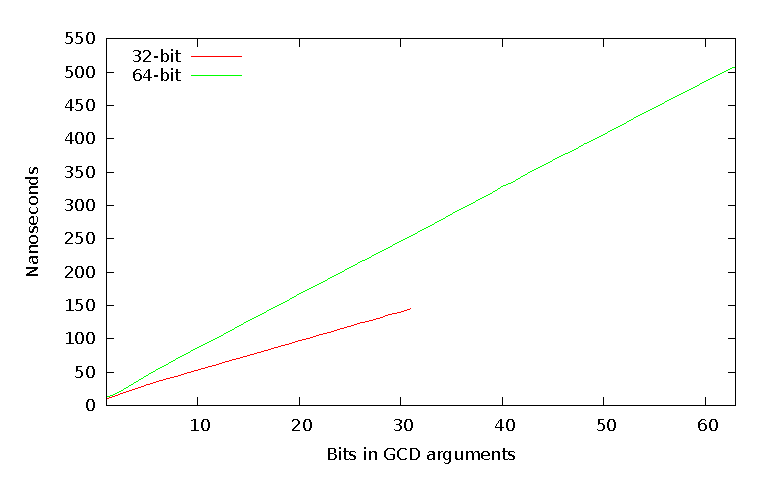
\includegraphics{divrem-32v64}
\caption{Extended Euclidean Algorithm using division with remainder.}
\label{fig:divrem-32v64}
\end{figure}

For Lehmer's GCD, we precomputed a table of 8-bit inputs for the inner GCD computation -- see Figure \ref{fig:lehmer-32v64}. In each case, the 32-bit implementation is faster than the 64-bit implementation.
\begin{figure}[H]
\centering
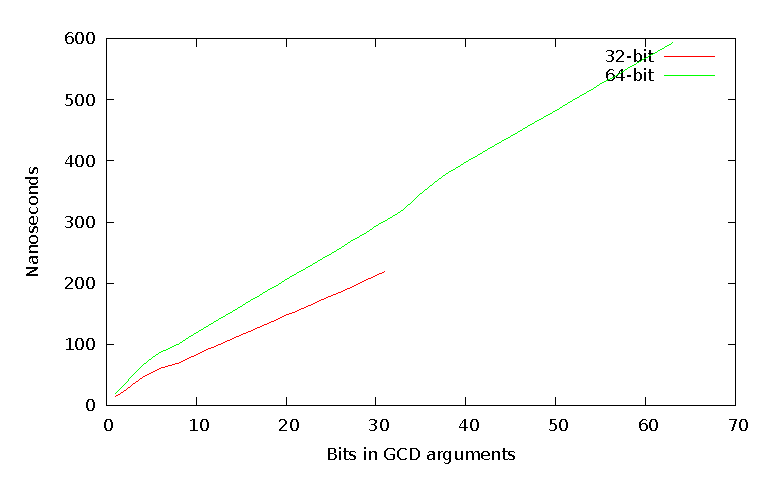
\includegraphics{lehmer-32v64}
\caption{Lehmer's GCD with 8-bit precomputed inner GCD.}
\label{fig:lehmer-32v64}
\end{figure}


The graphs in Figure \ref{fig:stein-32v64} show that for all window sizes from 1 to 5 bits, that the 32-bit version of the right-to-left binary GCD is faster than the 64-bit version.
\begin{figure}[H]
\centering
\mbox{
	\subfigure{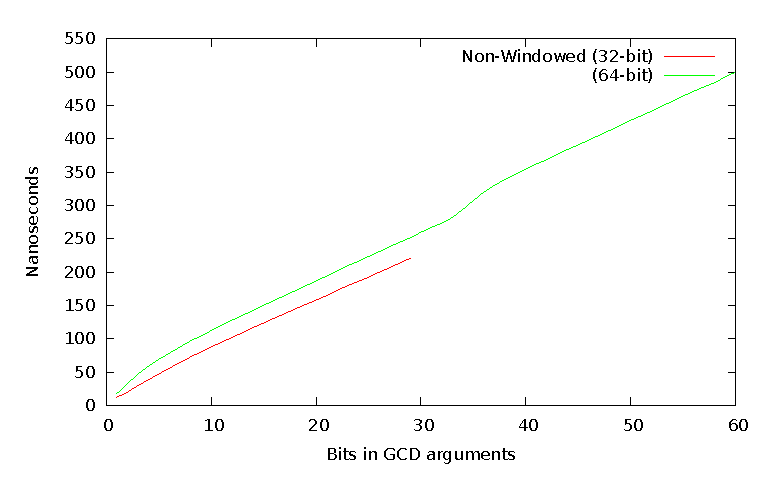
\includegraphics[width=3in]{stein1-32v64}}
	\subfigure{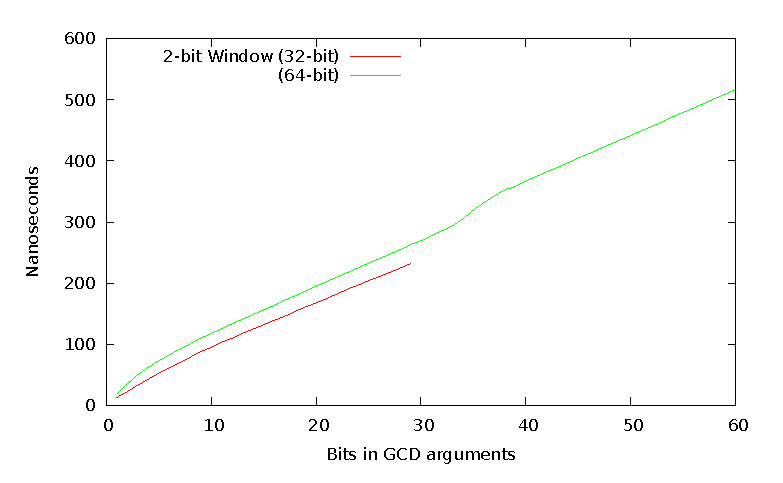
\includegraphics[width=3in]{stein2-32v64}}
}
\mbox{
	\subfigure{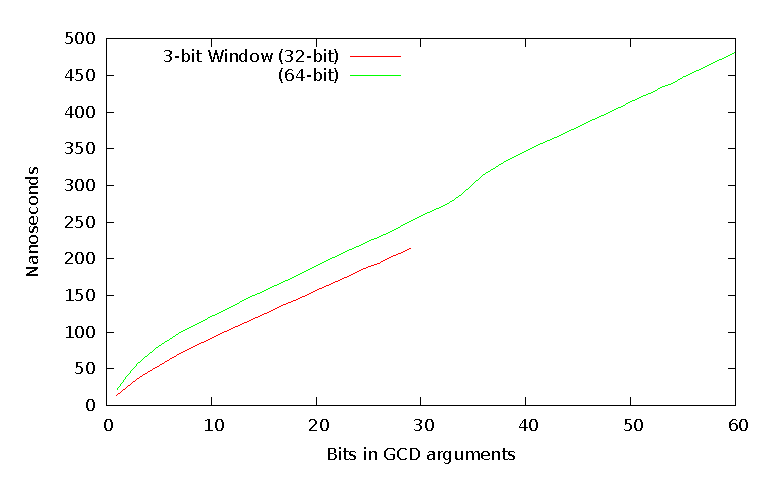
\includegraphics[width=3in]{stein3-32v64}}
	\subfigure{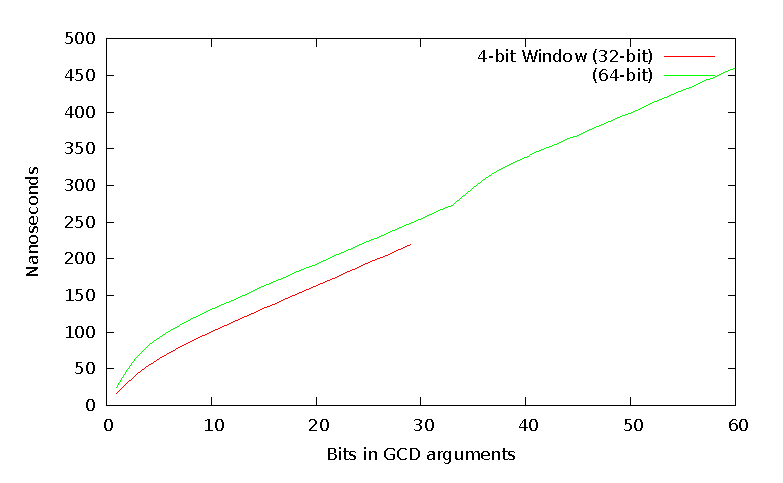
\includegraphics[width=3in]{stein4-32v64}}
}
\mbox{
	\subfigure{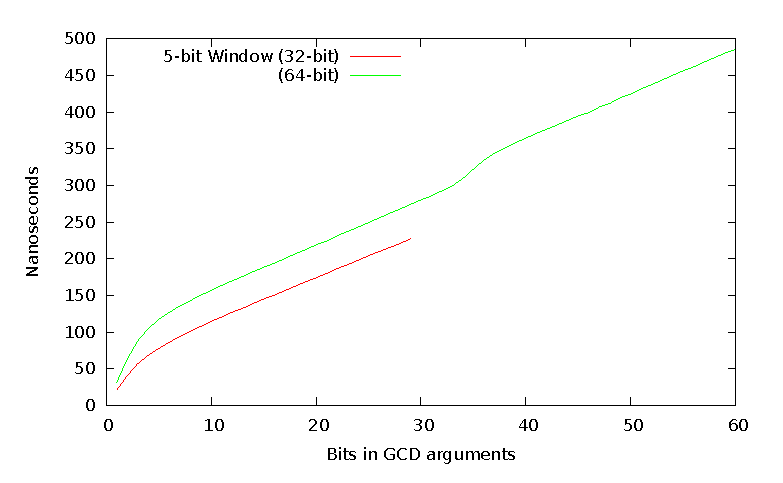
\includegraphics[width=3in]{stein5-32v64}}
}
\caption{Performance of varying the window size of the right-to-left binary GCD.}
\label{fig:stein-32v64}
\end{figure}

The left-to-right variant of the binary GCD proposed by Shallit and Sorenson is shown in figure \ref{fig:shallit-32v64}.  Here the 32-bit implementation is slightly faster than the 64-bit implementation.

\begin{figure}[H]
\centering
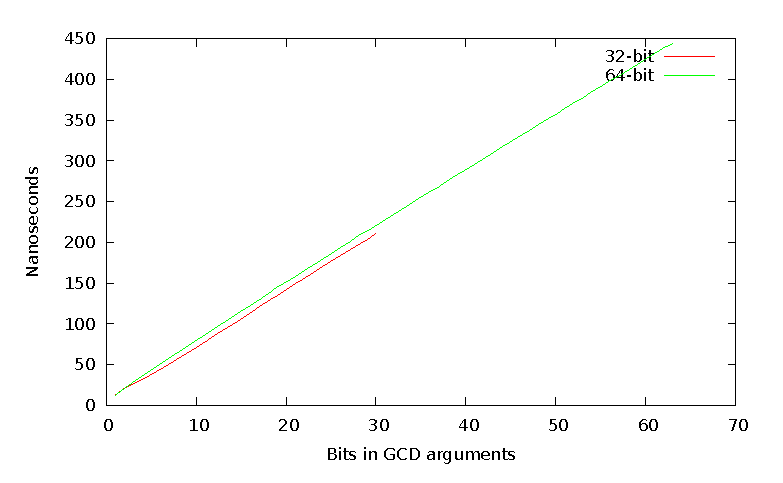
\includegraphics{shallit-32v64}
\caption{Left-to-Right binary GCD of Shallit and Sorenson.}
\label{fig:shallit-32v64}
\end{figure}

Lastly, our simplified version of the left-to-right binary GCD is shown in figure \ref{fig:binary_l2r-32v64}.  In this case, the benefit, if any, to using a 32-bit implementation over a 64-bit implementation is negligible\footnote{Nanosecond differences between the two versions could be attributed to timing inaccuracies.}.

\begin{figure}[H]
\centering
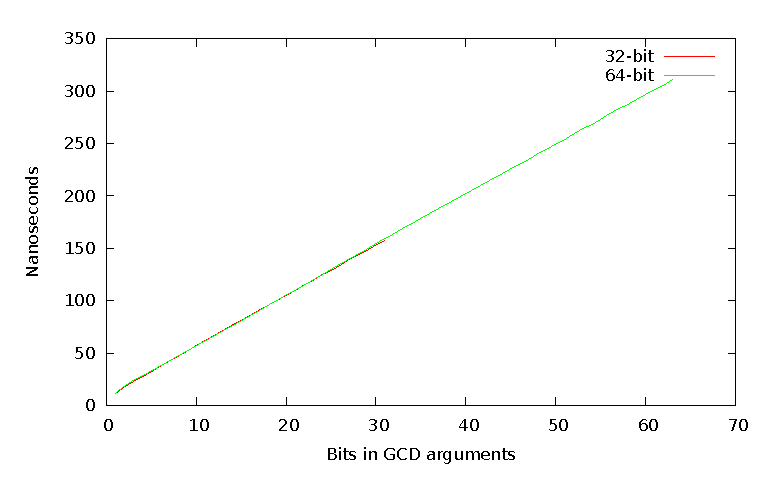
\includegraphics{binary_l2r-32v64}
\caption{Simplified Left-to-Right binary GCD.}
\label{fig:binary_l2r-32v64}
\end{figure}

Note that the 32-bit versions of the right-to-left binary GCD are only accurate up to 29-bits (ignoring sign), while the 64-bit versions are only accurate to 60-bits. All other 32-bit implementations are accurate to 31-bits\footnote{The input is less than or equal to 31-bits, since in a two's complement representation the sign of the input variable takes the most significant bit and accounts for all 32-bits.} and all 64-bit implementations are accurate to 63-bits\footnote{Similar to the 32-bit implementation, the most significant bit represents the sign of the integer.}.

Since the 32-bit implementation of each algorithm is at least no slower than the 64-bit implementation, when comparing the different algorithms, we always prefer the 32-bit implementation of each when the algorithm is known to be accurate for the size of the inputs.

Both the Extended Euclidean Algorithm and Lehmer's GCD use division with remainder to compute their result, so we first compare our implementations of both.  Figure \ref{fig:divrem-vs-lehmer} shows that the Extended Euclidean Algorithm is always faster.

\begin{figure}[H]
\centering
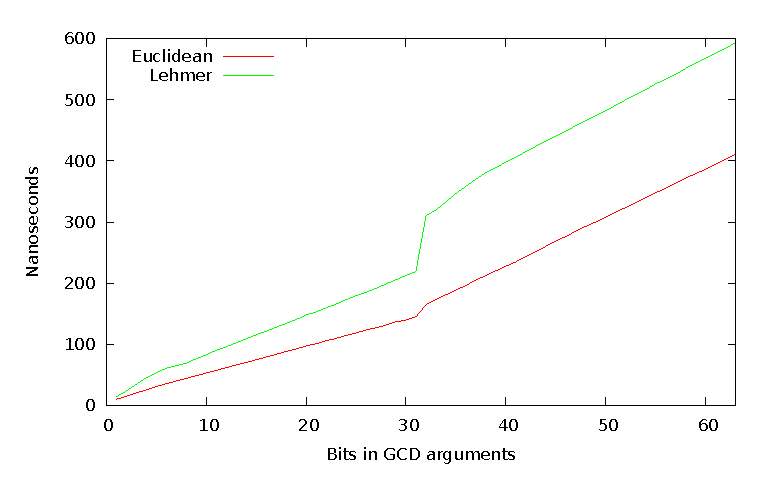
\includegraphics{divrem-vs-lehmer}
\caption{Extended Euclidean Algorithm compared to Lehmer's GCD using precomputed 8-bit words.}
\label{fig:divrem-vs-lehmer}
\end{figure}

In Figure \ref{fig:steins}, we compare each of our windowed implementations of the right-to-left binary GCD.  Larger windows trade off precomputation against the likelihood that a number will be divisible by some power of two. You can see that the non-windowed version is most efficient for inputs less than 16-bits in size, at which point the 3-bit windowed version is best until 30 bits.  After 30 bits, the 4-bit windowed version out performs other window sizes in the range with which we experimented.  In the 64-bit implementation, the slope of the 5-bit windowed version is the lowest and so presumably it would out perform the 4-bit window once inputs were large enough.
\begin{figure}[H]
\centering
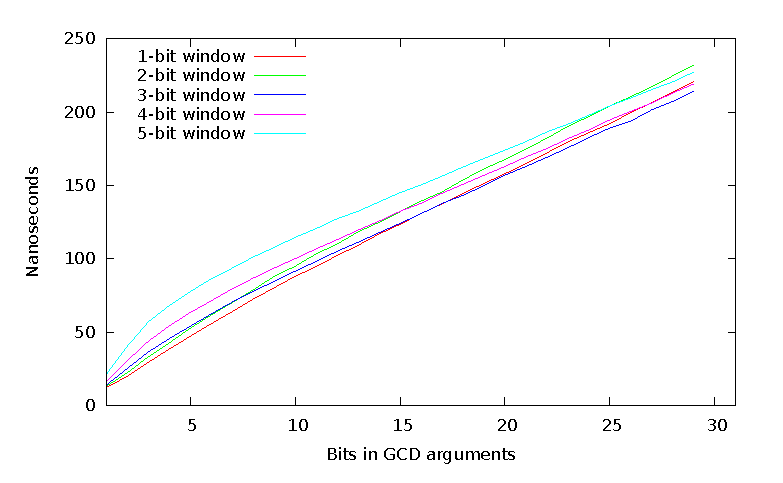
\includegraphics{steins-32}
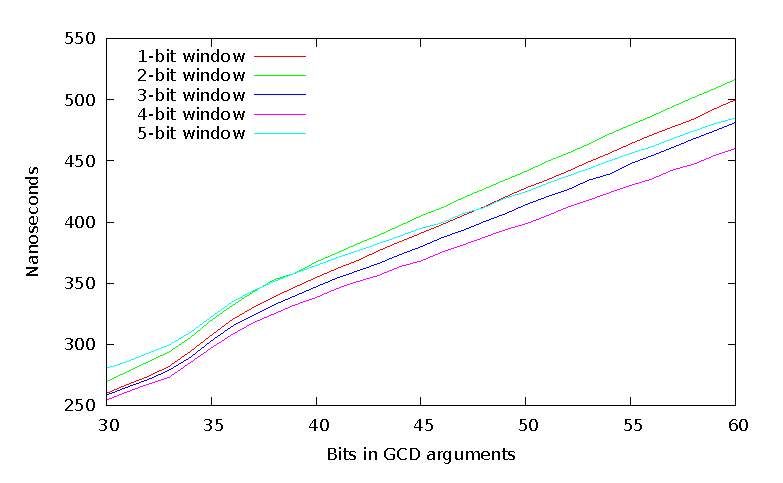
\includegraphics{steins-64}
\caption{Windowed right-to-left binary GCDs.}
\label{fig:steins}
\end{figure}

Figure \ref{fig:shallit-vs-binary_l2r} compares the left-to-right binary GCD proposed by Shallit and Sorenson to our own simplified version.  
\begin{figure}[H]
\centering
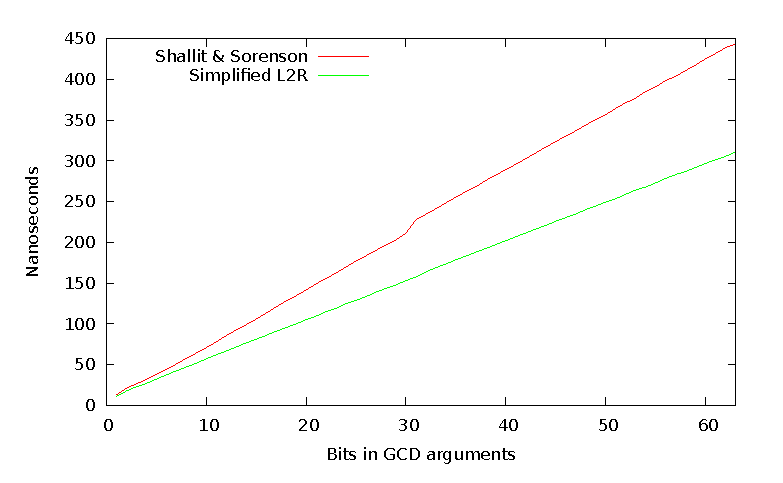
\includegraphics{shallit-vs-binary_l2r}
\caption{Shallit and Sorenson compared to our simplified left-to-right binary GCD.}
\label{fig:shallit-vs-binary_l2r}
\end{figure}

Our implementation of the Euclidean Algorithm always out performs Lehmer's GCD.  For our implementations of the right-to-left binary GCD, among the 32-bit implementations, the non-windowed and the 3-bit windowed versions perform well.  For the 64-bit implementation, the 4-bit windowed version out performs the other window sizes.  Finally, for the left-to-right variants of the binary GCD, our simplified version always out performs the approach proposed by Shallit and Sorenson.  In Figure \ref{fig:all-gcd}, we compare these top performers.  For integer inputs less than 32-bits, the standard Euclidean Algorithm performs best, and for inputs between 32-bits and 64-bits, our simplified left-to-right binary GCD is fastest.
\begin{figure}[H]
\centering
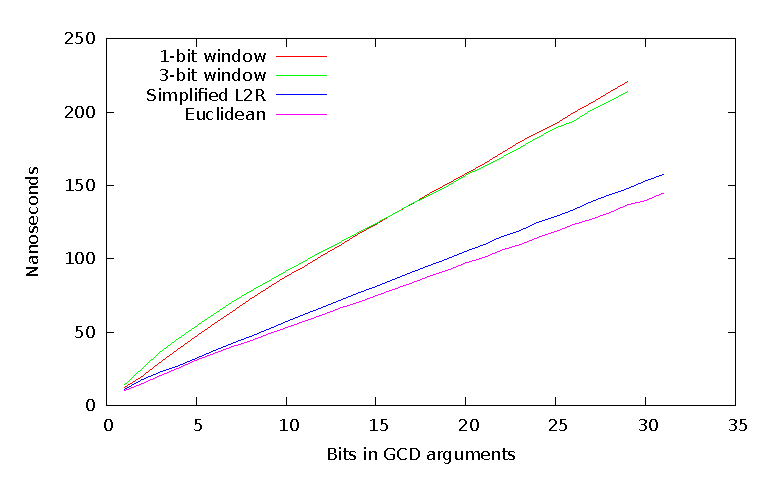
\includegraphics{all-32}
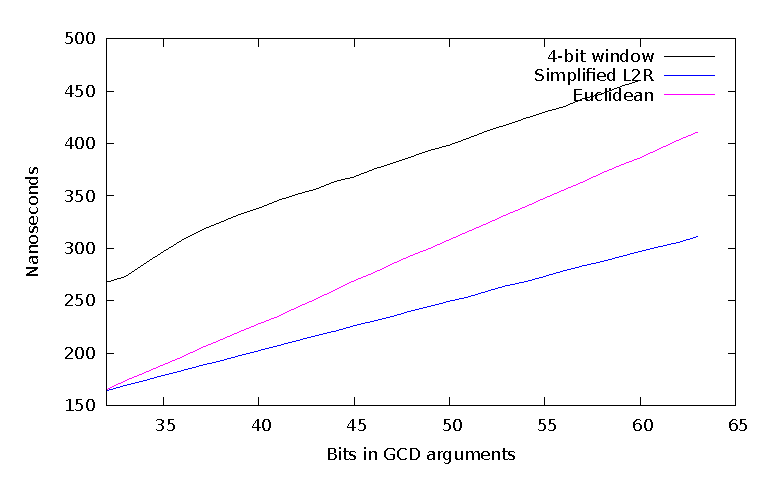
\includegraphics{all-64}
\caption{Euclidean vs windowed right-to-left binary vs Simplified left-to-right binary.}
\label{fig:all-gcd}
\end{figure}

Since the Euclidean Algorithm and our simplified left-to-right binary GCD are our fastest implementations for inputs less than 64-bits, we extended both to work on 128-bit integers.  We also compared these with the implementation of the extended GCD algorithm from the GNU Multiple Precision (GMP) library.  Figure \ref{fig:mpzgcd} show that our implementations out perform the implementation in GMP for inputs smaller than 64-bits.
\begin{figure}[H]
\centering
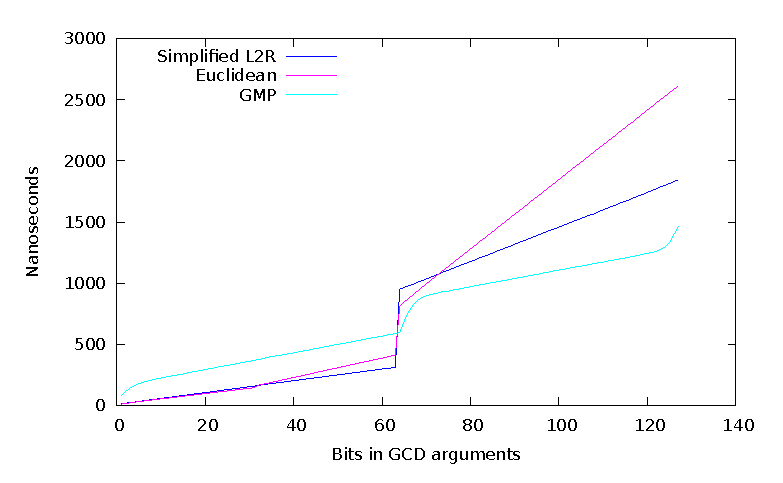
\includegraphics{mpzgcd}
\caption{Euclidean vs our simplified left-to-right binary vs GNU Multiple Precision library.}
\label{fig:mpzgcd}
\end{figure}


\bigbreak
\section{Ideal Arithmetic}
\label{sec:idealArithmetic}

In the previous section, we demonstrated results that lead to practical improvements in computing the extended GCD -- a key operation in reduced ideal multiplication.  In this section, we discuss our implementation of ideal arithmetic.  To improve the performance of ideal arithmetic, we specialized implementations to use at most a single machine word, i.e.\ 64-bits, or at most two machine words, i.e.\ 128-bits.  We also have a reference implementation using GMP that works for unbounded discriminant sizes.  Our 64-bit implementation of ideal arithmetic is accurate for negative discriminants up to 59-bits  in size, while our 128-bit implementation of ideal arithmetic is accurate for discriminants up to 118-bits.

\subsection{Specialized Implementations of Ideal Arithmetic}

Throughout this thesis, we represent an ideal class $[\mathfrak a]$ using the $\ZZ$-module for the reduced ideal representative $\mathfrak a = [a, (b + \sqrt{\Delta})/2]$.  Ideal class multiplication and ideal reduction use the value $c = (b^2 - \Delta)/4a$, which is also useful in determining if an ideal is an ambiguous ideal\footnote{Recall that an ideal is ambiguous if $b=0$, $a=b$, or $a=c$.}.  For this reason, our implementation represents an ideal class using the triple $(a, b, c)$.  Since there are many elements in a given ideal class group, $Cl_\Delta$, we also maintain a representation of the group\footnote{The group representation also includes all intermediate integers needed for use by the GMP library.  The reason for this is that GMP integers are managed on the heap, and preallocating them alongside the representation of the group reduces the overhead of managing them during ideal class group operations.}, which includes the discriminant $\Delta$.

In Subsections \ref{subsec:nucomp}, \ref{subsec:nudupl}, and \ref{subsec:nucube} we introduced algorithms for fast ideal class multiplication, squaring, and cubing.  These compute a termination bound for the partial extended GCD useful for computing the partially reduced coefficients of the product ideal class.  In all cases, the termination bound contains the coefficient $|\Delta/4|^{1/4}$.  Since the coefficients of the partial extended GCD are integers, we instead compute $\ceil{|\Delta/4|^{1/4}}$ as well as $\ceil{|\Delta/4|^{1/2}}$ and tie both to our representation of the class group.  The reason we store $\ceil{|\Delta/4|^{1/2}}$ is that the termination bound for fast ideal multiplication is
\[
\sqrt{a_1/a_2}|\Delta/4|^{1/4} = \sqrt{(a_1/a_2) |\Delta/4|^{1/2}} \approx \sqrt{(a_1/a_2) \ceil{|\Delta/4|^{1/2}}}.
\]
In fast ideal squaring, the bound is simply $|\Delta/4|^{1/4}$ and in fast ideal cubing the bound is $\sqrt{a_1}|\Delta/4|^{1/4} \approx \sqrt{a_1\ceil{|\Delta/4|^{1/2}}}$. By approximating the termination bound, we can speed the arithmetic at the expense of additional reduction steps. We note here that we compute the values $\ceil{|\Delta/4|^{1/2}}$ and $\ceil{|\Delta/4|^{1/4}}$ as accurately as possible, since these are only computed once per class group and then stored with the representation of the group.

We further approximate the computation of integer square roots when computing the termination bound for fast multiplication.  We note that 
\begin{equation*}
\begin{array}{rrlrlr}
	& x^{1/2} &=& 2^{(\log_2x)/2} &\approx& 2^{\floor{\floor{\log_2x+1}/2}} \\
	\Rightarrow & x / x^{1/2} &=& x / 2^{(\log_2x)/2} &\approx& x / 2^{\floor{\floor{\log_2x+1}/2}},
\end{array}
\end{equation*}
where $\floor{\log_2x+1}$ is the number of bits in the binary representation of $x$.  Using this approximation, we compute the integer square root of $x$ as roughly $\floor{x / 2^{\floor{\floor{\log_2x+1}/2}}}$.  This is simply a bit shift right by half the number of bits in $x$.

Other practical considerations are to minimize the size of variables and intermediate values, as smaller operands often lead to faster arithmetic.  Recall that the discriminant $\Delta$ equals $b^2 - 4ac$.  When $4ac=0$ then $b^2$ is as large as possible and so we obtain the bound $b \le \sqrt\Delta$.  Similarly, when $b^2 = 0$ we obtain the bound $a \le \sqrt{\Delta/4}$ (recall that by Definition \ref{defn:reducedIdeal}, a reduced ideal has $a \le c$).  As such, the variables $a$ and $b$ only require half the memory needed to store $\Delta$.

In our 64-bit implementation, $\Delta$ and $c$ take 64-bits of storage, while both $a$ and $b$ require only 32-bits at most.  As such, we take advantage of 32-bit operations when possible, such as our 32-bit implementations of the extended GCD algorithm.  Similarly in our 128-bit implementation, $\Delta$ and $c$ fit within 128-bits of storage, and both $a$ and $b$ fit within one 64-bit machine word.  Again, we use 64-bit arithmetic when possible, and even 32-bit when operands are small.  However, since intermediates may be larger, we sometimes require the full 64-bits or 128-bits of the implementation.

To keep intermediates small, we compute using residue classes.  For example, Equations \ref{eq:idealProductU} states that we can compute $U \pmod {a_1/s}$ and Equation \ref{eq:idealProductB} allows us to compute $b \pmod{2a}$.  When an intermediate is known to be close to zero, we do not perform a complete division with remainder, but only add or subtract the divisor as appropriate (often using the signed mask discussed in Subsection \ref{subsec:gcdImpl}).  Furthermore, rather than computing the positive remainder, we typically compute the remainder that is closest to zero.  The idea here is to minimize the number of bits required by intermediates in order to avoid overflows as much as possible.

In the specific case of ideal reduction (see Algorithm \ref{alg:reduce}), one step is to compute $b'$ such that $-a < b' \le a$ and $b' \equiv b \pmod{2a}$.  To compute $b \bmod{2a}$ we effectively compute $b = q2a + r$ for $q, r \in \ZZ$ where $|r| < 2a$.  We note that $q = \floor{b/(2a)} = \floor{(b/a)/2}$, and instead compute $b = q'a+r'$ for $q', r' \in \ZZ$ where $|r'| < a$.  Now $q'$ is at least twice $q$.  If $q'$ is even, then $b = q'a + r' = (q'/2)2a + r'$ and we let $b' = r'$. Suppose $q'$ is odd and $r'$ is positive.  Then $b = q'a + r' = (q' + 1)a + (r' - a) = ((q' + 1)/2)2a + (r' - a)$.  Since $0 < r' < a$, we have $b' = r' - a$ and $-a < b' \le a$.  The proof is similar when $q$ is odd and $r'$ is negative. This leads us to the following implementation
\begin{align*}
	b' &= \begin{cases}
		r & \textrm{when $q$ is even} \\
		r - a & \textrm{when $q$ is odd and $r > 0$} \\
		r + a & \textrm{otherwise.}
	\end{cases}
\end{align*}

As with our implementations of the extended GCD algorithms, we optimize this to be free of conditionals.  Using two's complement for fixed sized words, we compute 
\begin{align*}
b   &= q'a + r' & \textrm{\{division with remainder\}}\\
q_m &= -(q \band 1) & \textrm{\{$q_m$ has all bits set when $q$ is odd\}} \\
r_m &= \lnot\texttt{sign\_mask}(r) & \textrm{\{$r_m$ has all bits set when $r \ge 0$\}} \\
a'  &= (a \oplus r_m) - r_m & \textrm{\{negate $a$ when $r_m$ is all set\}} \\
r   &= r' + (a' \band q_m) & \textrm{\{move $r$ towards zero when $q$ is odd\}} \\
d   &= r_m \bor 1 & \textrm{1 when $r < 0$ and $-1$ otherwise} \\
q   &= (q' - (d \band q_m))/2 & \textrm{\{adjust $q$ with respect to $r$\}}
\end{align*}
and finally $b' = r$.

Since we represent an ideal class using the triple $(a, b, c)$, it is necessary to compute a new value $c' = (b'^2 - \Delta)/4a$ after a reduction step.  This can be simplified as
\begin{align*}
	c &= (b^2 - \Delta)/4a \\
	  &= ((2aq + r)^2 - \Delta)/4a \\
	  &= (4a^2q^2 + 4aqr + r^2 - \Delta)/4a \\
	  &= (r^2 - \Delta)/4a + aq^2 + qr \\
	  &= c' + q(aq + r) \\
	  &= c' + q(2aq + r - aq) \\
	  &= c' + q(b - aq) \\
	  &= c' + q(b + r)/2.
\end{align*}
As such, we have
\[
c' = c - q(b + r)/2.
\]
Note, the last step above is obtained by rewriting $b = 2aq + r$ as
\begin{align*}
	b - 2aq &= r \\
	2b - 2aq &= b + r \\
	b - aq &= (b+r)/2.
\end{align*}
Since $b - aq \in \ZZ$, the divide by 2 can be performed with an arithmetic bit shift right. (TODO: Is this published anywhere? should I cite something?)

In the previous section, we fine tuned our implementation of the extended GCD computation.  We further refine our use of it here.  Our derivation of ideal multiplication computes
\[
s = \gcd(a_1, a_2, (b_1+b_2)/2) = Ya_1 + Va_2 + W(b_1+b_2)/2
\]
(this is Equation \ref{eq:idealProductS} from Subsection \ref{subsec:idealMultiply}).  In our algorithm for fast ideal multiplication (Algorithm \ref{alg:nucomp}), we break this computation into two parts: the first computes $s' = \gcd(a_1, a_2) = Y'a_1 + V'a_2$ and the second only computes $s = \gcd(s', (b_1 + b_2)/2) = Vs' + W(b_1 + b_2)/2$ when $s' \neq 1$.  We do this since checking for $s \neq 1$ is relatively inexpensive when compared to performing an extended GCD computation.  In addition to this, however, we note that the coefficient $Y'$ is not used in order to derive the product ideal.  As such, computing it is unnecessary and we can simplify our extended GCD computation by dropping the corresponding column from the computation.  This makes it computationally similar to the partial extended GCD, except for the initial and terminating conditions. Lastly, since our simplified left-to-right binary GCD uses only operations representable by unimodular matrices, it can be used to compute the partially reduced coefficients of the product ideal (i.e.\ the partial extended GCD).  This is a performance improvement over the recurrences used for fast ideal multiplication (Subsection \ref{subsec:nucomp}) when the operands are between 32-bits and 64-bits -- since our GCD experiments show that our simplified left-to-right binary GCD performs the best for this range.

A final performance improvement we make is useful for finding prime ideals.  For a given prime $p$, we would like to find an ideal of the form $[p, (b + \sqrt\Delta)/2]$.  We have $b^2 - 4pc = \Delta$, and so we take everything in the residue class modulo $p$ and get $b^2 \equiv \Delta \pmod p$ or $b \equiv \pm\sqrt\Delta \pmod p$.  Computing $b$, then, is a matter of computing a square root modulo a prime, if one exists.  There are efficient algorithms for this (see \cite{Bach1996}), but since we are generally interested in finding some prime ideal, rather than a specific prime ideal, we instead precompute all square roots modulo each prime $p$ for sufficiently many small $p$.  For our purposes, all primes $p < 1000$ was enough.  Finding $b \equiv \pm\sqrt\Delta \pmod p$ is now a table lookup. Having found a value for $b$, we have not necessarily found a prime ideal $[p, (b + \sqrt\Delta)/2]$.  Since $\Delta = b^2 - 4pc$, this implies that $c = (b^2 - \Delta)/4p$ must have an integral solution.  Our implementation maintains the value $c$ for an ideal class, so we compute $c$ and if $c$ is an integer, than we have found a prime ideal.  Otherwise, we try again for some other prime (usually the smallest prime greater than $p$).


\subsection{Average time for operations}

Here, we demonstrate the performance of our implementations of ideal class arithmetic. Let $k$ be the target number of bits in the discriminant $\Delta$.  We iterate $k$ from 16 to 140, and for each $k$ we repeat the following 10,000 times: We compute two prime numbers $p$ and $q$ such that $p$ is $\floor{k/2}$ bits and $q$ is $k-\floor{k/2}$ bits.  We use the negative of their product $\Delta = -pq$ as the discriminant for a class group, unless $\Delta \not\equiv 1 \pmod 4$. In which case, we try again with a different $p$ and $q$.  We then pick a prime form, $[\mathfrak a]$, randomly from among the primes less than 1000.  To time the performance of squaring and cubing, we iterate 1000 times either $[\mathfrak a] \gets [\mathfrak a^2]$ or $[\mathfrak a] \gets [\mathfrak a^3]$ respectively.  Dividing the total cost by 10,000,000 gives the average time to square or cube an ideal.  For multiplication, we initially set $[\mathfrak b] \gets [\mathfrak a]$.  We then iterate 1000 times the sequence of operations $[\mathfrak c] \gets [\mathfrak a\mathfrak b]$, $[\mathfrak a] \gets [\mathfrak b]$, and $[\mathfrak b] \gets [\mathfrak c]$. Figure \ref{fig:idealArithComparison} shows the results of these timings. For all discriminant sizes, our 64-bit implementation out performs our 128-bit implementation, which out performs our GMP implementation.

\begin{figure}[H]
\centering
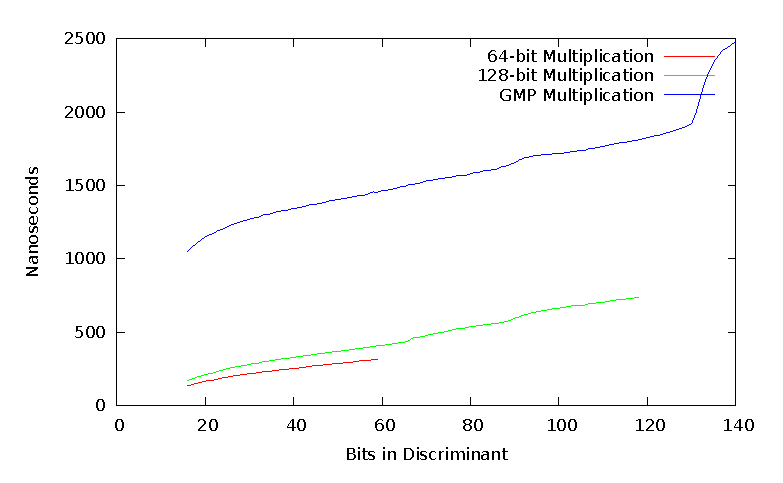
\includegraphics[scale=0.9]{compose-all}
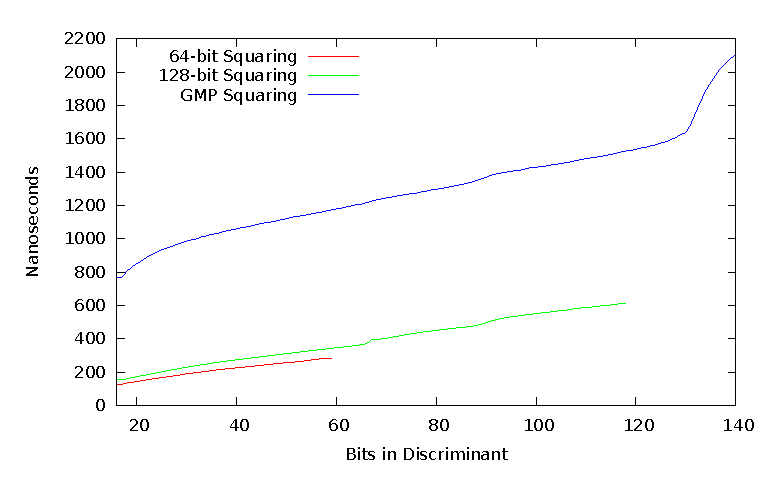
\includegraphics[scale=0.9]{square-all}
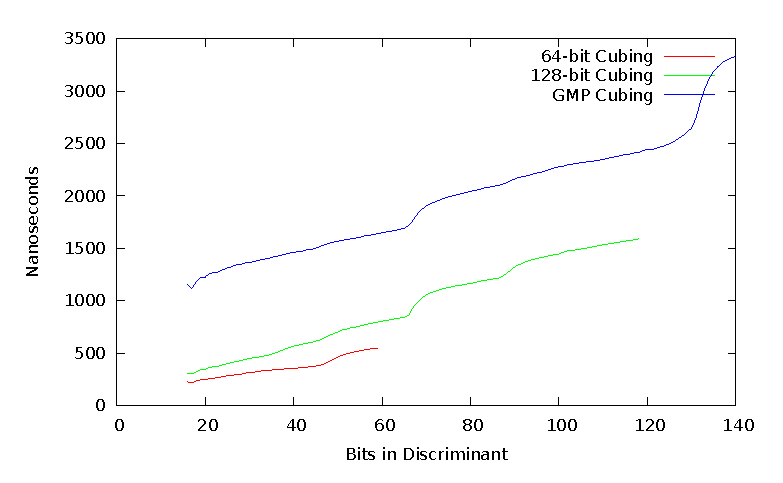
\includegraphics[scale=0.9]{cube-all}
\caption{Average time to multiply, square, or cube ideal classes. The lower the time, the better.}
\label{fig:idealArithComparison}
\end{figure}

Our GMP implementation uses only GMP integers for the ideal class representation, group representation, and intermediate operands.  Intermediate operands during multiplication and squaring always fit within 64-bits for the 64-bit implementation, and 128-bits for the 128-bit implementation.  On the 64-bit implementation, we use 32-bit operations when operands are sufficiently small, and likewise, on the 128-bit implementation, we use 64-bit operations when the operands are sufficiently small.  Intermediate operands during cubing, however, can overflow the target size of the implementation.  In our 64-bit implementation, this is handled by customized assembler (or the use of our 128-bit general arithmetic library).  In our 128-bit implementation, we defer to GMP for overflows.  A result of this is visible in Figure \ref{fig:cubingVsSquareAndMultiply} where we compare the average time to cube an ideal class representative against the average time to multiply a representative with its square.  Our 128-bit implementation of cubing performs more poorly than that of multiplying an ideal with its square.  This is likely because of our reliance on GMP integers for overflow.  Contrast this to our 64-bit implementation that does not use GMP at all, and our GMP implementation that only uses GMP for arithmetic -- in both of these implementations, cubing out performs multiplying an ideal with its square.  For each implementation, we focus the graph on the bit range where that implementation performs the best.

\begin{figure}[H]
\centering
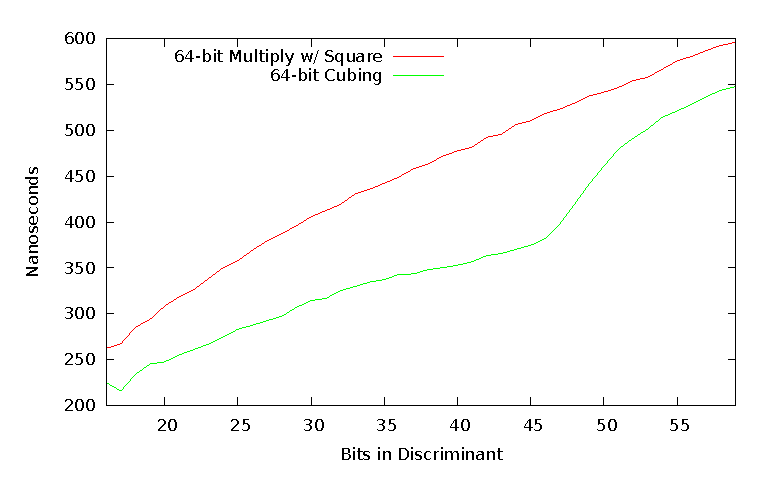
\includegraphics[scale=0.9]{cube-vs-64}
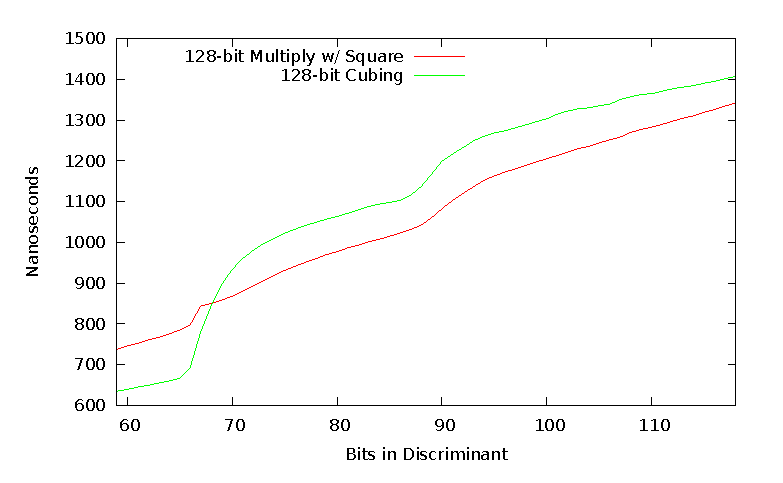
\includegraphics[scale=0.9]{cube-vs-128}
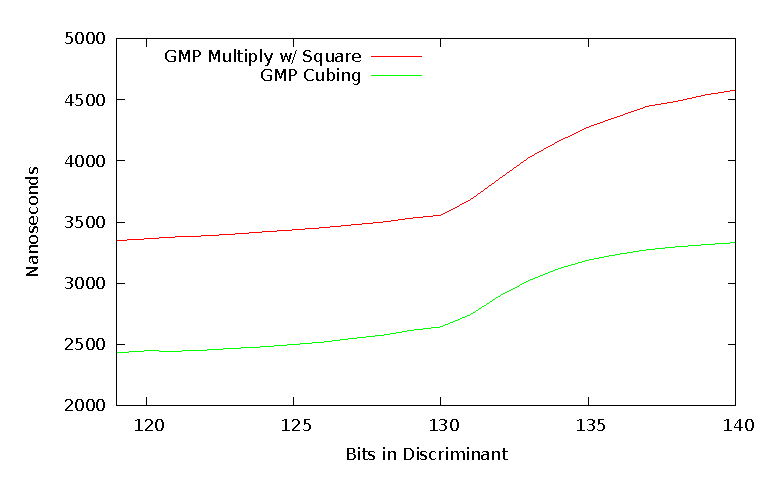
\includegraphics[scale=0.9]{cube-vs-mpz}
\caption{Average time to cube an ideal class compared to the time to square and multiply.  Notice that cubing performs poorly in our 128-bit implementation.}
\label{fig:cubingVsSquareAndMultiply}
\end{figure}

In this section we discussed methods to speed the performance of arithmetic in the ideal class group and we compared the average time of multiplication, squaring, and cubing.  In the next section, we will look at a variety of methods for exponentiating within the ideal class group that we have not discussed previously.  Many of these methods will take the average time of multiplication, squaring, and cubing into account when computing the operations of exponentiation.

\bigbreak
\section{Exponentiation Experiments}
\label{sec:exponentiation}

In this section, we are interested in finding the fastest approach to exponentiating an ideal class representative to a large exponent.  In particular, we consider large exponents that are the product of many small prime powers where the exponent is known in advance.  With the exponent known in advance, this allows us to precompute the sequence of operations in the exponentiation, so that the exponentiation may be as fast as possible without incurring the cost of computing the sequence of operations themselves.

We begin by recalling exponentiation techniques from Chapter \ref{chap:exponentiation}.  These include techniques that use signed and unsigned base two representations, greedy right-to-left and left-to-right double-base representations, and a tree-based approach.  Following this, we consider several greedy variations as well as tree-based extensions of each.  For small exponents (16-bits or less), we consider an incremental search technique, and then extend this to larger exponents by partitioning the exponent into 16-bit blocks. Finally we compare exponentiating by the product of many small primes powers (known as a power primorial) with that of exponentiating by each prime power separately.

TODO: Define \emph{partial representation}.

\subsection{Binary and Right-to-Left Non-Adjacent Form}

In Sections \ref{sec:binaryExp} and \ref{sec:naf} we introduced binary exponentiation and non-adjacent form exponentiation.  Briefly again, binary exponentiation uses the binary representation of an exponent $n$.  The representation can be parsed from high-order to low-order or from low-order to high-order -- we typically refer to this difference as left-to-right or right-to-left respectively.  Using either approach, we use $\floor{\log_2n}$ squares and $\floor{\log_2n}/2$ multiplications on average.

A non-adjacent form exponentiation uses a signed base 2 representation of the exponent such that no two non-zero terms are adjacent\footnote{Non-adjacent form is written as $n=\prod s_i2^i$ for $s_i \in \{0, -1, 1\}$. By ``non-adjacent'' we mean that $s_i \cdot s_{i+1} = 0$ for all $i$.}.  Similarly, when computing a non-adjacent form we can parse the exponent from left-to-right or from right-to-left.  Either direction, we use $\floor{\log_2n} + 1$ squares and $(\floor{\log_2n}+1)/3$ multiplications on average.   

\subsection{Right-to-Left 2,3 Chains}
In Subsection \ref{subsec:rtolChains}, we introduced a method for computing 2,3 chains from low-order to high-order that is a natural extension of the binary representation or non-adjacent form of an exponent.  In this method, we reduce the exponent $n$ by 2 while it is even, and by 3 while it is divisible by 3.  At which point either $n \equiv 1 \pmod 6$ or $n \equiv 5 \pmod 6$ and we add or subtract 1 so that $n$ is a multiple of 6.  The resulting partition of $n$ is then reversed such that the number of squares or cubes in successive terms is monotonically increasing and we can use Algorithm \ref{alg:expWithChain} from Chapter \ref{chap:exponentiation} to compute the exponentiation.

Since this approach evaluates the exponent modulo 3 and may reduce the exponent by 3, efficient methods to compute $n \bmod 3$ and $n/3$ will speed the computation of the chain. Notice that $4 \equiv 1 \pmod 3$.  As such, we can write $n$ as
\[
n = 4 \floor{n/4} + (n \bmod 4) \equiv \floor{n/4} + (n \bmod 4) \pmod 3
\]
and then recursively write $\floor{n/4} \pmod 3$ the same way. This provides us with a method to quickly compute $n \bmod 3$ -- we partition the binary representation of $n$ into \mbox{2-bit} blocks and sum each block modulo 4.  The resulting sum $s$ is $s \equiv n \pmod 3$.  We can further improve the performance of this algorithm when $4$ divides $2^m$ where $m$ is the number of bits in a machine word.  Rather than compute the sum $s \pmod 4$, we compute \mbox{$s \pmod{2^m}$}. After all $m$-bit blocks have been summed, we partition $s$ using words of half the size (assuming 4 divides $2^{m/2}$), sum the half words, and repeat. Since our target architecture (and language) uses 64-bit words, we specialize the algorithm for this case (see Algorithm \ref{alg:fastMod3}).

\begin{algorithm}[h]
\caption{Fast $n \bmod 3$ (adapted from Hacker's Delight \cite{Warren2002}).}
\label{alg:fastMod3}
\begin{algorithmic}[1]
\REQUIRE $n \in \ZZ$.
\ENSURE $n \bmod 3$.
\STATE $s \gets 0$
\FOR {$i$ from $0$ to $\floor{\log_2 n}$ by 64}
	\STATE $t \gets \floor{n / 2^i} \bmod {2^{64}}$
	\STATE $s \gets (s + t) \bmod {2^{64}}$
\ENDFOR
\STATE $s \gets \left(s + \floor{s/{2^{32}}} \right) \bmod {2^{32}}$
\STATE $s \gets \left(s + \floor{s/{2^{16}}} \right) \bmod {2^{16}}$
\STATE $s \gets \left(s + \floor{s/{2^{8}}} \right) \bmod {2^{8}}$
\RETURN $s \bmod 3$ \COMMENT{Lookup from a table with 256 entries.}
\end{algorithmic}
\end{algorithm}

Division by 3 is relatively expensive when compared to computing the remainder.  A common approach is to precompute a single word approximation of the inverse of 3, and then to use multiplication by an approximation of the inverse and then to adjust the result (see \cite{Granlund1994,Warren2002,Moller2011} for additional information).  As the GNU Multiple Precision (GMP) library implements exact division by 3, we use this.


\subsection{Windowed Right-to-Left Chains}

Windowing improves the performance of a right-to-left binary exponentiation and a right-to-left binary GCD computation.  Similarly, we use windowing to improve the performance of a right-to-left 2,3 chain.  Specifically, we experimented with a window size of $2^2 3^2$.  Again, while the exponent is even, we reduce it by 2, and while it is divisible by 3, we reduce it by 3.  In a non-windowed variant, we add or subtract 1 to make the remainder a multiple of 6.  In the windowed variant, we evaluate the exponent $n$ modulo the window $2^2 3^2$, which gives us $n \equiv 1, 5, 7, 11, 13, 17, 19, 23, 25, 29, 31, 35 \pmod {36}$.  As there are 12 different residue classes, and for each residue class we could either add or subtract 1 from $n$, we have $2^{12}$ different strategies to evaluate.  For each strategy, we measured the cost to exponentiate the following 50 different primorials using our implementation of 64-bit and 128-bit ideal class arithmetic (see Section \ref{sec:idealArithmetic}).  For $1 \le k \le 50$, let $j=100k$ and the primorial $P_j=\prod_{i=1}^j p_i$ where $p_i$ is the $i^{\textrm{th}}$ smallest prime.  For 48 out of 50 of the primorials tested, the same strategy lead to the cheapest cost of exponentiation\footnote{For the primorial $P_{200}$, this strategy was the third most efficient, and for $P_{500}$ it was the second most efficient.}, which was to subtract 1 from $n$ when $n \equiv 1, 5, 13, 17, 25, 29 \pmod{36}$ and to add 1 otherwise.

Since the windowed variant of a 2,3 chain computes $n \bmod 36$, we give a fast method for this.  First write $n = 4x + r_4$ for integers $x$ and $r_4$ such that $0 \le r_4 < 4$.  Then write $x = 9y + r_9$ for integers $y$ and $r_9$ such that $0 \le r_9 < 9$.  Substituting the second equation into the first we have
\begin{align*}
	n &= 4(9y + r_9) + r_4 \\
	  &= 36y + 4r_9 + r_4.
\end{align*}
Notice that $(4r_9 + r_4)$ is $n \bmod {36}$ where $r_4 = n \bmod 4$ and $r_9 = \floor{n/4} \bmod 9$. To compute $n \bmod 9$, we point out that $64 \equiv 1 \pmod 9$.  Similar to the case of computing $n \bmod 3$, we write
\[
	n = 64 \floor{n/64} + (n \bmod 64) \equiv \floor{n/64} + (n \bmod 64) \pmod 9
\]
and recursively write $\floor{n/64} \pmod 9$.  To compute $n \bmod 9$, we partition $n$ into blocks of 6-bits (since $2^6 = 64$) and sum each 6-bit block modulo 64.  We then compute the sum $s \bmod 9$.  Again, since our target architecture has 64-bit machine words, we improve upon this by first partitioning $n$ into 192-bit blocks\footnote{We use 192-bit blocks since a 64-bit machine word evenly partitions a 192-bit block and $2^{192} \equiv 1 \pmod 9$.} and compute an intermediate sum of each 192-bit block.  We then partition the intermediate sum into 6-bit blocks and compute the final solution.



\subsection{Left-to-Right 2,3 Representations and Chains}
\label{subsec:ltorChains2}

In Subsection \ref{subsec:ltorChains} we introduced a greedy algorithm for computing 2,3 representations from high-order to low-order.  Briefly, for a given exponent $n$ and for $a_i, b_i \in \ZZgez$ and \mbox{$s_i \in \{-1, 1\}$}, we compute the term $s_i2^{a_i}3^{b_i}$ such that $\left|n-s_i2^{a_i}3^{b_i}\right|$ is as small as possible.  We then recurse on the result $n - s_i2^{a_i}3^{b_i}$.  A chain can be generated by restricting each $a_i$ and $b_i$ such that it is no greater than the $a_{i-1}$ and $b_{i-1}$ from the previous term.  We then reverse the order of terms so that the number of squares and cubes is monotonically increasing. Placing a bound on the number of squares and cubes can also be done globally, i.e.\ for every $a_i, b_i$ we have $0 \le a_i \le A$ and $0 \le b_i \le B$. When a bound is applied globally, the cost of a left-to-right chain or representation varies as the global bound varies.

Figure \ref{fig:dbnsL2rVaryBounds} shows the cost to exponentiate using a left-to-right representation for an exponent that is the product of the first 1000 primes (a number with 11271 bits).  The horizontal axis indicates a global bound $A$ such that all $a_i \le A$.  A global bound $B$ is chosen for the exponent $n$ such that $B = \ceil{\log_3(n/2^A)}$.  The end points of the graph correspond to a representation that uses only cubing and multiplication (on the left side) and a representation that uses only squaring and multiplication (on the right side).  The slope of the graph varies with the ratio of the cost to square relative to the cost to cube.

\begin{figure}[H]
\centering
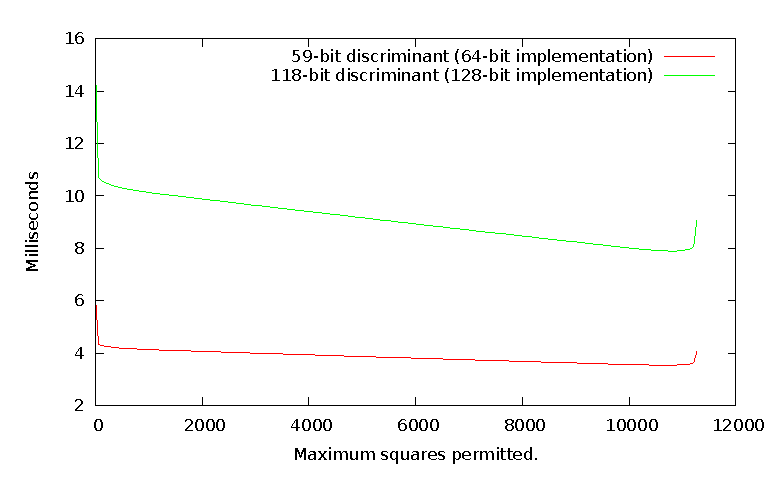
\includegraphics{dbns_l2r_vary_bounds}
\caption{The cost to exponentiate the $1000^{\textrm{th}}$ primorial, $n$, while varying the maximum number of squares permitted, $A$. The maximum number of cubes is $B = \ceil{\log_3(n/2^A)}$.}
\label{fig:dbnsL2rVaryBounds}
\end{figure}

In general, bounding the maximum number of squares and cubes give representations that lead to faster exponentiation in the ideal class group than representations where the number of squares or cubes is left unbound.  For this particular exponent, a representation generated without a global bound takes approximately 7.3 milliseconds for a 59-bit discriminant and 17.2 milliseconds for a 118-bit discriminant.  This is slower than all bounded representations for both implementations.

When the exponent $n$ is known in advance, we generate the 2,3 chain or representation ahead of time and do not include the time to compute the chain or representation in the overall time of the exponentiation.  Since varying the bounds on the number of squares and cubes also varies the cost of exponentiating, in practice we iterate over a range of bounds for the number of cubes in order to find the most efficient chain or representation.  We iterate the bound on the number of cubes rather than squares since $0 \le B \le \ceil{\log_3 n}$ while $0 \le A \le \ceil{\log_2 n}$.

\subsection{Greedy Pruned Trees}

A right-to-left 2,3 chain can be generated by repeatedly reducing the exponent by 2 and 3 and then either adding or subtracting 1 and repeating this process until the exponent is 1.  In the windowed variant, after reducing the exponent by 2 and 3, we had 12 residues modulo $2^2 3^2$ and this lead to $2^{12}$ different strategies for adding or subtracting 1 from the residue.

In Subsection \ref{subsec:pm1Tree}, we discussed a tree based method where a set of at most $k$ of the smallest intermediate exponents are maintained.  At each iteration, each element $x$ in the set generates two new elements $x-1$ and $x+1$.  Again, after reducing each element by powers of 2 and 3, only the $k$ smallest are kept.  That is to say that an element $x$ generates new integral elements $(x \pm 1)/(2^c3^d)$.  As an example, when keeping only the smallest intermediate value, the $10^{\textrm{th}}$ primorial $P_{10} = 6469693230$ generates this representation
\begin{align*}
6469693230 &= 2^1 3^1 (2^1 3^4 (2^6 3^1 (2^2 3^4 (2^2 3^3 - 1) - 1) - 1) - 1) \\
           &= 2^1 3^1 (2^1 3^4 (2^6 3^1 (2^4 3^7 - 2^2 3^4 - 1) - 1) - 1) \\
           &= 2^1 3^1 (2^1 3^4 (2^{10} 3^8 - 2^8 3^5 - 2^6 3^1 - 1) - 1) \\
           &= 2^1 3^1 (2^{11} 3^{12} - 2^9 3^9 - 2^7 3^5 - 2^1 3^4 - 1) \\
           &= 2^{12} 3^{13} - 2^{10} 3^{10} - 2^8 3^6 - 2^2 3^5 - 2^1 3^1.
\end{align*}

Here we consider two variations to the approach of maintaining the $k$ best partial representations.  By ``best'' we mean that we keep the $k$ smallest intermediate values, but that when two values are equal, we compute the cost of the partial chain (with respect to the average cost of multiplication, squaring, and cubing) and say that the value with the smaller cost is better.  The first variation we consider is to generate many new nodes with integer values of the form $(x \pm 2^a3^b)/(2^c3^d)$ for bounded $a$ and $b$ such that $0 \le a \le A$ and $0 \le b \le B$.  Here we chose $A = 2 \ceil{\log_2 n}$ and $B = 3 \ceil{\log_3 n}$ for the input exponent $n$.  The second variation we consider is to include another term before each reduction step, i.e.\ each node generates values of the form $(x \pm 2^{a_1}3^{b_1} \pm 2^{a_2}3^{b_2}) / (2^c 3^d)$.  Notice that the first variation includes the forms $(x \pm 1)/(2^c 3^d)$.  The assumption is that by adjusting $x$ by a fixed length 2,3 representation, we are more likely to find a multiple of a large $2^c3^d$ window than we are by only adding or subtracting one to $x$.

Using the first variant, where we only consider keeping the single best intermediate value, we obtain the following representation
\begin{align*}
6469693230 &= 2^1 3^1 (2^0 3^7 (2^0 3^5 (2^0 3^5 (2^1 3^1 + 2^0 3^0) + 2^3 3^0) + 2^{14} 3^0) + 2^{27} 3^0) \\
&= 2^1 3^1 (2^0 3^7 (2^0 3^5 (2^1 3^6 + 2^0 3^5 + 2^3 3^0) + 2^{14} 3^0) + 2^{27} 3^0) \\
&= 2^1 3^1 (2^0 3^7 (2^1 3^{11} + 2^0 3^{10} + 2^3 3^5 + 2^{14} 3^0) + 2^{27} 3^0) \\
&= 2^1 3^1 (2^1 3^{18} + 2^0 3^{17} + 2^3 3^{12} + 2^{14} 3^7 + 2^{27} 3^0) \\
&= 2^2 3^{19} + 2^1 3^{18} + 2^4 3^{13} + 2^{15} 3^8 + 2^{28} 3^1
\end{align*}

TODO: Come up with an example where successive approaches perform better (if there is one!)

TODO: Say something about $k=1$ being a simple greedy algorithm.

\subsection{The $k$ Best Approximations}

The approach of maintaining a set of the $k$ best partial representations of an exponent can be adapted to that of the left-to-right 2,3 representation from Subsections \ref{subsec:ltorChains} and \ref{subsec:ltorChains2}.  For a given integer $x$ we say that $2^a3^b$ is a best approximation of $|x|$ when $\left||x| - 2^a3^b \right|$ is minimized.  The algorithm for the left-to-right representation finds a best approximation for $x$ and then repeats on the positive difference. However, instead of only iterating on the best approximation, here each value from the set of partial representations generates new values of the form $\left||x| - 2^a3^b\right|$ (being careful to record the sign of $x$), and we keep the $k$ best partial representations.  In this case, we iterate $b$ from $0 \le b \le \ceil{\log_3 |x|}$ and let $a_1 = \floor{\log_2 (x/3^b)}$ and $a_2 = \ceil{\log_2 (x/3^b)}$ (using $a_2 = a_1 + 1$ is sufficient since either $\ceil{\log_2 (x/3^b)} = \floor{\log_2 (x/3^b)}$ or $\ceil{\log_2 (x/3^b)} = \floor{\log_2 (x/3^b)} + 1$). We then use $\left||x|-2^{2_1}3^b\right|$ and $\left||x|-2^{a_2}3^b\right|$ as candidates for the new set.

\subsection{Additive 2,3 Chains}

When the integer to be represented is not too large, Imbert and Philippe \cite{Imbert2010b} give a method to compute the shortest additive strictly chained 2,3 partitions.  These partitions do not permit subtraction and every term is strictly less than and divides all subsequent terms. These partitions take the form
\[
	n = \sum_{i=0}^k 2^{a_i}3^{b_i}
\]
for $a_i, b_i \in \ZZgez$ where $2^{a_i}3^{b_i}$ divides $2^{a_j}3^{b_j}$ and $a_i < a_j$ and $b_i < b_j$ for all $i < j$.

We discussed this technique previously in Subsection \ref{subsec:shortAddChains}.  For our purposes, we modified this algorithm to compute additive 2,3 chains that minimize the average cost of arithmetic in the ideal class group -- the resulting additive 2,3 chains give a better average time for exponentiation, while they may not necessarily be the shortest possible.  

Let $M$, $S$, and $C$ be the average cost to multiply, square, and cube respectively. Our modified function is as follows
\begin{equation*}
s'(n) = \begin{cases}
	\min\{S + s'(n/2), C + s'(n/3)\} & \textrm{when } n \equiv 0 \pmod 6 \\
	M + s'(n-1) & \textrm{when } n \equiv 1 \pmod 6 \\
	S + s'(n/2) & \textrm{when } n \equiv 2 \pmod 6 \\
	\min\{C + s'(n/3), M + S + s'((n-1)/2)\} & \textrm{when } n \equiv 3 \pmod 6 \\
	\min\{S + s'(n/2), M + C + s'((n-1)/3)\} & \textrm{when } n \equiv 4 \pmod 6 \\
	M + S + s'((n-1)/2) & \textrm{when } n \equiv 5 \pmod 6
\end{cases}
\end{equation*}
where $s'(1) = 0$, $s'(2) = S$, and $s'(3) = C$ are the base cases.

We also experimented with computing 2,3 strictly chained partitions that allow for both positive and negative terms.  The corresponding function we used is
\begin{equation*}
f(n) = \begin{cases}
	\min\{S + f(n/2), C + f(n/3)\} & \textrm{when } n \equiv 0 \pmod 6 \\
	\min\{M + f(n-1), M + S + f((n+1)/2)\} & \textrm{when } n \equiv 1 \pmod 6 \\
	\min\{S + f(n/2), M + C + f((n+1)/3)\} & \textrm{when } n \equiv 2 \pmod 6 \\
	\begin{split}\min\{C + f(n/3), M + S + f((n-1)/2),\\M + S + f((n+1)/2)\}\end{split} & \textrm{when } n \equiv 3 \pmod 6 \\
	\min\{S + f(n/2), M + C + f((n-1)/3)\} & \textrm{when } n \equiv 4 \pmod 6 \\
	\min\{M + f(n+1), M + S + f((n-1)/2)\} & \textrm{when } n \equiv 5 \pmod 6 \\
\end{cases}
\end{equation*}
again, where $f(1) = 0$, $f(2) = S$, and $f(3) = C$ are the base cases.  One thing to notice is that the function $s'$ computes a subset of the representations computed by the function $f$, as evidenced by the definitions of these two functions.  Therefore, we expect the average cost to exponentiate using a representation computed by $f$ to be no worse than the average cost to exponentiate using a representation computed by $s$.

Since both functions require an exponential amount of computation in the length of the input, we were only able to compute chains for small exponents.  This is still useful, however, when we consider methods that partition large exponents into smaller blocks using their binary representation, or when we consider multiple exponentiations by a list of prime powers, rather than a single exponentiation by the product of many primes.

In Figure \ref{fig:memoChains} we show the average time to exponentiate ideals with 59-bit and 118-bit discriminants for exponents 1 through 65536.  The graph shows every $512^{\textrm{th}}$ point where the two approaches give different timings\footnote{In the case of the 59-bit discriminant, the timings were the same for 21,816 exponents, and for the 118-bit discriminant, the timings were the same for 16,481 exponents.}.  For every exponent tested, $\pm 2, 3$ chains were on average as fast or faster than additive only chains.
\begin{figure}[H]
\centering
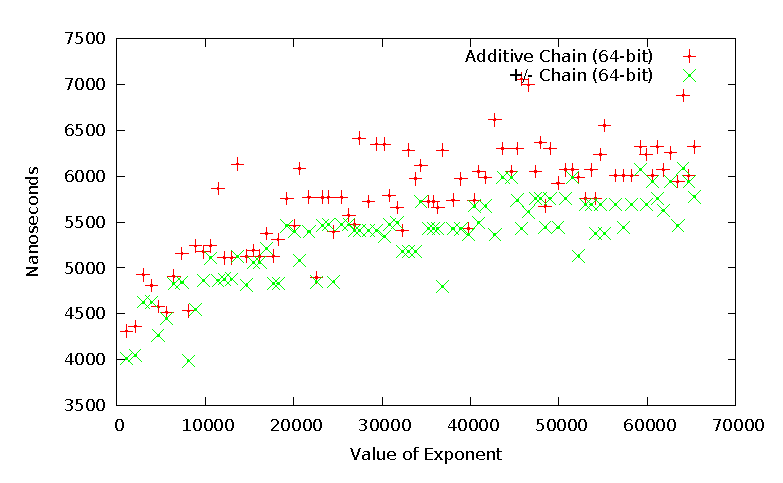
\includegraphics{memo_chains-64}
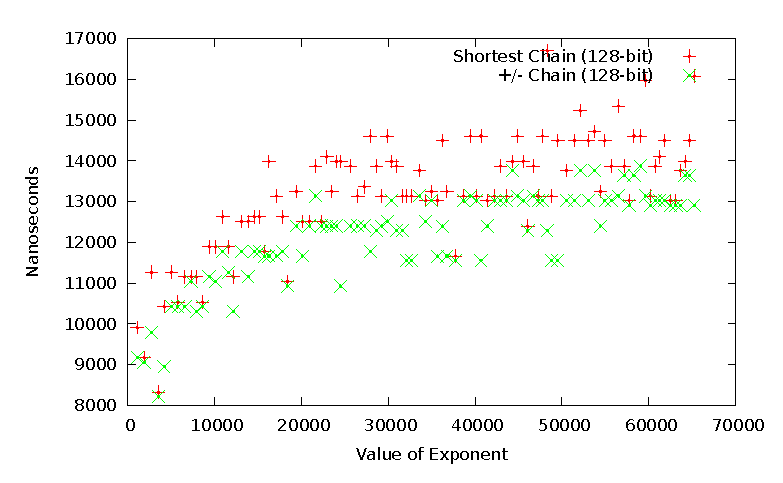
\includegraphics{memo_chains-128}
\caption{Time to exponentiate 16-bit integers using precomputed cost based additive chains and $\pm 1$ chains.}
\label{fig:memoChains}
\end{figure}


\subsection{Searching For 2,3 Representations}

When computing the shortest additive 2,3 chains, Imbert and Phillipe constrained the search space sufficiently in order to exhaustively compute all additive 2,3 strictly chained partitions for the input integer. Here we consider a different approach to searching for representations.  Rather than searching for a representation for a specific integer, we instead iterate over a set of possible representations and compute the integer that is represented.  For each integer represented in the set, we record the cheapest representation encountered.

For example, we first iterated over all single term representations $2^{a_1}3^{b_1}$ for $0 \le a_1 \le A$ and $0 \le b_1 \le B$, and then all two term representations $2^{a_1}3^{b_1} \pm 2^{a_2}3^{b_2}$ for $0 \le a_1 < a_2 \le A$ and $0 \le b_1 < b_2 \le B$.  In general, we computed the set of representations
\[
R = \left\{\sum_{i=1}^k\pm 2^{a_i}3^{b_i} ~:~ 0 \le a_1 < \cdots < a_k \le A \textrm{ and } 0 \le b_1 < \cdots < b_k \le B \right\}
\]
and recorded the lowest average cost of a representation for each integer discovered.

Since this approach to searching for 2, 3 representations is 

\begin{itemize}
\item Algorithm, incorporates cost of multiply, square, cube, cache efficiency
\item 16-bit blocking of exponent
\item Comparison of precomputed representations with greedy approaches
\end{itemize}

\subsection{Exponentiation by fixed primorial}

\subsection{Exponentiation by list of prime powers}

\subsection{Exponentiation by general integers}

\subsection{Experimental Results}

%%%%%%%%%%%%%%%%%%%%%%%%%
% CHAPTER 6             %
% SUPERSPAR EXPERIMENTS %
%%%%%%%%%%%%%%%%%%%%%%%%%
\chapter{SuperSPAR Experiments}

\section{Motivation: How fast can we make SuperSPAR}

\bigbreak
\section{Coprime Finding}
\begin{itemize}
\item Wheeling
\item Sieving
\item Delta Tables
\end{itemize}

\bigbreak
\section{Exponentiation}
\subsection{Bounds for primorial (bound for prime vs exponent)}
\subsection{Primorial vs Prime Powers}
i.e. is it faster to use the product and one exponentiation or individual primes and many exponentations
\subsection{Best primorial bound for n-bit integers}

\section{Time spent on search vs powering}

\section{Sequential prime ideals vs random prime ideals}

\section{Ratio of prime ideals to multipliers}

\section{Best multipliers to use}

\section{Chained Hashing vs OPen Address Hashing}

\section{Empirical search for primorial and step count}
\begin{itemize}
\item Linear, grid, 2d quadratic, 1d grid + binary search on step count.
\item (Quadratic samples at 1/3 and 2/3 and throws away the larger third)
\end{itemize}

\section{Comparison with other algorithms}
\begin{itemize}
\item Pari/GP
\item Custom SQUFOF
\item GNU MSieve
\item GNU-ECM
\item YAFU
\item Flint
\item Maple
\end{itemize}

\chapter{Further Research}

Inclusion into supervisor's ANTL library and hopefully Sage or/and Pari/GP.

Try some extremely large (1Gb+) primorials that are written to disk, powering 2,3 r2l chain of them, and then doing a pollard-rho or something with a smaller primorial for the same number of steps.  The idea being to simulate the original SPAR, but with our library and a few dbns tricks.  Then we try factoring some much larger composites.

This might be interesting to try a discrete log record too.

\section{Other types of Ideal Arithmetic}
For example, the ideal ring of algebraic integers of real quadratic fields.

\section{Function Fields}

For example Hyperelliptic Curves

\section{DBNS with other coprime bases}

Could try tree based approaches where we approximate the cost of the complete chain based on the partial chain, rather than using the smallest remaining exponent and the cost to break ties.

\section{Number systems with three, four, or more bases.}

\section{$\textrm{Super}^2\textrm{SPAR}$}

SuperSPAR with other corprime bases or multiple bases.

In our implementation we choose a primorial, $P$, such that baby steps are coprime to $P$ and giant steps are a multiple of $P$.  We can select a product of small primes that need not be consecutive, e.g. $P = 2 \times 3 \times 11 \times 13$ and then use baby steps coprime to this and giant steps that are a multiple of this.

Also consider parallelization of SuperSPAR using multipliers.  And possibly implementing it on a GPU.


%%%%%%%%%%%%%%%%
% BIBLIOGRAPHY %
%%%%%%%%%%%%%%%%
\bibliographystyle{plain}
\bibliography{Bibliography}


\end{document}
